\documentclass[
%a5paper,
paper=5.5in:8.5in
]{scrbook} 

\title{Persuasion}

\usepackage[romanChapters]{bindery}
\usepackage{dropcaps}
\usepackage{illustrations}
\usepackage{epistolary}

\setdropcaps{FloralCapsNouveau.ttf}
\renewfontfamily\chapterfont{Amarante-Regular.ttf}



\hyphenation{Kel-lynch Mus-grove}

\begin{document}
\frontmatter

\includepdf[width=\coverwidth]{perstitle.png}


\renewcommand*{\chapterheadendvskip}{\vspace{0pt}}
\renewcommand*{\chapterheadstartvskip}{\vspace{0pt}} %because all chapters have head artwork, no need for whitespace
  

\pagestyle{plain}
\renewcommand*\raggedchapter{\centering}

\begin{a4}
	\KOMAoptions{headings=openleft}
\end{a4}

\imagetoc{contents}{0.5}
%\renewcommand{\contentsname}{
\includegraphics[width=.5\linewidth]{contents}}

\tableofcontents
%\clearpage
%
%
\pagestyle{headings}
\renewcommand*{\chapterpagestyle}{plain}




\KOMAoptions{headings=openright}


 
\mainmatter
%!TeX root=../pridetop.tex

\headlesschapter{Chapter \thechapter}

\begin{pictures}
\begin{a4}
	\begin{figure}[t!]
		\centering
		\captionlistentry{Headpiece to Chapter \thechapter}
		\begin{tikzpicture}[remember picture, overlay]  
			\node (img) at ($(current page.north)+(0cm,-10.5cm)$) {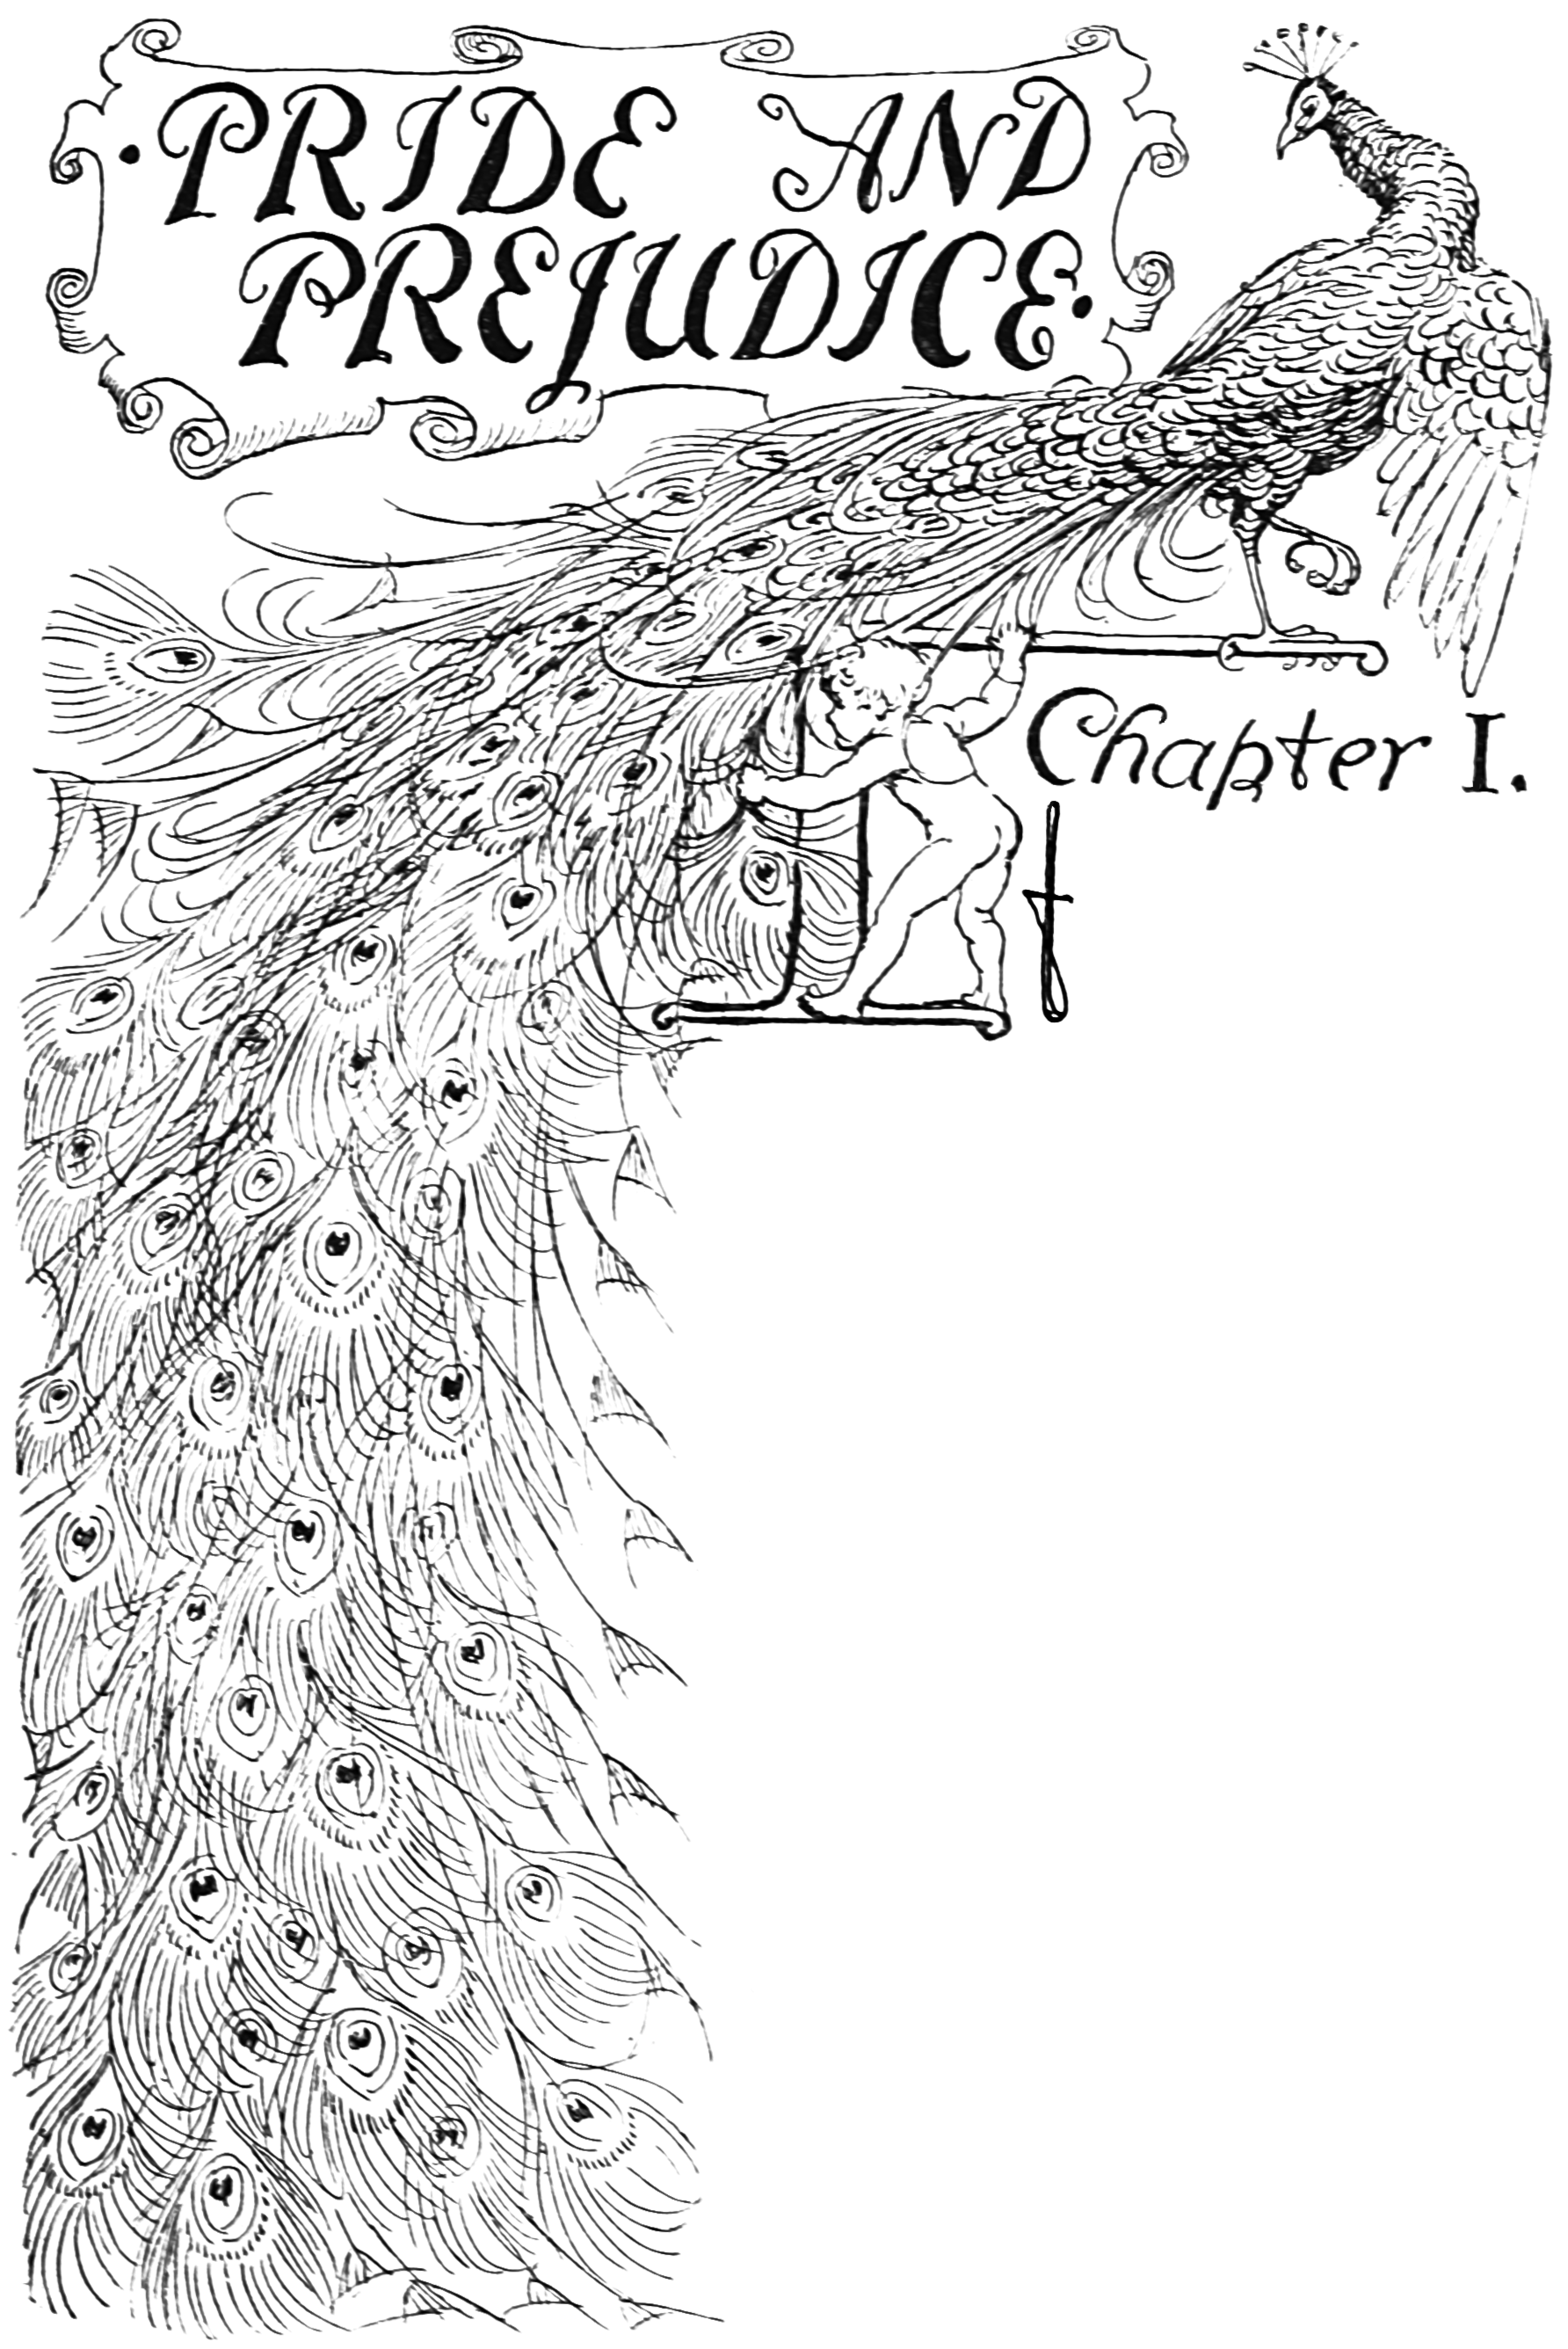
\includegraphics[width=1.15\linewidth]{1top}};
			\node[text width=0.26\textwidth, align=justify] (toptext) at (4.1,1.5) {is a truth universally acknowledged, that};
			\node[below=5.5cm of toptext.east, anchor=east, text width=0.48\textwidth,align=justify] (bottomtext) {
	a single man in possession of a good fortune must be in want of a wife. However little known the feelings or views of such a man may be on his first entering a neighbourhood, this truth is so well fixed in the minds of the surrounding families, that he is considered as the rightful property of some one or other of their daughters.
			\parindent=1em

			<My dear Mr Bennet,> said his lady to him one day, <have you heard that Netherfield Park is let at last?>

			Mr Bennet replied that he had not.

			<But it is,> returned she; <for Mrs Long has just been here, and she told me all about it.>

			Mr Bennet made no answer.

			<Do not you want to know who has taken it?> cried his wife, impatiently.

			<You want to tell me, and I have no objection to hearing it.>
			};
		\end{tikzpicture}
	\end{figure}
\end{a4}

\begin{letter}
	 
	\begin{figure}[t!]
		\centering
		\captionlistentry{Headpiece to Chapter \thechapter}
		\begin{tikzpicture}[remember picture, overlay]
	  
			\node (img) at ($(current page.north)+(0cm,-10.5cm)$) {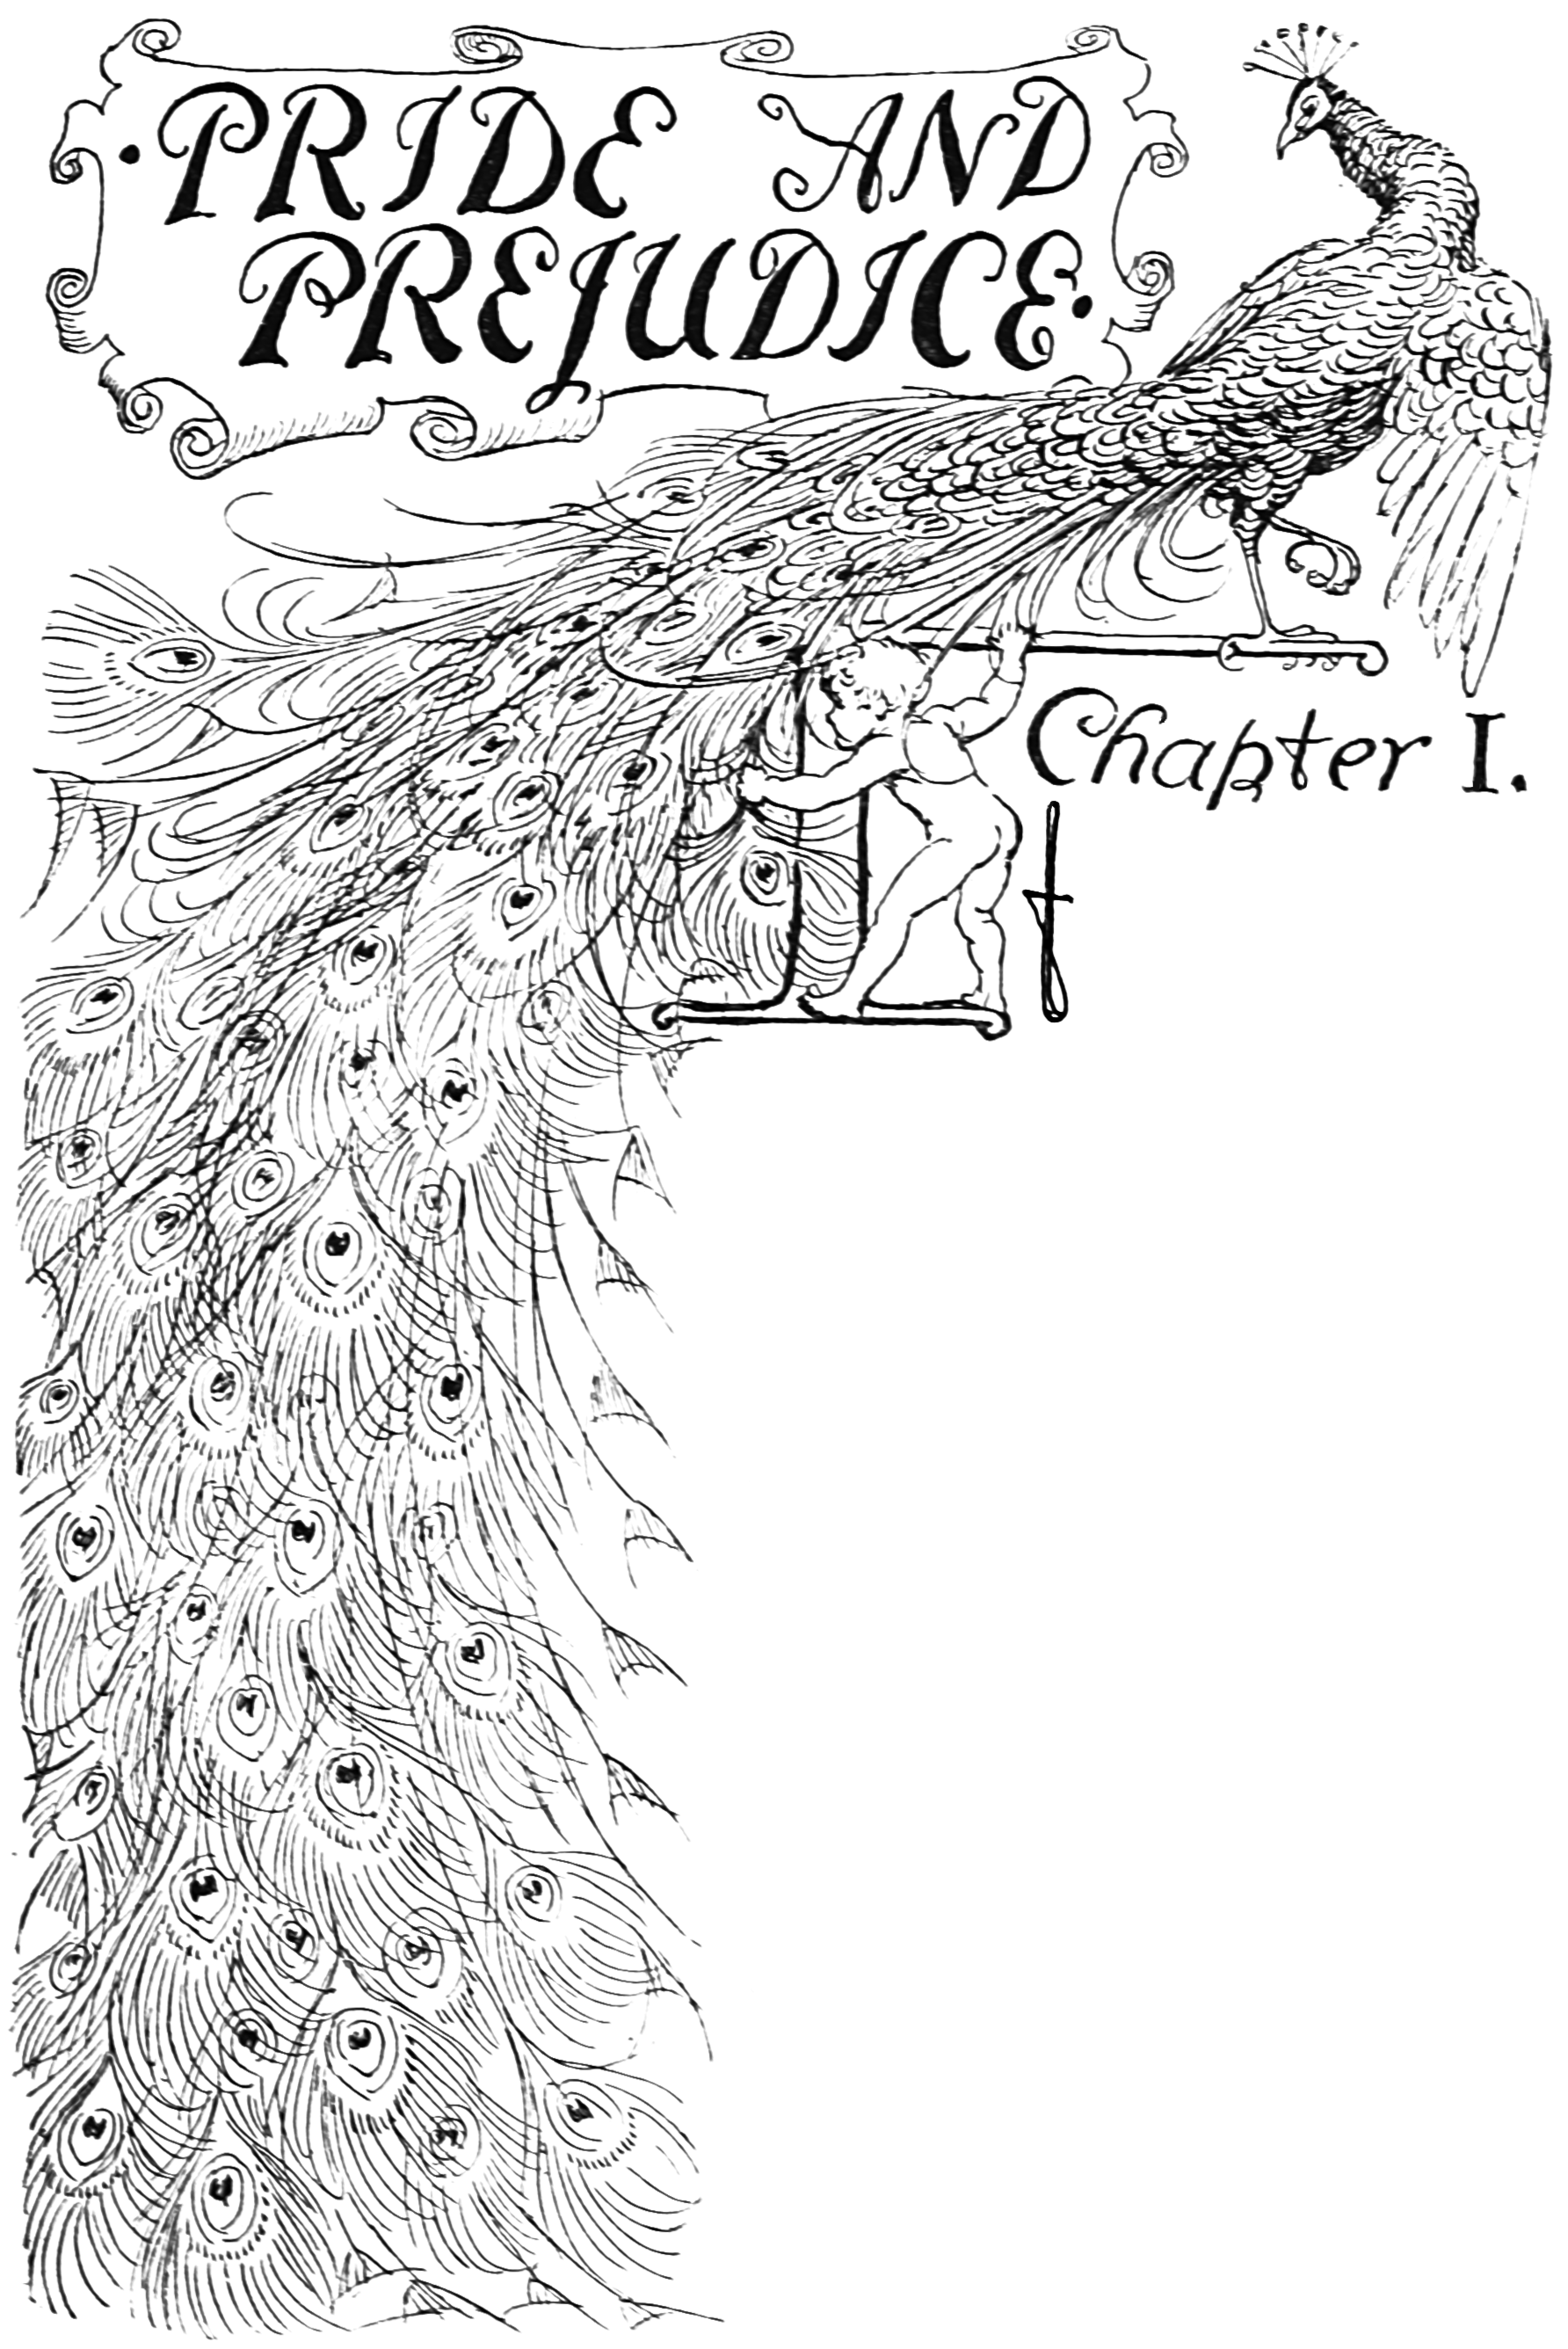
\includegraphics[width=1.2\linewidth]{1top}};
			\node[text width=0.3\textwidth, align=justify] (toptext) at (4.2,1.8) {is a truth universally acknowledged, that a};
			\node[below=5.52cm of toptext.east, anchor=east, text width=0.55\textwidth,align=justify] (bottomtext) {
	single man in possession of a good fortune must be in want of a wife. However little known the feelings or views of such a man may be on his first entering a neighbourhood, this truth is so well fixed in the minds of the surrounding families, that he is considered as the rightful property of some one or other of their daughters.
			\parindent=1em

			<My dear Mr Bennet,> said his lady to him one day, <have you heard that Netherfield Park is let at last?>

			Mr Bennet replied that he had not.

			<But it is,> returned she; <for Mrs Long has just been here, and she told me all about it.>

			Mr Bennet made no answer.

			<Do not you want to know who has taken it?> cried his wife, impatiently.

			<You want to tell me, and I have no objection to hearing it.>
			};
		\end{tikzpicture}
	\end{figure}
%	\enlargethispage{3cm}
\end{letter}

 \thispagestyle{plain}
 \clearpage
\end{pictures}

\begin{placeholder}
It is a truth universally acknowledged, that a single man in possession of a good fortune must be in want of a wife. However little known the feelings or views of such a man may be on his first entering a neighbourhood, this truth is so well fixed in the minds of the surrounding families, that he is considered as the rightful property of some one or other of their daughters.

<My dear Mr Bennet,> said his lady to him one day, <have you heard that Netherfield Park is let at last?>

Mr Bennet replied that he had not.

<But it is,> returned she; <for Mrs Long has just been here, and she told me all about it.>

Mr Bennet made no answer.
<Do not you want to know who has taken it?> cried his wife, impatiently.

<You want to tell me, and I have no objection to hearing it.>
\clearpage
\end{placeholder}

This was invitation enough.

<Why, my dear, you must know, Mrs Long says that Netherfield is taken by a young man of large fortune from the north of England; that he came down on Monday in a chaise and four to see the place, and was so much delighted with it that he agreed with Mr Morris immediately; that he is to take possession before Michaelmas, and some of his servants are to be in the house by the end of next week.>

\begin{figure}[tbh]
\centering

\includegraphics[width=\linewidth]{1camedown}
\captionlistentry{He came down to see the place}
\end{figure}

<What is his name?>

<Bingley.>

<Is he married or single?>

<Oh, single, my dear, to be sure! A single man of large fortune; four or five thousand a year. What a fine thing for our girls!>

<How so? how can it affect them?>

<My dear Mr Bennet,> replied his wife, <how can you be so tiresome? You must know that I am thinking of his marrying one of them.>

<Is that his design in settling here?>

<Design? Nonsense, how can you talk so! But it is very likely that he \textit{may} fall in love with one of them, and therefore you must visit him as soon as he comes.>

<I see no occasion for that. You and the girls may go—or you may send them by themselves, which perhaps will be still better; for as you are as handsome as any of them, Mr Bingley might like you the best of the party.>

<My dear, you flatter me. I certainly \textit{have} had my share of beauty, but I do not pretend to be anything extraordinary now. When a woman has five grown-up daughters, she ought to give over thinking of her own beauty.>

<In such cases, a woman has not often much beauty to think of.>

<But, my dear, you must indeed go and see Mr Bingley when he comes into the neighbourhood.>

<It is more than I engage for, I assure you.>

<But consider your daughters. Only think what an establishment it would be for one of them. Sir William and Lady Lucas are determined to go, merely on that account; for in general, you know, they visit no new comers. Indeed you must go, for it will be impossible for \textit{us} to visit him, if you do not.>

<You are over scrupulous, surely. I dare say Mr Bingley will be very glad to see you; and I will send a few lines by you to assure him of my hearty consent to his marrying whichever he chooses of the girls—though I must throw in a good word for my little Lizzy.>

\begin{figure}[bh!]
\centering
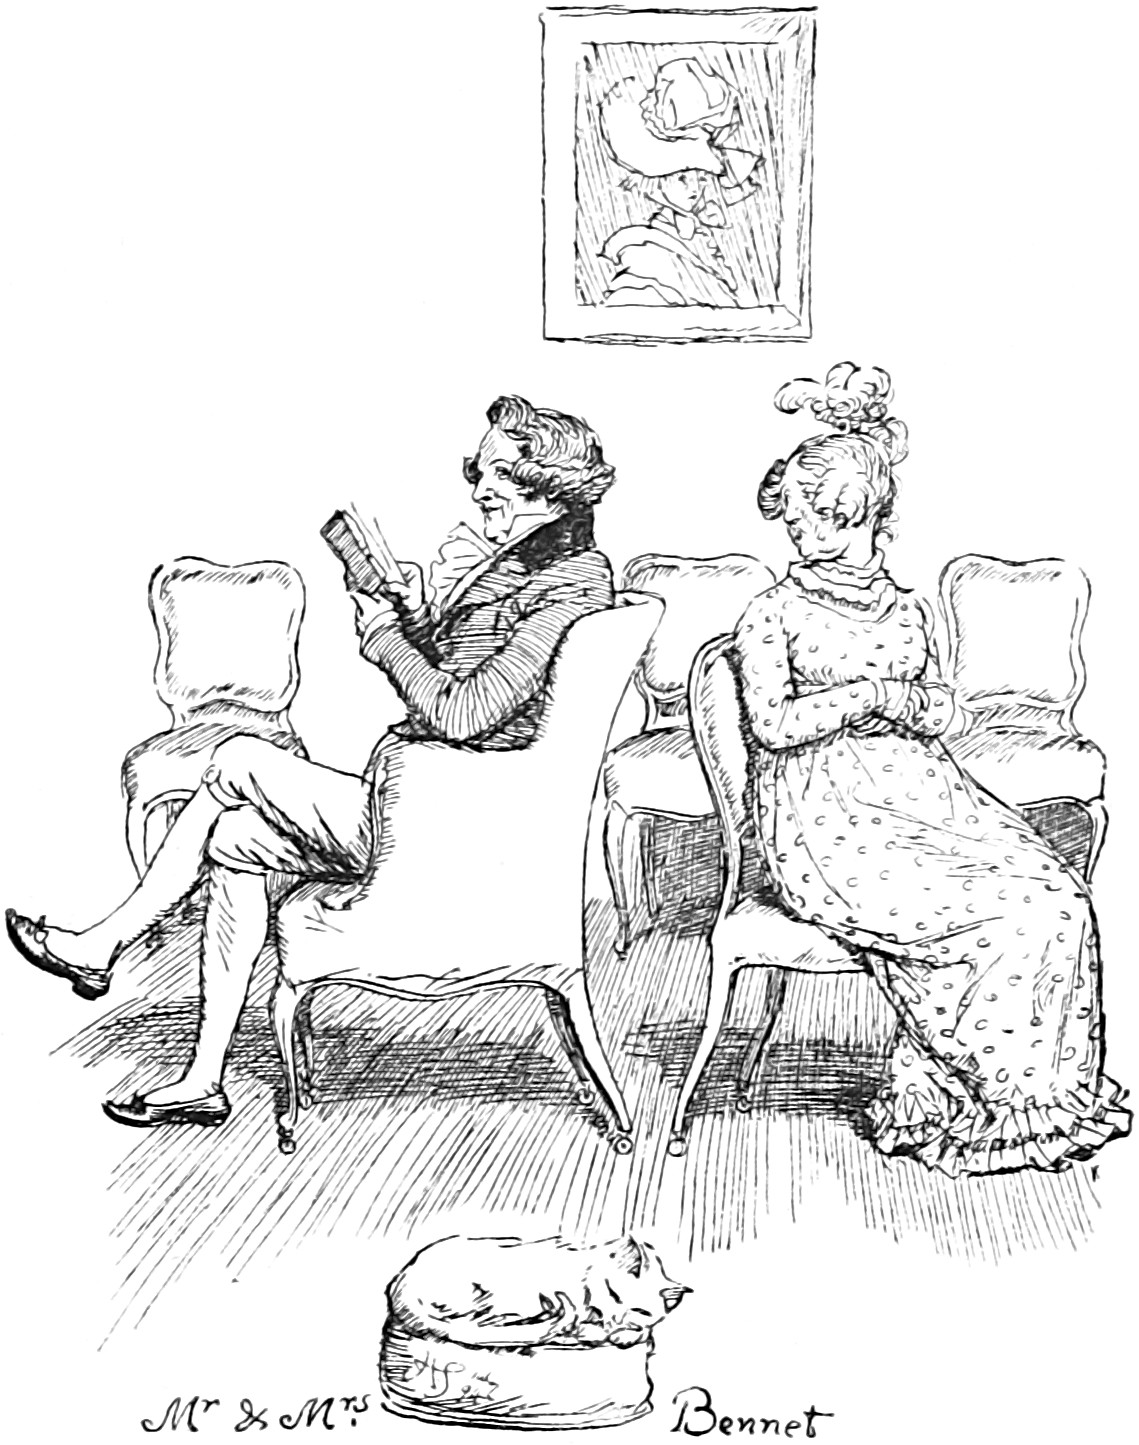
\includegraphics[width=.8\linewidth]{1mrmrs}
\captionlistentry{Mr \& Mrs Bennet}
\end{figure}

<I desire you will do no such thing. Lizzy is not a bit better than the others: and I am sure she is not half so handsome as Jane, nor half so good-humoured as Lydia. But you are always giving \textit{her} the preference.>

<They have none of them much to recommend them,> replied he: <they are all silly and ignorant like other girls; but Lizzy has something more of quickness than her sisters.>

<Mr Bennet, how can you abuse your own children in such a way? You take delight in vexing me. You have no compassion on my poor nerves.>

<You mistake me, my dear. I have a high respect for your nerves. They are my old friends. I have heard you mention them with consideration these twenty years at least.>

<Ah, you do not know what I suffer.>

<But I hope you will get over it, and live to see many young men of four thousand a year come into the neighbourhood.>

<It will be no use to us, if twenty such should come, since you will not visit them.>

<Depend upon it, my dear, that when there are twenty, I will visit them all.>

Mr Bennet was so odd a mixture of quick parts, sarcastic humour, reserve, and caprice, that the experience of three-and-twenty years had been insufficient to make his wife understand his character. \textit{Her} mind was less difficult to develope. She was a woman of mean understanding, little information, and uncertain temper. When she was discontented, she fancied herself nervous. The business of her life was to get her daughters married: its solace was visiting and news.


\chapter[Chapter \thechapter]{} 

 \lettrine[lraise=0.3]{T}{he} little girl performed her long journey in safety; and at Northampton was met by Mrs~Norris, who thus regaled in the credit of being foremost to welcome her, and in the importance of leading her in to the others, and recommending her to their kindness.

Fanny Price was at this time just ten years old, and though there might not be much in her first appearance to captivate, there was, at least, nothing to disgust her relations. She was small of her age, with no glow of complexion, nor any other striking beauty; exceedingly timid and shy, and shrinking from notice; but her air, though awkward, was not vulgar, her voice was sweet, and when she spoke her countenance was pretty. Sir~Thomas and Lady Bertram received her very kindly; and Sir~Thomas, seeing how much she needed encouragement, tried to be all that was conciliating: but he had to work against a most untoward gravity of deportment; and Lady Bertram, without taking half so much trouble, or speaking one word where he spoke ten, by the mere aid of a good-humoured smile, became immediately the less awful character of the two.

The young people were all at home, and sustained their share in the introduction very well, with much good humour, and no embarrassment, at least on the part of the sons, who, at seventeen and sixteen, and tall of their age, had all the grandeur of men in the eyes of their little cousin. The two girls were more at a loss from being younger and in greater awe of their father, who addressed them on the occasion with rather an injudicious particularity. But they were too much used to company and praise to have anything like natural shyness; and their confidence increasing from their cousin's total want of it, they were soon able to take a full survey of her face and her frock in easy indifference.

They were a remarkably fine family, the sons very well-looking, the daughters decidedly handsome, and all of them well-grown and forward of their age, which produced as striking a difference between the cousins in person, as education had given to their address; and no one would have supposed the girls so nearly of an age as they really were. There were in fact but two years between the youngest and Fanny. Julia Bertram was only twelve, and Maria but a year older. The little visitor meanwhile was as unhappy as possible. Afraid of everybody, ashamed of herself, and longing for the home she had left, she knew not how to look up, and could scarcely speak to be heard, or without crying. Mrs~Norris had been talking to her the whole way from Northampton of her wonderful good fortune, and the extraordinary degree of gratitude and good behaviour which it ought to produce, and her consciousness of misery was therefore increased by the idea of its being a wicked thing for her not to be happy. The fatigue, too, of so long a journey, became soon no trifling evil. In vain were the well-meant condescensions of Sir~Thomas, and all the officious prognostications of Mrs~Norris that she would be a good girl; in vain did Lady Bertram smile and make her sit on the sofa with herself and pug, and vain was even the sight of a gooseberry tart towards giving her comfort; she could scarcely swallow two mouthfuls before tears interrupted her, and sleep seeming to be her likeliest friend, she was taken to finish her sorrows in bed.

<This is not a very promising beginning,> said Mrs~Norris, when Fanny had left the room. <After all that I said to her as we came along, I thought she would have behaved better; I told her how much might depend upon her acquitting herself well at first. I wish there may not be a little sulkiness of temper—her poor mother had a good deal; but we must make allowances for such a child—and I do not know that her being sorry to leave her home is really against her, for, with all its faults, it \textit{was}  her home, and she cannot as yet understand how much she has changed for the better; but then there is moderation in all things.>

It required a longer time, however, than Mrs~Norris was inclined to allow, to reconcile Fanny to the novelty of Mansfield Park, and the separation from everybody she had been used to. Her feelings were very acute, and too little understood to be properly attended to. Nobody meant to be unkind, but nobody put themselves out of their way to secure her comfort.

The holiday allowed to the Miss~Bertrams the next day, on purpose to afford leisure for getting acquainted with, and entertaining their young cousin, produced little union. They could not but hold her cheap on finding that she had but two sashes, and had never learned French; and when they perceived her to be little struck with the duet they were so good as to play, they could do no more than make her a generous present of some of their least valued toys, and leave her to herself, while they adjourned to whatever might be the favourite holiday sport of the moment, making artificial flowers or wasting gold paper.

Fanny, whether near or from her cousins, whether in the schoolroom, the drawing-room, or the shrubbery, was equally forlorn, finding something to fear in every person and place. She was disheartened by Lady Bertram's silence, awed by Sir~Thomas's grave looks, and quite overcome by Mrs~Norris's admonitions. Her elder cousins mortified her by reflections on her size, and abashed her by noticing her shyness: Miss~Lee wondered at her ignorance, and the maid-servants sneered at her clothes; and when to these sorrows was added the idea of the brothers and sisters among whom she had always been important as playfellow, instructress, and nurse, the despondence that sunk her little heart was severe.

The grandeur of the house astonished, but could not console her. The rooms were too large for her to move in with ease: whatever she touched she expected to injure, and she crept about in constant terror of something or other; often retreating towards her own chamber to cry; and the little girl who was spoken of in the drawing-room when she left it at night as seeming so desirably sensible of her peculiar good fortune, ended every day's sorrows by sobbing herself to sleep. A week had passed in this way, and no suspicion of it conveyed by her quiet passive manner, when she was found one morning by her cousin Edmund, the youngest of the sons, sitting crying on the attic stairs.

<My dear little cousin,> said he, with all the gentleness of an excellent nature, <what can be the matter?> And sitting down by her, he was at great pains to overcome her shame in being so surprised, and persuade her to speak openly. Was she ill? or was anybody angry with her? or had she quarrelled with Maria and Julia? or was she puzzled about anything in her lesson that he could explain? Did she, in short, want anything he could possibly get her, or do for her? For a long while no answer could be obtained beyond a <no, no—not at all—no, thank you>; but he still persevered; and no sooner had he begun to revert to her own home, than her increased sobs explained to him where the grievance lay. He tried to console her.

<You are sorry to leave Mama, my dear little Fanny,> said he, <which shows you to be a very good girl; but you must remember that you are with relations and friends, who all love you, and wish to make you happy. Let us walk out in the park, and you shall tell me all about your brothers and sisters.>

On pursuing the subject, he found that, dear as all these brothers and sisters generally were, there was one among them who ran more in her thoughts than the rest. It was William whom she talked of most, and wanted most to see. William, the eldest, a year older than herself, her constant companion and friend; her advocate with her mother (of whom he was the darling) in every distress. <William did not like she should come away; he had told her he should miss her very much indeed.> <But William will write to you, I dare say.> <Yes, he had promised he would, but he had told \textit{her}  to write first.> <And when shall you do it?> She hung her head and answered hesitatingly, <she did not know; she had not any paper.>

<If that be all your difficulty, I will furnish you with paper and every other material, and you may write your letter whenever you choose. Would it make you happy to write to William?>

<Yes, very.>

<Then let it be done now. Come with me into the breakfast-room, we shall find everything there, and be sure of having the room to ourselves.>

<But, cousin, will it go to the post?>

<Yes, depend upon me it shall: it shall go with the other letters; and, as your uncle will frank it, it will cost William nothing.>

<My uncle!> repeated Fanny, with a frightened look.

<Yes, when you have written the letter, I will take it to my father to frank.>

Fanny thought it a bold measure, but offered no further resistance; and they went together into the breakfast-room, where Edmund prepared her paper, and ruled her lines with all the goodwill that her brother could himself have felt, and probably with somewhat more exactness. He continued with her the whole time of her writing, to assist her with his penknife or his orthography, as either were wanted; and added to these attentions, which she felt very much, a kindness to her brother which delighted her beyond all the rest. He wrote with his own hand his love to his cousin William, and sent him half a guinea under the seal. Fanny's feelings on the occasion were such as she believed herself incapable of expressing; but her countenance and a few artless words fully conveyed all their gratitude and delight, and her cousin began to find her an interesting object. He talked to her more, and, from all that she said, was convinced of her having an affectionate heart, and a strong desire of doing right; and he could perceive her to be farther entitled to attention by great sensibility of her situation, and great timidity. He had never knowingly given her pain, but he now felt that she required more positive kindness; and with that view endeavoured, in the first place, to lessen her fears of them all, and gave her especially a great deal of good advice as to playing with Maria and Julia, and being as merry as possible.

From this day Fanny grew more comfortable. She felt that she had a friend, and the kindness of her cousin Edmund gave her better spirits with everybody else. The place became less strange, and the people less formidable; and if there were some amongst them whom she could not cease to fear, she began at least to know their ways, and to catch the best manner of conforming to them. The little rusticities and awkwardnesses which had at first made grievous inroads on the tranquillity of all, and not least of herself, necessarily wore away, and she was no longer materially afraid to appear before her uncle, nor did her aunt Norris's voice make her start very much. To her cousins she became occasionally an acceptable companion. Though unworthy, from inferiority of age and strength, to be their constant associate, their pleasures and schemes were sometimes of a nature to make a third very useful, especially when that third was of an obliging, yielding temper; and they could not but own, when their aunt inquired into her faults, or their brother Edmund urged her claims to their kindness, that <Fanny was good-natured enough.>

Edmund was uniformly kind himself; and she had nothing worse to endure on the part of Tom than that sort of merriment which a young man of seventeen will always think fair with a child of ten. He was just entering into life, full of spirits, and with all the liberal dispositions of an eldest son, who feels born only for expense and enjoyment. His kindness to his little cousin was consistent with his situation and rights: he made her some very pretty presents, and laughed at her.

As her appearance and spirits improved, Sir~Thomas and Mrs~Norris thought with greater satisfaction of their benevolent plan; and it was pretty soon decided between them that, though far from clever, she showed a tractable disposition, and seemed likely to give them little trouble. A mean opinion of her abilities was not confined to \textit{them}. Fanny could read, work, and write, but she had been taught nothing more; and as her cousins found her ignorant of many things with which they had been long familiar, they thought her prodigiously stupid, and for the first two or three weeks were continually bringing some fresh report of it into the drawing-room. <Dear mama, only think, my cousin cannot put the map of Europe together—or my cousin cannot tell the principal rivers in Russia—or, she never heard of Asia Minor—or she does not know the difference between water-colours and crayons!—How strange!—Did you ever hear anything so stupid?>

<My dear,> their considerate aunt would reply, <it is very bad, but you must not expect everybody to be as forward and quick at learning as yourself.>

<But, aunt, she is really so very ignorant!—Do you know, we asked her last night which way she would go to get to Ireland; and she said, she should cross to the Isle of Wight. She thinks of nothing but the Isle of Wight, and she calls it \textit{the Island}, as if there were no other island in the world. I am sure I should have been ashamed of myself, if I had not known better long before I was so old as she is. I cannot remember the time when I did not know a great deal that she has not the least notion of yet. How long ago it is, aunt, since we used to repeat the chronological order of the kings of England, with the dates of their accession, and most of the principal events of their reigns!>

<Yes,> added the other; <and of the Roman emperors as low as Severus; besides a great deal of the heathen mythology, and all the metals, semi-metals, planets, and distinguished philosophers.>

<Very true indeed, my dears, but you are blessed with wonderful memories, and your poor cousin has probably none at all. There is a vast deal of difference in memories, as well as in everything else, and therefore you must make allowance for your cousin, and pity her deficiency. And remember that, if you are ever so forward and clever yourselves, you should always be modest; for, much as you know already, there is a great deal more for you to learn.>

<Yes, I know there is, till I am seventeen. But I must tell you another thing of Fanny, so odd and so stupid. Do you know, she says she does not want to learn either music or drawing.>

<To be sure, my dear, that is very stupid indeed, and shows a great want of genius and emulation. But, all things considered, I do not know whether it is not as well that it should be so, for, though you know (owing to me) your papa and mama are so good as to bring her up with you, it is not at all necessary that she should be as accomplished as you are;—on the contrary, it is much more desirable that there should be a difference.>

Such were the counsels by which Mrs~Norris assisted to form her nieces' minds; and it is not very wonderful that, with all their promising talents and early information, they should be entirely deficient in the less common acquirements of self-knowledge, generosity and humility. In everything but disposition they were admirably taught. Sir~Thomas did not know what was wanting, because, though a truly anxious father, he was not outwardly affectionate, and the reserve of his manner repressed all the flow of their spirits before him.

To the education of her daughters Lady Bertram paid not the smallest attention. She had not time for such cares. She was a woman who spent her days in sitting, nicely dressed, on a sofa, doing some long piece of needlework, of little use and no beauty, thinking more of her pug than her children, but very indulgent to the latter when it did not put herself to inconvenience, guided in everything important by Sir~Thomas, and in smaller concerns by her sister. Had she possessed greater leisure for the service of her girls, she would probably have supposed it unnecessary, for they were under the care of a governess, with proper masters, and could want nothing more. As for Fanny's being stupid at learning, <she could only say it was very unlucky, but some people \textit{were}  stupid, and Fanny must take more pains: she did not know what else was to be done; and, except her being so dull, she must add she saw no harm in the poor little thing, and always found her very handy and quick in carrying messages, and fetching what she wanted.>

Fanny, with all her faults of ignorance and timidity, was fixed at Mansfield Park, and learning to transfer in its favour much of her attachment to her former home, grew up there not unhappily among her cousins. There was no positive ill-nature in Maria or Julia; and though Fanny was often mortified by their treatment of her, she thought too lowly of her own claims to feel injured by it.

From about the time of her entering the family, Lady Bertram, in consequence of a little ill-health, and a great deal of indolence, gave up the house in town, which she had been used to occupy every spring, and remained wholly in the country, leaving Sir~Thomas to attend his duty in Parliament, with whatever increase or diminution of comfort might arise from her absence. In the country, therefore, the Miss~Bertrams continued to exercise their memories, practise their duets, and grow tall and womanly: and their father saw them becoming in person, manner, and accomplishments, everything that could satisfy his anxiety. His eldest son was careless and extravagant, and had already given him much uneasiness; but his other children promised him nothing but good. His daughters, he felt, while they retained the name of Bertram, must be giving it new grace, and in quitting it, he trusted, would extend its respectable alliances; and the character of Edmund, his strong good sense and uprightness of mind, bid most fairly for utility, honour, and happiness to himself and all his connexions. He was to be a clergyman.

Amid the cares and the complacency which his own children suggested, Sir~Thomas did not forget to do what he could for the children of Mrs~Price: he assisted her liberally in the education and disposal of her sons as they became old enough for a determinate pursuit; and Fanny, though almost totally separated from her family, was sensible of the truest satisfaction in hearing of any kindness towards them, or of anything at all promising in their situation or conduct. Once, and once only, in the course of many years, had she the happiness of being with William. Of the rest she saw nothing: nobody seemed to think of her ever going amongst them again, even for a visit, nobody at home seemed to want her; but William determining, soon after her removal, to be a sailor, was invited to spend a week with his sister in Northamptonshire before he went to sea. Their eager affection in meeting, their exquisite delight in being together, their hours of happy mirth, and moments of serious conference, may be imagined; as well as the sanguine views and spirits of the boy even to the last, and the misery of the girl when he left her. Luckily the visit happened in the Christmas holidays, when she could directly look for comfort to her cousin Edmund; and he told her such charming things of what William was to do, and be hereafter, in consequence of his profession, as made her gradually admit that the separation might have some use. Edmund's friendship never failed her: his leaving Eton for Oxford made no change in his kind dispositions, and only afforded more frequent opportunities of proving them. Without any display of doing more than the rest, or any fear of doing too much, he was always true to her interests, and considerate of her feelings, trying to make her good qualities understood, and to conquer the diffidence which prevented their being more apparent; giving her advice, consolation, and encouragement.

Kept back as she was by everybody else, his single support could not bring her forward; but his attentions were otherwise of the highest importance in assisting the improvement of her mind, and extending its pleasures. He knew her to be clever, to have a quick apprehension as well as good sense, and a fondness for reading, which, properly directed, must be an education in itself. Miss~Lee taught her French, and heard her read the daily portion of history; but he recommended the books which charmed her leisure hours, he encouraged her taste, and corrected her judgment: he made reading useful by talking to her of what she read, and heightened its attraction by judicious praise. In return for such services she loved him better than anybody in the world except William: her heart was divided between the two. 
%!TeX root=../pridetop.tex

\chapter[Chapter \thechapter]{}
	

	\begin{figure}[t!]
		\centering
		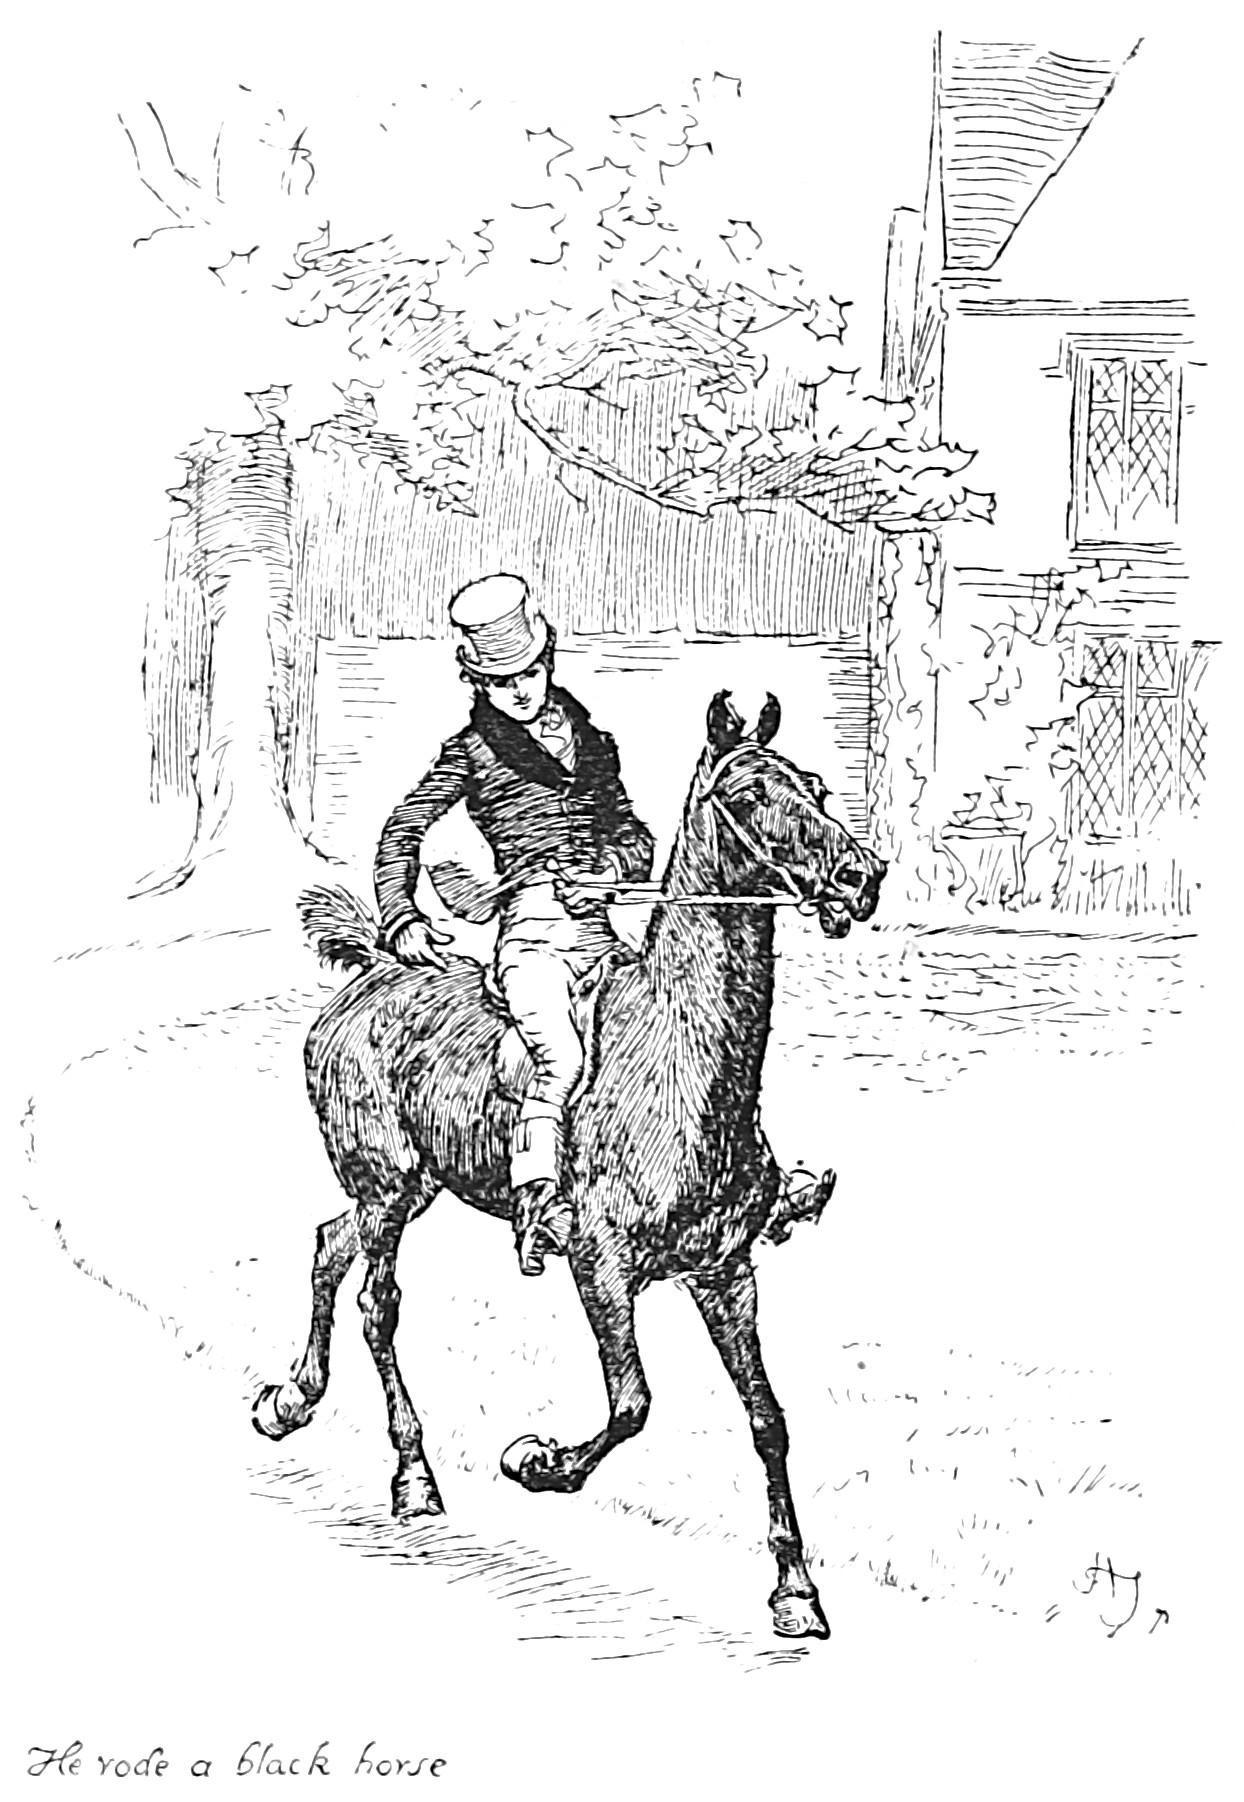
\includegraphics[width=.7\linewidth]{3blackhorse}
		\captionlistentry{He rode a black horse}
	\end{figure}


\lettrine[lines=6,image=true]{initials/chap3n}{ot} all that Mrs Bennet, however, with the assistance of her five daughters, could ask on the subject, was sufficient to draw from her husband any satisfactory description of Mr Bingley. They attacked him in various ways, with barefaced questions, ingenious suppositions, and distant surmises; but he eluded the skill of them all; and they were at last obliged to accept the second-hand intelligence of their neighbour, Lady Lucas. Her report was highly favourable. Sir William had been delighted with him. He was quite young, wonderfully handsome, extremely agreeable, and, to crown the whole, he meant to be at the next assembly with a large party. Nothing could be more delightful! To be fond of dancing was a certain step towards falling in love; and very lively hopes of Mr Bingley's heart were entertained.

<If I can but see one of my daughters happily settled at Netherfield,> said Mrs Bennet to her husband, <and all the others equally well married, I shall have nothing to wish for.>

In a few days Mr Bingley returned Mr Bennet's visit, and sat about ten minutes with him in his library. He had entertained hopes of being admitted to a sight of the young ladies, of whose beauty he had heard much; but he saw only the father. The ladies were somewhat more fortunate, for they had the advantage of ascertaining, from an upper window, that he wore a blue coat and rode a black horse.

\begin{figure}[tbh]
\centering
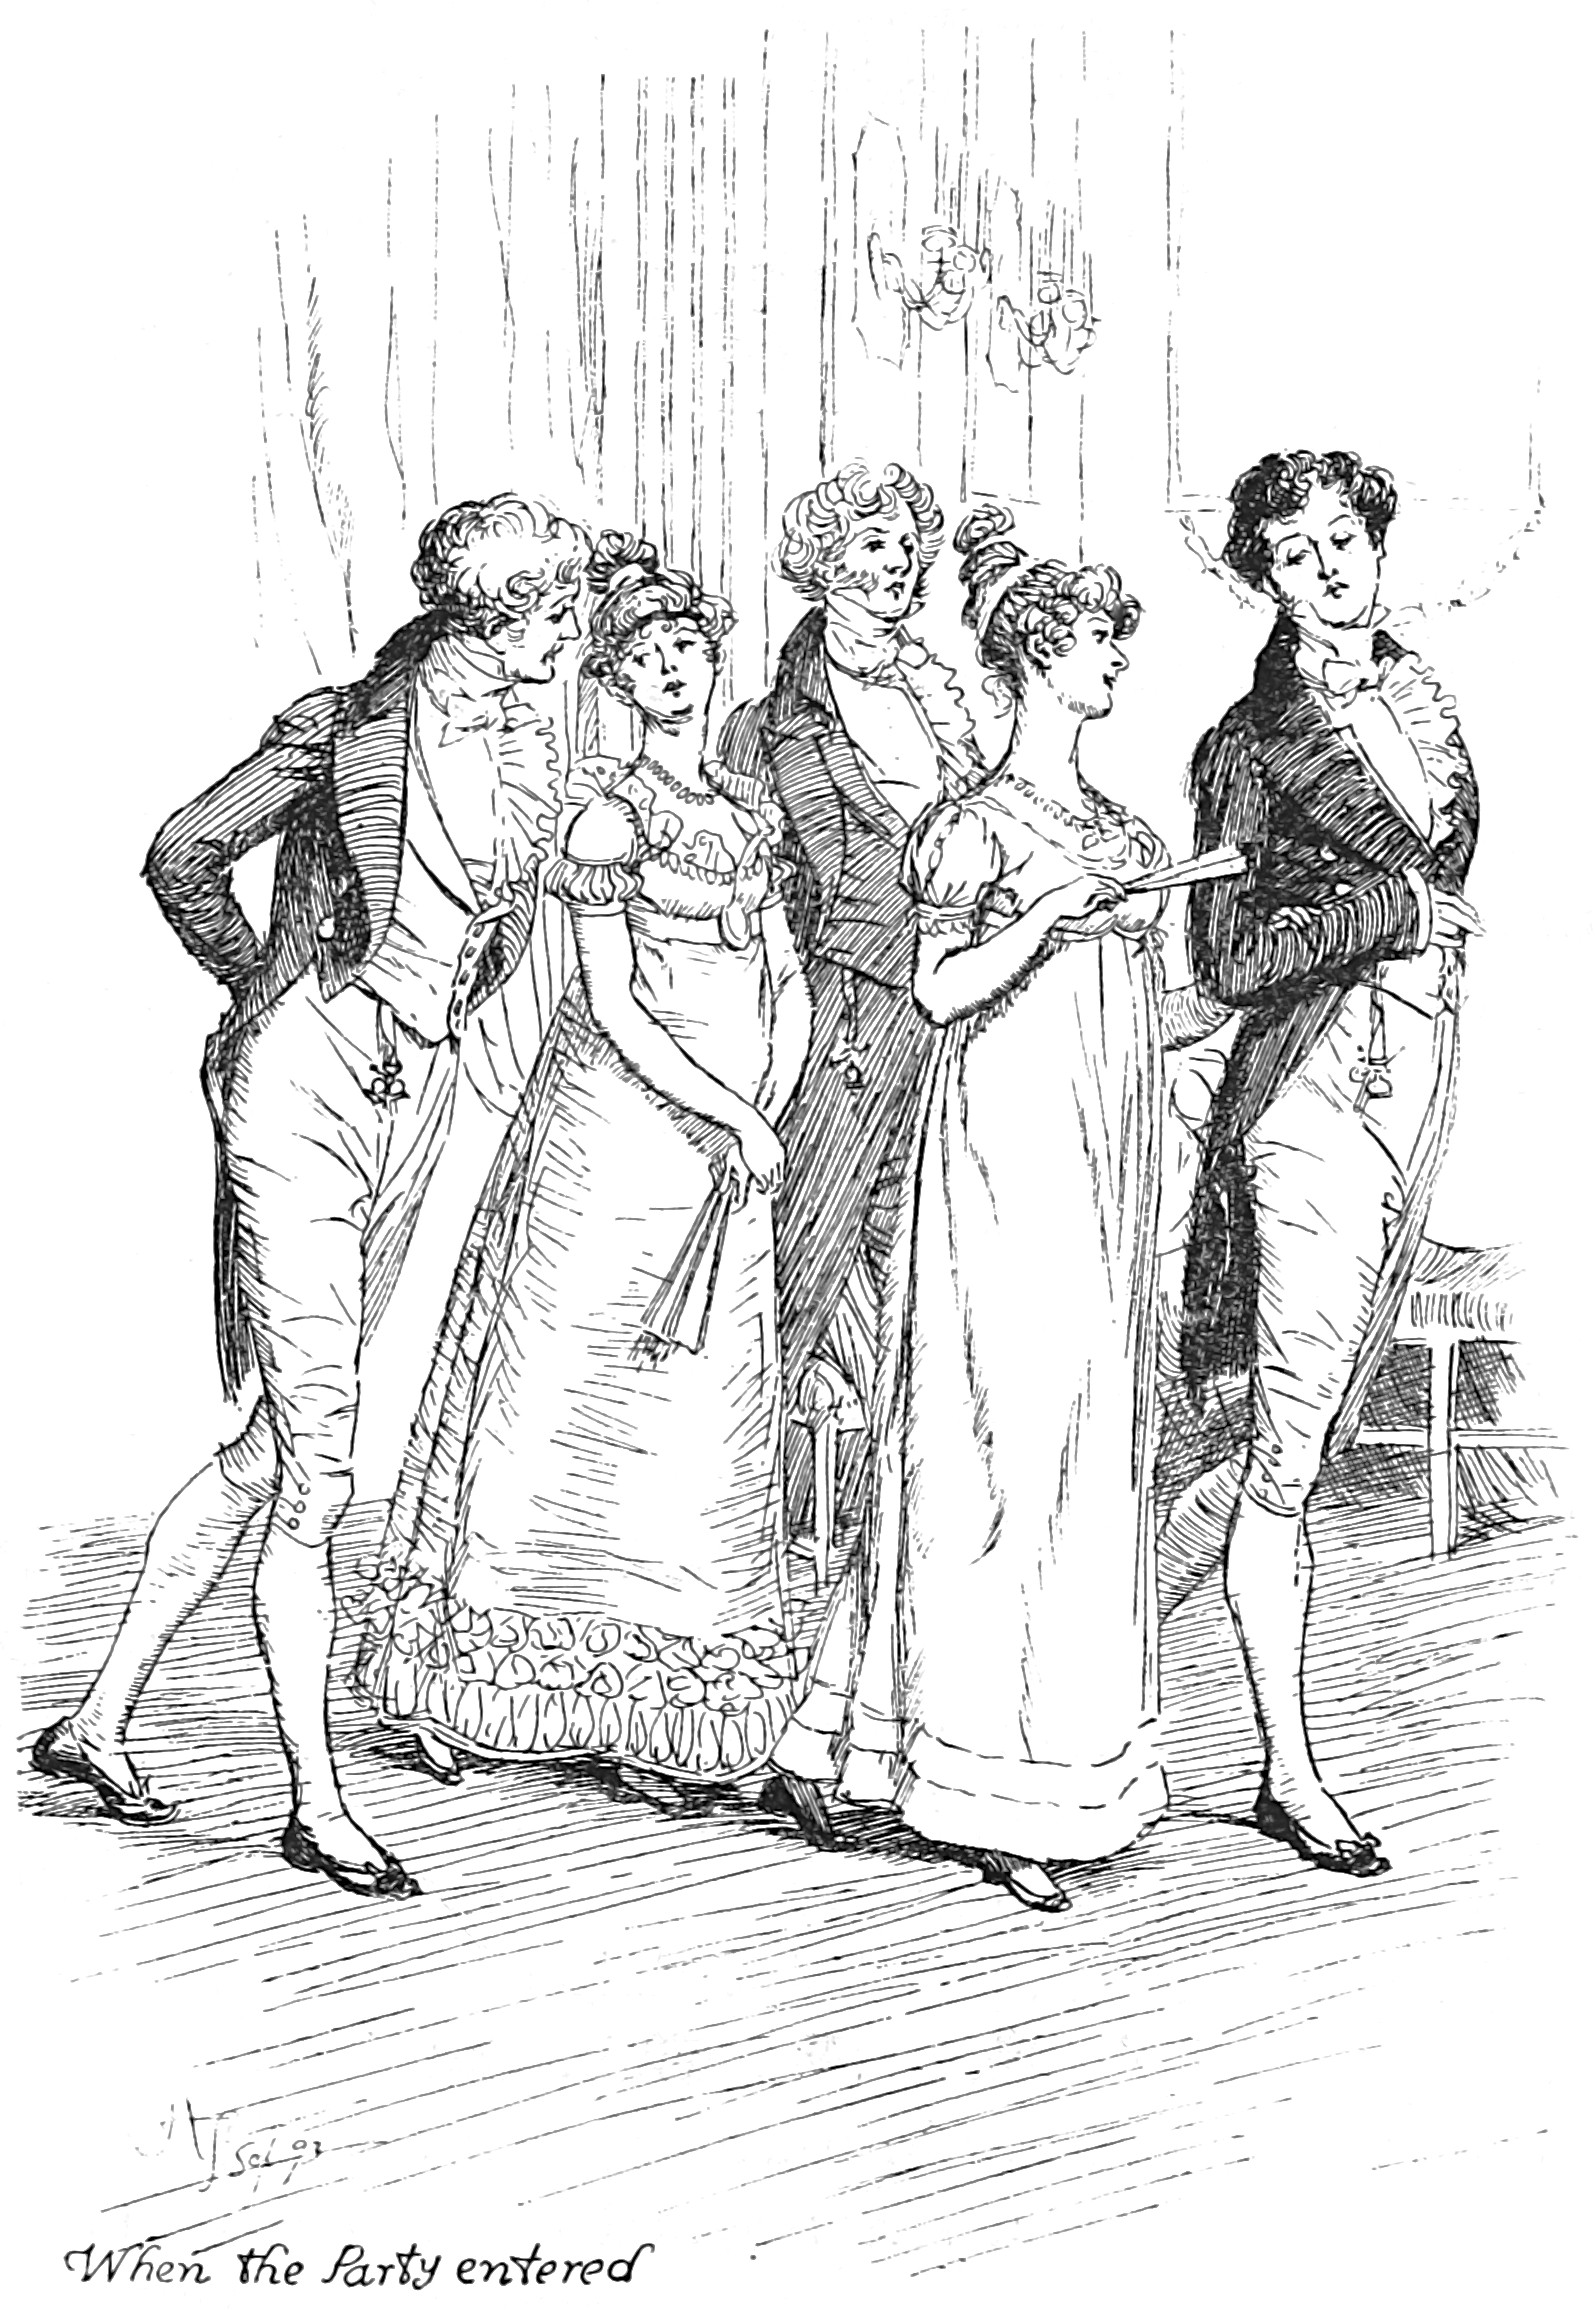
\includegraphics[width=.7\linewidth]{3partyentered}
\captionlistentry{When the party entered}
\end{figure}

An invitation to dinner was soon afterwards despatched; and already had Mrs Bennet planned the courses that were to do credit to her housekeeping, when an answer arrived which deferred it all. Mr Bingley was obliged to be in town the following day, and consequently unable to accept the honour of their invitation, etc. Mrs Bennet was quite disconcerted. She could not imagine what business he could have in town so soon after his arrival in Hertfordshire; and she began to fear that he might always be flying about from one place to another, and never settled at Netherfield as he ought to be. Lady Lucas quieted her fears a little by starting the idea of his being gone to London only to get a large party for the ball; and a report soon followed that Mr Bingley was to bring twelve ladies and seven gentlemen with him to the assembly. The girls grieved over such a number of ladies; but were comforted the day before the ball by hearing that, instead of twelve, he had brought only six with him from London, his five sisters and a cousin. And when the party entered the assembly-room, it consisted of only five altogether: Mr Bingley, his two sisters, the husband of the eldest, and another young man.

Mr Bingley was good-looking and gentlemanlike: he had a pleasant countenance, and easy, unaffected manners. His sisters were fine women, with an air of decided fashion. His brother-in-law, Mr Hurst, merely looked the gentleman; but his friend Mr Darcy soon drew the attention of the room by his fine, tall person, handsome features, noble mien, and the report, which was in general circulation within five minutes after his entrance, of his having ten thousand a year. The gentlemen pronounced him to be a fine figure of a man, the ladies declared he was much handsomer than Mr Bingley, and he was looked at with great admiration for about half the evening, till his manners gave a disgust which turned the tide of his popularity; for he was discovered to be proud, to be above his company, and above being pleased; and not all his large estate in Derbyshire could save him from having a most forbidding, disagreeable countenance, and being unworthy to be compared with his friend.

Mr Bingley had soon made himself acquainted with all the principal people in the room: he was lively and unreserved, danced every dance, was angry that the ball closed so early, and talked of giving one himself at Netherfield. Such amiable qualities must speak for themselves. What a contrast between him and his friend! Mr Darcy danced only once with Mrs Hurst and once with Miss Bingley, declined being introduced to any other lady, and spent the rest of the evening in walking about the room, speaking occasionally to one of his own party. His character was decided. He was the proudest, most disagreeable man in the world, and everybody hoped that he would never come there again. Amongst the most violent against him was Mrs Bennet, whose dislike of his general behaviour was sharpened into particular resentment by his having slighted one of her daughters.



Elizabeth Bennet had been obliged, by the scarcity of gentlemen, to sit down for two dances; and during part of that time, Mr Darcy had been standing near enough for her to overhear a conversation between him and Mr Bingley, who came from the dance for a few minutes to press his friend to join it.

<Come, Darcy,> said he, <I must have you dance. I hate to see you standing about by yourself in this stupid manner. You had much better dance.>

<I certainly shall not. You know how I detest it, unless I am particularly acquainted with my partner. At such an assembly as this, it would be insupportable. Your sisters are engaged, and there is not another woman in the room whom it would not be a punishment to me to stand up with.>

<I would not be so fastidious as you are,> cried Bingley, <for a kingdom! Upon my honour, I never met with so many pleasant girls in my life as I have this evening; and there are several of them, you see, uncommonly pretty.>

<\textit{You} are dancing with the only handsome girl in the room,> said Mr Darcy, looking at the eldest Miss Bennet.

<Oh, she is the most beautiful creature I ever beheld! But there is one of her sisters sitting down just behind you, who is very pretty, and I dare say very agreeable. Do let me ask my partner to introduce you.>

\begin{figure}[tbh]
\centering
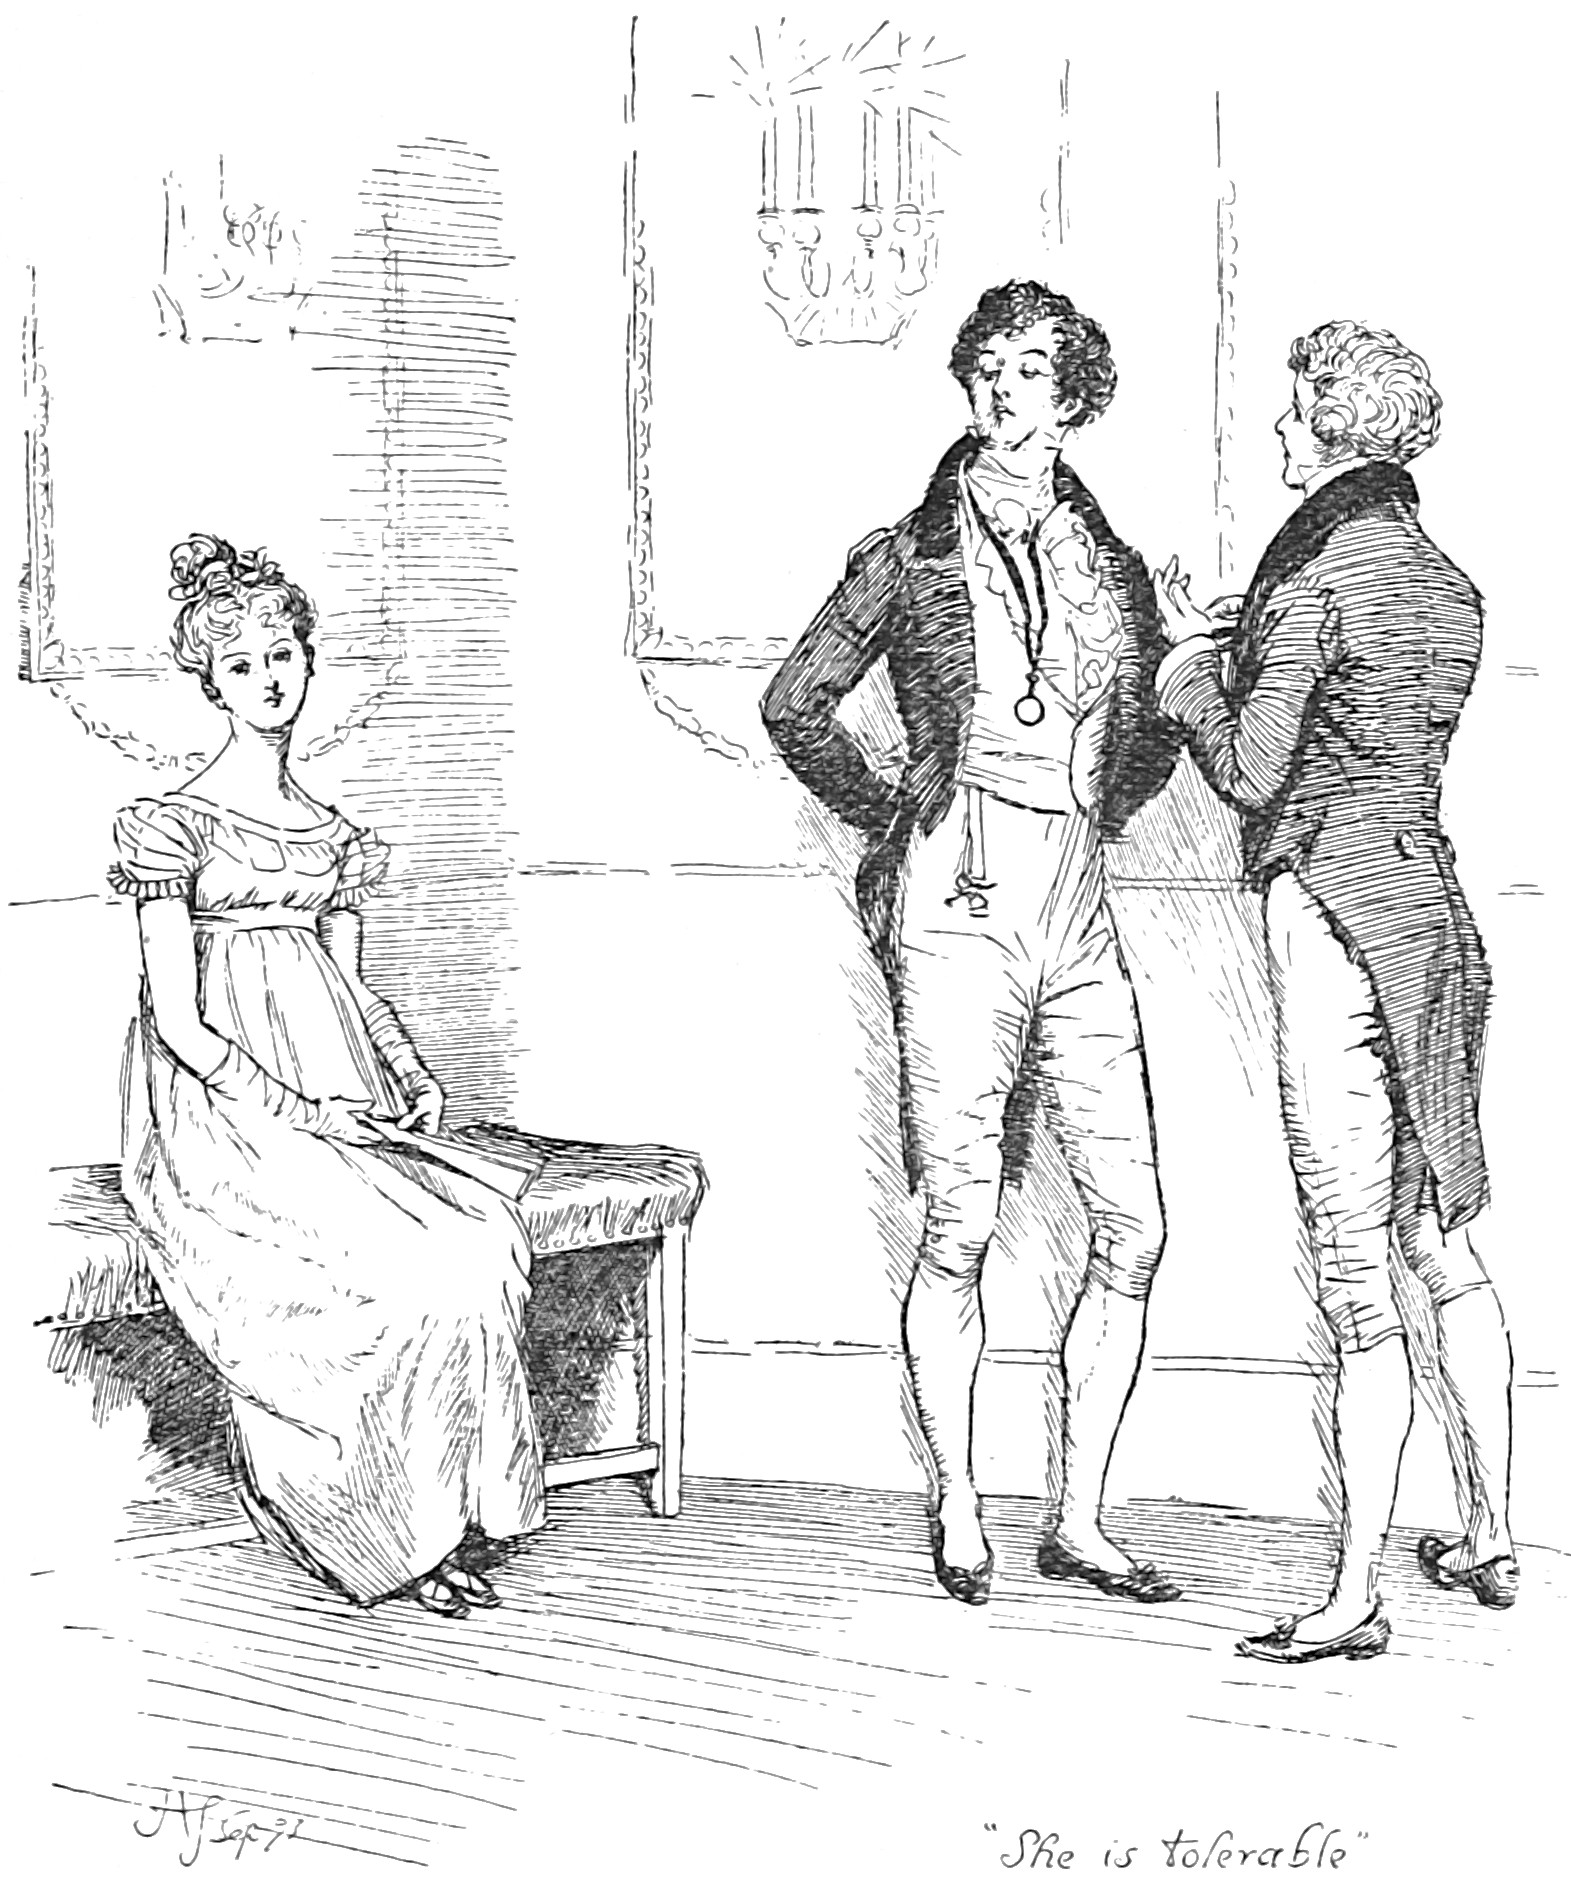
\includegraphics[width=.8\linewidth]{3tolerable}
\captionlistentry{<She is tolerable>}
\end{figure}

<Which do you mean?> and turning round, he looked for a moment at Elizabeth, till, catching her eye, he withdrew his own, and coldly said, <She is tolerable: but not handsome enough to tempt \textit{me}; and I am in no humour at present to give consequence to young ladies who are slighted by other men. You had better return to your partner and enjoy her smiles, for you are wasting your time with me.>



Mr Bingley followed his advice. Mr Darcy walked off; and Elizabeth remained with no very cordial feelings towards him. She told the story, however, with great spirit among her friends; for she had a lively, playful disposition, which delighted in anything ridiculous.

The evening altogether passed off pleasantly to the whole family. Mrs Bennet had seen her eldest daughter much admired by the Netherfield party. Mr Bingley had danced with her twice, and she had been distinguished by his sisters. Jane was as much gratified by this as her mother could be, though in a quieter way. Elizabeth felt Jane's pleasure. Mary had heard herself mentioned to Miss Bingley as the most accomplished girl in the neighbourhood; and Catherine and Lydia had been fortunate enough to be never without partners, which was all that they had yet learnt to care for at a ball. They returned, therefore, in good spirits to Longbourn, the village where they lived, and of which they were the principal inhabitants. They found Mr Bennet still up. With a book, he was regardless of time; and on the present occasion he had a good deal of curiosity as to the event of an evening which had raised such splendid expectations. He had rather hoped that all his wife's views on the stranger would be disappointed; but he soon found that he had a very different story to hear.

<Oh, my dear Mr Bennet,> as she entered the room, <we have had a most delightful evening, a most excellent ball. I wish you had been there. Jane was so admired, nothing could be like it. Everybody said how well she looked; and Mr Bingley thought her quite beautiful, and danced with her twice. Only think of \textit{that}, my dear: he actually danced with her twice; and she was the only creature in the room that he asked a second time. First of all, he asked Miss Lucas. I was so vexed to see him stand up with her; but, however, he did not admire her at all; indeed, nobody can, you know; and he seemed quite struck with Jane as she was going down the dance. So he inquired who she was, and got introduced, and asked her for the two next. Then, the two third he danced with Miss King, and the two fourth with Maria Lucas, and the two fifth with Jane again, and the two sixth with Lizzy, and the \textit{Boulanger}\longdash>

<If he had had any compassion for \textit{me},> cried her husband impatiently, <he would not have danced half so much! For God's sake, say no more of his partners. O that he had sprained his ancle in the first dance!>

<Oh, my dear,> continued Mrs Bennet, <I am quite delighted with him. He is so excessively handsome! and his sisters are charming women. I never in my life saw anything more elegant than their dresses. I dare say the lace upon Mrs Hurst's gown\longdash>

Here she was interrupted again. Mr Bennet protested against any description of finery. She was therefore obliged to seek another branch of the subject, and related, with much bitterness of spirit, and some exaggeration, the shocking rudeness of Mr Darcy.

<But I can assure you,> she added, <that Lizzy does not lose much by not suiting \textit{his} fancy; for he is a most disagreeable, horrid man, not at all worth pleasing. So high and so conceited, that there was no enduring him! He walked here, and he walked there, fancying himself so very great! Not handsome enough to dance with! I wish you had been there, my dear, to have given him one of your set-downs. I quite detest the man.>

%!TeX root=../emmatop.tex
\chapter[Chapter \thechapter]{}
\lettrine[lines=4,lraise=0.3]{H}{arriet} Smith's intimacy at Hartfield was soon a settled thing. Quick and decided in her ways, Emma lost no time in inviting, encouraging, and telling her to come very often; and as their acquaintance increased, so did their satisfaction in each other. As a walking companion, Emma had very early foreseen how useful she might find her. In that respect Mrs Weston's loss had been important. Her father never went beyond the shrubbery, where two divisions of the ground sufficed him for his long walk, or his short, as the year varied; and since Mrs Weston's marriage her exercise had been too much confined. She had ventured once alone to Randalls, but it was not pleasant; and a Harriet Smith, therefore, one whom she could summon at any time to a walk, would be a valuable addition to her privileges. But in every respect, as she saw more of her, she approved her, and was confirmed in all her kind designs.

Harriet certainly was not clever, but she had a sweet, docile, grateful disposition, was totally free from conceit, and only desiring to be guided by any one she looked up to. Her early attachment to herself was very amiable; and her inclination for good company, and power of appreciating what was elegant and clever, shewed that there was no want of taste, though strength of understanding must not be expected. Altogether she was quite convinced of Harriet Smith's being exactly the young friend she wanted—exactly the something which her home required. Such a friend as Mrs Weston was out of the question. Two such could never be granted. Two such she did not want. It was quite a different sort of thing, a sentiment distinct and independent. Mrs Weston was the object of a regard which had its basis in gratitude and esteem. Harriet would be loved as one to whom she could be useful. For Mrs Weston there was nothing to be done; for Harriet every thing.

Her first attempts at usefulness were in an endeavour to find out who were the parents, but Harriet could not tell. She was ready to tell every thing in her power, but on this subject questions were vain. Emma was obliged to fancy what she liked—but she could never believe that in the same situation \textit{she} should not have discovered the truth. Harriet had no penetration. She had been satisfied to hear and believe just what Mrs Goddard chose to tell her; and looked no farther.

Mrs Goddard, and the teachers, and the girls and the affairs of the school in general, formed naturally a great part of the conversation—and but for her acquaintance with the Martins of Abbey-Mill Farm, it must have been the whole. But the Martins occupied her thoughts a good deal; she had spent two very happy months with them, and now loved to talk of the pleasures of her visit, and describe the many comforts and wonders of the place. Emma encouraged her talkativeness—amused by such a picture of another set of beings, and enjoying the youthful simplicity which could speak with so much exultation of Mrs Martin's having »\textit{two} parlours, two very good parlours, indeed; one of them quite as large as Mrs Goddard's drawing-room; and of her having an upper maid who had lived five-and-twenty years with her; and of their having eight cows, two of them Alderneys, and one a little Welch cow, a very pretty little Welch cow indeed; and of Mrs Martin's saying as she was so fond of it, it should be called \textit{her} cow; and of their having a very handsome summer-house in their garden, where some day next year they were all to drink tea:—a very handsome summer-house, large enough to hold a dozen people.«

For some time she was amused, without thinking beyond the immediate cause; but as she came to understand the family better, other feelings arose. She had taken up a wrong idea, fancying it was a mother and daughter, a son and son's wife, who all lived together; but when it appeared that the Mr Martin, who bore a part in the narrative, and was always mentioned with approbation for his great good-nature in doing something or other, was a single man; that there was no young Mrs Martin, no wife in the case; she did suspect danger to her poor little friend from all this hospitality and kindness, and that, if she were not taken care of, she might be required to sink herself forever.

With this inspiriting notion, her questions increased in number and meaning; and she particularly led Harriet to talk more of Mr Martin, and there was evidently no dislike to it. Harriet was very ready to speak of the share he had had in their moonlight walks and merry evening games; and dwelt a good deal upon his being so very good-humoured and obliging. He had gone three miles round one day in order to bring her some walnuts, because she had said how fond she was of them, and in every thing else he was so very obliging. He had his shepherd's son into the parlour one night on purpose to sing to her. She was very fond of singing. He could sing a little himself. She believed he was very clever, and understood every thing. He had a very fine flock, and, while she was with them, he had been bid more for his wool than any body in the country. She believed every body spoke well of him. His mother and sisters were very fond of him. Mrs Martin had told her one day (and there was a blush as she said it,) that it was impossible for any body to be a better son, and therefore she was sure, whenever he married, he would make a good husband. Not that she \textit{wanted} him to marry. She was in no hurry at all.

»Well done, Mrs Martin!« thought Emma. »You know what you are about.«

»And when she had come away, Mrs Martin was so very kind as to send Mrs Goddard a beautiful goose—the finest goose Mrs Goddard had ever seen. Mrs Goddard had dressed it on a Sunday, and asked all the three teachers, Miss Nash, and Miss Prince, and Miss Richardson, to sup with her.«

»Mr Martin, I suppose, is not a man of information beyond the line of his own business? He does not read?«

»Oh yes!—that is, no—I do not know—but I believe he has read a good deal—but not what you would think any thing of. He reads the \textit{Agricultural Reports}, and some other books that lay in one of the window seats—but he reads all \textit{them} to himself. But sometimes of an evening, before we went to cards, he would read something aloud out of the \textit{Elegant Extracts}, very entertaining. And I know he has read \textit{The Vicar of Wakefield}. He never read \textit{The Romance of the Forest}, nor \textit{The Children of the Abbey}. He had never heard of such books before I mentioned them, but he is determined to get them now as soon as ever he can.«

The next question was—

»What sort of looking man is Mr Martin?«

»Oh! not handsome—not at all handsome. I thought him very plain at first, but I do not think him so plain now. One does not, you know, after a time. But did you never see him? He is in Highbury every now and then, and he is sure to ride through every week in his way to Kingston. He has passed you very often.«

»That may be, and I may have seen him fifty times, but without having any idea of his name. A young farmer, whether on horseback or on foot, is the very last sort of person to raise my curiosity. The yeomanry are precisely the order of people with whom I feel I can have nothing to do. A degree or two lower, and a creditable appearance might interest me; I might hope to be useful to their families in some way or other. But a farmer can need none of my help, and is, therefore, in one sense, as much above my notice as in every other he is below it.«

»To be sure. Oh yes! It is not likely you should ever have observed him; but he knows you very well indeed—I mean by sight.«

»I have no doubt of his being a very respectable young man. I know, indeed, that he is so, and, as such, wish him well. What do you imagine his age to be?«

»He was four-and-twenty the 8th of last June, and my birthday is the 23rd just a fortnight and a day's difference—which is very odd.«

»Only four-and-twenty. That is too young to settle. His mother is perfectly right not to be in a hurry. They seem very comfortable as they are, and if she were to take any pains to marry him, she would probably repent it. Six years hence, if he could meet with a good sort of young woman in the same rank as his own, with a little money, it might be very desirable.«

»Six years hence! Dear Miss Woodhouse, he would be thirty years old!«

»Well, and that is as early as most men can afford to marry, who are not born to an independence. Mr Martin, I imagine, has his fortune entirely to make—cannot be at all beforehand with the world. Whatever money he might come into when his father died, whatever his share of the family property, it is, I dare say, all afloat, all employed in his stock, and so forth; and though, with diligence and good luck, he may be rich in time, it is next to impossible that he should have realised any thing yet.«

»To be sure, so it is. But they live very comfortably. They have no indoors man, else they do not want for any thing; and Mrs Martin talks of taking a boy another year.«

»I wish you may not get into a scrape, Harriet, whenever he does marry;—I mean, as to being acquainted with his wife—for though his sisters, from a superior education, are not to be altogether objected to, it does not follow that he might marry any body at all fit for you to notice. The misfortune of your birth ought to make you particularly careful as to your associates. There can be no doubt of your being a gentleman's daughter, and you must support your claim to that station by every thing within your own power, or there will be plenty of people who would take pleasure in degrading you.«

»Yes, to be sure, I suppose there are. But while I visit at Hartfield, and you are so kind to me, Miss Woodhouse, I am not afraid of what any body can do.«

»You understand the force of influence pretty well, Harriet; but I would have you so firmly established in good society, as to be independent even of Hartfield and Miss Woodhouse. I want to see you permanently well connected, and to that end it will be advisable to have as few odd acquaintance as may be; and, therefore, I say that if you should still be in this country when Mr Martin marries, I wish you may not be drawn in by your intimacy with the sisters, to be acquainted with the wife, who will probably be some mere farmer's daughter, without education.«

»To be sure. Yes. Not that I think Mr Martin would ever marry any body but what had had some education—and been very well brought up. However, I do not mean to set up my opinion against yours—and I am sure I shall not wish for the acquaintance of his wife. I shall always have a great regard for the Miss Martins, especially Elizabeth, and should be very sorry to give them up, for they are quite as well educated as me. But if he marries a very ignorant, vulgar woman, certainly I had better not visit her, if I can help it.«

Emma watched her through the fluctuations of this speech, and saw no alarming symptoms of love. The young man had been the first admirer, but she trusted there was no other hold, and that there would be no serious difficulty, on Harriet's side, to oppose any friendly arrangement of her own.

\begin{figure}[tbph]
\centering

\includegraphics[width=.8\linewidth]{4notsorry}
\caption{Emma was not sorry to have such an opportunity of survey}
\end{figure}

They met Mr Martin the very next day, as they were walking on the Donwell road. He was on foot, and after looking very respectfully at her, looked with most unfeigned satisfaction at her companion. Emma was not sorry to have such an opportunity of survey; and walking a few yards forward, while they talked together, soon made her quick eye sufficiently acquainted with Mr Robert Martin. His appearance was very neat, and he looked like a sensible young man, but his person had no other advantage; and when he came to be contrasted with gentlemen, she thought he must lose all the ground he had gained in Harriet's inclination. Harriet was not insensible of manner; she had voluntarily noticed her father's gentleness with admiration as well as wonder. Mr Martin looked as if he did not know what manner was.

They remained but a few minutes together, as Miss Woodhouse must not be kept waiting; and Harriet then came running to her with a smiling face, and in a flutter of spirits, which Miss Woodhouse hoped very soon to compose.

»Only think of our happening to meet him!—How very odd! It was quite a chance, he said, that he had not gone round by Randalls. He did not think we ever walked this road. He thought we walked towards Randalls most days. He has not been able to get the Romance of the Forest yet. He was so busy the last time he was at Kingston that he quite forgot it, but he goes again to-morrow. So very odd we should happen to meet! Well, Miss Woodhouse, is he like what you expected? What do you think of him? Do you think him so very plain?«

»He is very plain, undoubtedly—remarkably plain:—but that is nothing compared with his entire want of gentility. I had no right to expect much, and I did not expect much; but I had no idea that he could be so very clownish, so totally without air. I had imagined him, I confess, a degree or two nearer gentility.«

»To be sure,« said Harriet, in a mortified voice, »he is not so genteel as real gentlemen.«

»I think, Harriet, since your acquaintance with us, you have been repeatedly in the company of some such very real gentlemen, that you must yourself be struck with the difference in Mr Martin. At Hartfield, you have had very good specimens of well educated, well bred men. I should be surprized if, after seeing them, you could be in company with Mr Martin again without perceiving him to be a very inferior creature—and rather wondering at yourself for having ever thought him at all agreeable before. Do not you begin to feel that now? Were not you struck? I am sure you must have been struck by his awkward look and abrupt manner, and the uncouthness of a voice which I heard to be wholly unmodulated as I stood here.«

»Certainly, he is not like Mr Knightley. He has not such a fine air and way of walking as Mr Knightley. I see the difference plain enough. But Mr Knightley is so very fine a man!«

»Mr Knightley's air is so remarkably good that it is not fair to compare Mr Martin with \textit{him}. You might not see one in a hundred with \textit{gentleman} so plainly written as in Mr Knightley. But he is not the only gentleman you have been lately used to. What say you to Mr Weston and Mr Elton? Compare Mr Martin with either of \textit{them}. Compare their manner of carrying themselves; of walking; of speaking; of being silent. You must see the difference.«

»Oh yes!—there is a great difference. But Mr Weston is almost an old man. Mr Weston must be between forty and fifty.«

»Which makes his good manners the more valuable. The older a person grows, Harriet, the more important it is that their manners should not be bad; the more glaring and disgusting any loudness, or coarseness, or awkwardness becomes. What is passable in youth is detestable in later age. Mr Martin is now awkward and abrupt; what will he be at Mr Weston's time of life?«

»There is no saying, indeed,« replied Harriet rather solemnly.

»But there may be pretty good guessing. He will be a completely gross, vulgar farmer, totally inattentive to appearances, and thinking of nothing but profit and loss.«

»Will he, indeed? That will be very bad.«

»How much his business engrosses him already is very plain from the circumstance of his forgetting to inquire for the book you recommended. He was a great deal too full of the market to think of any thing else—which is just as it should be, for a thriving man. What has he to do with books? And I have no doubt that he \textit{will} thrive, and be a very rich man in time—and his being illiterate and coarse need not disturb \textit{us}.«

»I wonder he did not remember the book«—was all Harriet's answer, and spoken with a degree of grave displeasure which Emma thought might be safely left to itself. She, therefore, said no more for some time. Her next beginning was,

»In one respect, perhaps, Mr Elton's manners are superior to Mr Knightley's or Mr Weston's. They have more gentleness. They might be more safely held up as a pattern. There is an openness, a quickness, almost a bluntness in Mr Weston, which every body likes in \textit{him}, because there is so much good-humour with it—but that would not do to be copied. Neither would Mr Knightley's downright, decided, commanding sort of manner, though it suits \textit{him} very well; his figure, and look, and situation in life seem to allow it; but if any young man were to set about copying him, he would not be sufferable. On the contrary, I think a young man might be very safely recommended to take Mr Elton as a model. Mr Elton is good-humoured, cheerful, obliging, and gentle. He seems to me to be grown particularly gentle of late. I do not know whether he has any design of ingratiating himself with either of us, Harriet, by additional softness, but it strikes me that his manners are softer than they used to be. If he means any thing, it must be to please you. Did not I tell you what he said of you the other day?«

She then repeated some warm personal praise which she had drawn from Mr Elton, and now did full justice to; and Harriet blushed and smiled, and said she had always thought Mr Elton very agreeable.

Mr Elton was the very person fixed on by Emma for driving the young farmer out of Harriet's head. She thought it would be an excellent match; and only too palpably desirable, natural, and probable, for her to have much merit in planning it. She feared it was what every body else must think of and predict. It was not likely, however, that any body should have equalled her in the date of the plan, as it had entered her brain during the very first evening of Harriet's coming to Hartfield. The longer she considered it, the greater was her sense of its expediency. Mr Elton's situation was most suitable, quite the gentleman himself, and without low connexions; at the same time, not of any family that could fairly object to the doubtful birth of Harriet. He had a comfortable home for her, and Emma imagined a very sufficient income; for though the vicarage of Highbury was not large, he was known to have some independent property; and she thought very highly of him as a good-humoured, well-meaning, respectable young man, without any deficiency of useful understanding or knowledge of the world.

She had already satisfied herself that he thought Harriet a beautiful girl, which she trusted, with such frequent meetings at Hartfield, was foundation enough on his side; and on Harriet's there could be little doubt that the idea of being preferred by him would have all the usual weight and efficacy. And he was really a very pleasing young man, a young man whom any woman not fastidious might like. He was reckoned very handsome; his person much admired in general, though not by her, there being a want of elegance of feature which she could not dispense with:—but the girl who could be gratified by a Robert Martin's riding about the country to get walnuts for her might very well be conquered by Mr Elton's admiration.
\chapter[Chapter \thechapter]{} 

 \lettrine[lraise=0.3]{T}{he} young people were pleased with each other from the first. On each side there was much to attract, and their acquaintance soon promised as early an intimacy as good manners would warrant. Miss~Crawford's beauty did her no disservice with the Miss~Bertrams. They were too handsome themselves to dislike any woman for being so too, and were almost as much charmed as their brothers with her lively dark eye, clear brown complexion, and general prettiness. Had she been tall, full formed, and fair, it might have been more of a trial: but as it was, there could be no comparison; and she was most allowably a sweet, pretty girl, while they were the finest young women in the country.

Her brother was not handsome: no, when they first saw him he was absolutely plain, black and plain; but still he was the gentleman, with a pleasing address. The second meeting proved him not so very plain: he was plain, to be sure, but then he had so much countenance, and his teeth were so good, and he was so well made, that one soon forgot he was plain; and after a third interview, after dining in company with him at the Parsonage, he was no longer allowed to be called so by anybody. He was, in fact, the most agreeable young man the sisters had ever known, and they were equally delighted with him. Miss~Bertram's engagement made him in equity the property of Julia, of which Julia was fully aware; and before he had been at Mansfield a week, she was quite ready to be fallen in love with.

Maria's notions on the subject were more confused and indistinct. She did not want to see or understand. <There could be no harm in her liking an agreeable man—everybody knew her situation—Mr~Crawford must take care of himself.> Mr~Crawford did not mean to be in any danger! the Miss~Bertrams were worth pleasing, and were ready to be pleased; and he began with no object but of making them like him. He did not want them to die of love; but with sense and temper which ought to have made him judge and feel better, he allowed himself great latitude on such points.

<I like your Miss~Bertrams exceedingly, sister,> said he, as he returned from attending them to their carriage after the said dinner visit; <they are very elegant, agreeable girls.>

<So they are indeed, and I am delighted to hear you say it. But you like Julia best.>

<Oh yes! I like Julia best.>

<But do you really? for Miss~Bertram is in general thought the handsomest.>

<So I should suppose. She has the advantage in every feature, and I prefer her countenance; but I like Julia best; Miss~Bertram is certainly the handsomest, and I have found her the most agreeable, but I shall always like Julia best, because you order me.>

<I shall not talk to you, Henry, but I know you \textit{will}  like her best at last.>

<Do not I tell you that I like her best \textit{at first}?>

<And besides, Miss~Bertram is engaged. Remember that, my dear brother. Her choice is made.>

<Yes, and I like her the better for it. An engaged woman is always more agreeable than a disengaged. She is satisfied with herself. Her cares are over, and she feels that she may exert all her powers of pleasing without suspicion. All is safe with a lady engaged: no harm can be done.>

<Why, as to that, Mr~Rushworth is a very good sort of young man, and it is a great match for her.>

<But Miss~Bertram does not care three straws for him; \textit{that}  is your opinion of your intimate friend. \textit{I}  do not subscribe to it. I am sure Miss~Bertram is very much attached to Mr~Rushworth. I could see it in her eyes, when he was mentioned. I think too well of Miss~Bertram to suppose she would ever give her hand without her heart.>

<Mary, how shall we manage him?>

<We must leave him to himself, I believe. Talking does no good. He will be taken in at last.>

<But I would not have him \textit{taken in}; I would not have him duped; I would have it all fair and honourable.>

<Oh dear! let him stand his chance and be taken in. It will do just as well. Everybody is taken in at some period or other.>

<Not always in marriage, dear Mary.>

<In marriage especially. With all due respect to such of the present company as chance to be married, my dear Mrs~Grant, there is not one in a hundred of either sex who is not taken in when they marry. Look where I will, I see that it \textit{is}  so; and I feel that it \textit{must}  be so, when I consider that it is, of all transactions, the one in which people expect most from others, and are least honest themselves.>

<Ah! You have been in a bad school for matrimony, in Hill Street.>

<My poor aunt had certainly little cause to love the state; but, however, speaking from my own observation, it is a manoeuvring business. I know so many who have married in the full expectation and confidence of some one particular advantage in the connexion, or accomplishment, or good quality in the person, who have found themselves entirely deceived, and been obliged to put up with exactly the reverse. What is this but a take in?>

<My dear child, there must be a little imagination here. I beg your pardon, but I cannot quite believe you. Depend upon it, you see but half. You see the evil, but you do not see the consolation. There will be little rubs and disappointments everywhere, and we are all apt to expect too much; but then, if one scheme of happiness fails, human nature turns to another; if the first calculation is wrong, we make a second better: we find comfort somewhere—and those evil-minded observers, dearest Mary, who make much of a little, are more taken in and deceived than the parties themselves.>

<Well done, sister! I honour your \textit{esprit du corps}. When I am a wife, I mean to be just as staunch myself; and I wish my friends in general would be so too. It would save me many a heartache.>

<You are as bad as your brother, Mary; but we will cure you both. Mansfield shall cure you both, and without any taking in. Stay with us, and we will cure you.>

The Crawfords, without wanting to be cured, were very willing to stay. Mary was satisfied with the Parsonage as a present home, and Henry equally ready to lengthen his visit. He had come, intending to spend only a few days with them; but Mansfield promised well, and there was nothing to call him elsewhere. It delighted Mrs~Grant to keep them both with her, and Dr~Grant was exceedingly well contented to have it so: a talking pretty young woman like Miss~Crawford is always pleasant society to an indolent, stay-at-home man; and Mr~Crawford's being his guest was an excuse for drinking claret every day.

The Miss~Bertrams' admiration of Mr~Crawford was more rapturous than anything which Miss~Crawford's habits made her likely to feel. She acknowledged, however, that the Mr~Bertrams were very fine young men, that two such young men were not often seen together even in London, and that their manners, particularly those of the eldest, were very good. \textit{He}  had been much in London, and had more liveliness and gallantry than Edmund, and must, therefore, be preferred; and, indeed, his being the eldest was another strong claim. She had felt an early presentiment that she \textit{should}  like the eldest best. She knew it was her way.

Tom Bertram must have been thought pleasant, indeed, at any rate; he was the sort of young man to be generally liked, his agreeableness was of the kind to be oftener found agreeable than some endowments of a higher stamp, for he had easy manners, excellent spirits, a large acquaintance, and a great deal to say; and the reversion of Mansfield Park, and a baronetcy, did no harm to all this. Miss~Crawford soon felt that he and his situation might do. She looked about her with due consideration, and found almost everything in his favour: a park, a real park, five miles round, a spacious modern-built house, so well placed and well screened as to deserve to be in any collection of engravings of gentlemen's seats in the kingdom, and wanting only to be completely new furnished—pleasant sisters, a quiet mother, and an agreeable man himself—with the advantage of being tied up from much gaming at present by a promise to his father, and of being Sir~Thomas hereafter. It might do very well; she believed she should accept him; and she began accordingly to interest herself a little about the horse which he had to run at the B\doubleemdash races.

These races were to call him away not long after their acquaintance began; and as it appeared that the family did not, from his usual goings on, expect him back again for many weeks, it would bring his passion to an early proof. Much was said on his side to induce her to attend the races, and schemes were made for a large party to them, with all the eagerness of inclination, but it would only do to be talked of.

And Fanny, what was \textit{she}  doing and thinking all this while? and what was \textit{her}  opinion of the newcomers? Few young ladies of eighteen could be less called on to speak their opinion than Fanny. In a quiet way, very little attended to, she paid her tribute of admiration to Miss~Crawford's beauty; but as she still continued to think Mr~Crawford very plain, in spite of her two cousins having repeatedly proved the contrary, she never mentioned \textit{him}. The notice, which she excited herself, was to this effect. <I begin now to understand you all, except Miss~Price,> said Miss~Crawford, as she was walking with the Mr~Bertrams. <Pray, is she out, or is she not? I am puzzled. She dined at the Parsonage, with the rest of you, which seemed like being \textit{out}; and yet she says so little, that I can hardly suppose she \textit{is}.>

Edmund, to whom this was chiefly addressed, replied, <I believe I know what you mean, but I will not undertake to answer the question. My cousin is grown up. She has the age and sense of a woman, but the outs and not outs are beyond me.>

<And yet, in general, nothing can be more easily ascertained. The distinction is so broad. Manners as well as appearance are, generally speaking, so totally different. Till now, I could not have supposed it possible to be mistaken as to a girl's being out or not. A girl not out has always the same sort of dress: a close bonnet, for instance; looks very demure, and never says a word. You may smile, but it is so, I assure you; and except that it is sometimes carried a little too far, it is all very proper. Girls should be quiet and modest. The most objectionable part is, that the alteration of manners on being introduced into company is frequently too sudden. They sometimes pass in such very little time from reserve to quite the opposite—to confidence! \textit{That}  is the faulty part of the present system. One does not like to see a girl of eighteen or nineteen so immediately up to every thing—and perhaps when one has seen her hardly able to speak the year before. Mr~Bertram, I dare say \textit{you}  have sometimes met with such changes.>

<I believe I have, but this is hardly fair; I see what you are at. You are quizzing me and Miss~Anderson.>

<No, indeed. Miss~Anderson! I do not know who or what you mean. I am quite in the dark. But I \textit{will}  quiz you with a great deal of pleasure, if you will tell me what about.>

<Ah! you carry it off very well, but I cannot be quite so far imposed on. You must have had Miss~Anderson in your eye, in describing an altered young lady. You paint too accurately for mistake. It was exactly so. The Andersons of Baker Street. We were speaking of them the other day, you know. Edmund, you have heard me mention Charles Anderson. The circumstance was precisely as this lady has represented it. When Anderson first introduced me to his family, about two years ago, his sister was not \textit{out}, and I could not get her to speak to me. I sat there an hour one morning waiting for Anderson, with only her and a little girl or two in the room, the governess being sick or run away, and the mother in and out every moment with letters of business, and I could hardly get a word or a look from the young lady—nothing like a civil answer—she screwed up her mouth, and turned from me with such an air! I did not see her again for a twelvemonth. She was then \textit{out}. I met her at Mrs~Holford's, and did not recollect her. She came up to me, claimed me as an acquaintance, stared me out of countenance; and talked and laughed till I did not know which way to look. I felt that I must be the jest of the room at the time, and Miss~Crawford, it is plain, has heard the story.>

<And a very pretty story it is, and with more truth in it, I dare say, than does credit to Miss~Anderson. It is too common a fault. Mothers certainly have not yet got quite the right way of managing their daughters. I do not know where the error lies. I do not pretend to set people right, but I do see that they are often wrong.>

<Those who are showing the world what female manners \textit{should}  be,> said Mr~Bertram gallantly, <are doing a great deal to set them right.>

<The error is plain enough,> said the less courteous Edmund; <such girls are ill brought up. They are given wrong notions from the beginning. They are always acting upon motives of vanity, and there is no more real modesty in their behaviour \textit{before}  they appear in public than afterwards.>

<I do not know,> replied Miss~Crawford hesitatingly. <Yes, I cannot agree with you there. It is certainly the modestest part of the business. It is much worse to have girls not out give themselves the same airs and take the same liberties as if they were, which I have seen done. That is worse than anything—quite disgusting!>

<Yes, \textit{that}  is very inconvenient indeed,> said Mr~Bertram. <It leads one astray; one does not know what to do. The close bonnet and demure air you describe so well (and nothing was ever juster), tell one what is expected; but I got into a dreadful scrape last year from the want of them. I went down to Ramsgate for a week with a friend last September, just after my return from the West Indies. My friend Sneyd—you have heard me speak of Sneyd, Edmund—his father, and mother, and sisters, were there, all new to me. When we reached Albion Place they were out; we went after them, and found them on the pier: Mrs~and the two Miss~Sneyds, with others of their acquaintance. I made my bow in form; and as Mrs~Sneyd was surrounded by men, attached myself to one of her daughters, walked by her side all the way home, and made myself as agreeable as I could; the young lady perfectly easy in her manners, and as ready to talk as to listen. I had not a suspicion that I could be doing anything wrong. They looked just the same: both well-dressed, with veils and parasols like other girls; but I afterwards found that I had been giving all my attention to the youngest, who was not \textit{out}, and had most excessively offended the eldest. Miss~Augusta ought not to have been noticed for the next six months; and Miss~Sneyd, I believe, has never forgiven me.>

<That was bad indeed. Poor Miss~Sneyd. Though I have no younger sister, I feel for her. To be neglected before one's time must be very vexatious; but it was entirely the mother's fault. Miss~Augusta should have been with her governess. Such half-and-half doings never prosper. But now I must be satisfied about Miss~Price. Does she go to balls? Does she dine out every where, as well as at my sister's?>

<No,> replied Edmund; <I do not think she has ever been to a ball. My mother seldom goes into company herself, and dines nowhere but with Mrs~Grant, and Fanny stays at home with \textit{her}.>

<Oh! then the point is clear. Miss~Price is not out.> 
%!TeX root=../sensetop.tex
\chapter[Chapter \thechapter]{}
\lettrine[lraise=0.3]{T}{he} first part of their journey was performed in too melancholy a disposition to be otherwise than tedious and unpleasant. But as they drew towards the end of it, their interest in the appearance of a country which they were to inhabit overcame their dejection, and a view of Barton Valley as they entered it gave them cheerfulness. It was a pleasant fertile spot, well wooded, and rich in pasture. After winding along it for more than a mile, they reached their own house. A small green court was the whole of its demesne in front; and a neat wicket gate admitted them into it.

As a house, Barton Cottage, though small, was comfortable and compact; but as a cottage it was defective, for the building was regular, the roof was tiled, the window shutters were not painted green, nor were the walls covered with honeysuckles. A narrow passage led directly through the house into the garden behind. On each side of the entrance was a sitting room, about sixteen feet square; and beyond them were the offices and the stairs. Four bed-rooms and two garrets formed the rest of the house. It had not been built many years and was in good repair. In comparison of Norland, it was poor and small indeed!—but the tears which recollection called forth as they entered the house were soon dried away. They were cheered by the joy of the servants on their arrival, and each for the sake of the others resolved to appear happy. It was very early in September; the season was fine, and from first seeing the place under the advantage of good weather, they received an impression in its favour which was of material service in recommending it to their lasting approbation.

The situation of the house was good. High hills rose immediately behind, and at no great distance on each side; some of which were open downs, the others cultivated and woody. The village of Barton was chiefly on one of these hills, and formed a pleasant view from the cottage windows. The prospect in front was more extensive; it commanded the whole of the valley, and reached into the country beyond. The hills which surrounded the cottage terminated the valley in that direction; under another name, and in another course, it branched out again between two of the steepest of them.

With the size and furniture of the house Mrs Dashwood was upon the whole well satisfied; for though her former style of life rendered many additions to the latter indispensable, yet to add and improve was a delight to her; and she had at this time ready money enough to supply all that was wanted of greater elegance to the apartments. <As for the house itself, to be sure,> said she, <it is too small for our family, but we will make ourselves tolerably comfortable for the present, as it is too late in the year for improvements. Perhaps in the spring, if I have plenty of money, as I dare say I shall, we may think about building. These parlours are both too small for such parties of our friends as I hope to see often collected here; and I have some thoughts of throwing the passage into one of them with perhaps a part of the other, and so leave the remainder of that other for an entrance; this, with a new drawing room which may be easily added, and a bed-chamber and garret above, will make it a very snug little cottage. I could wish the stairs were handsome. But one must not expect every thing; though I suppose it would be no difficult matter to widen them. I shall see how much I am before-hand with the world in the spring, and we will plan our improvements accordingly.>

In the mean time, till all these alterations could be made from the savings of an income of five hundred a-year by a woman who never saved in her life, they were wise enough to be contented with the house as it was; and each of them was busy in arranging their particular concerns, and endeavouring, by placing around them books and other possessions, to form themselves a home. Marianne's pianoforte was unpacked and properly disposed of; and Elinor's drawings were affixed to the walls of their sitting room.

In such employments as these they were interrupted soon after breakfast the next day by the entrance of their landlord, who called to welcome them to Barton, and to offer them every accommodation from his own house and garden in which theirs might at present be deficient. Sir John Middleton was a good looking man about forty. He had formerly visited at Stanhill, but it was too long for his young cousins to remember him. His countenance was thoroughly good-humoured; and his manners were as friendly as the style of his letter. Their arrival seemed to afford him real satisfaction, and their comfort to be an object of real solicitude to him. He said much of his earnest desire of their living in the most sociable terms with his family, and pressed them so cordially to dine at Barton Park every day till they were better settled at home, that, though his entreaties were carried to a point of perseverance beyond civility, they could not give offence. His kindness was not confined to words; for within an hour after he left them, a large basket full of garden stuff and fruit arrived from the park, which was followed before the end of the day by a present of game. He insisted, moreover, on conveying all their letters to and from the post for them, and would not be denied the satisfaction of sending them his newspaper every day.

% \begin{figure}[tbh]
% \centering
% 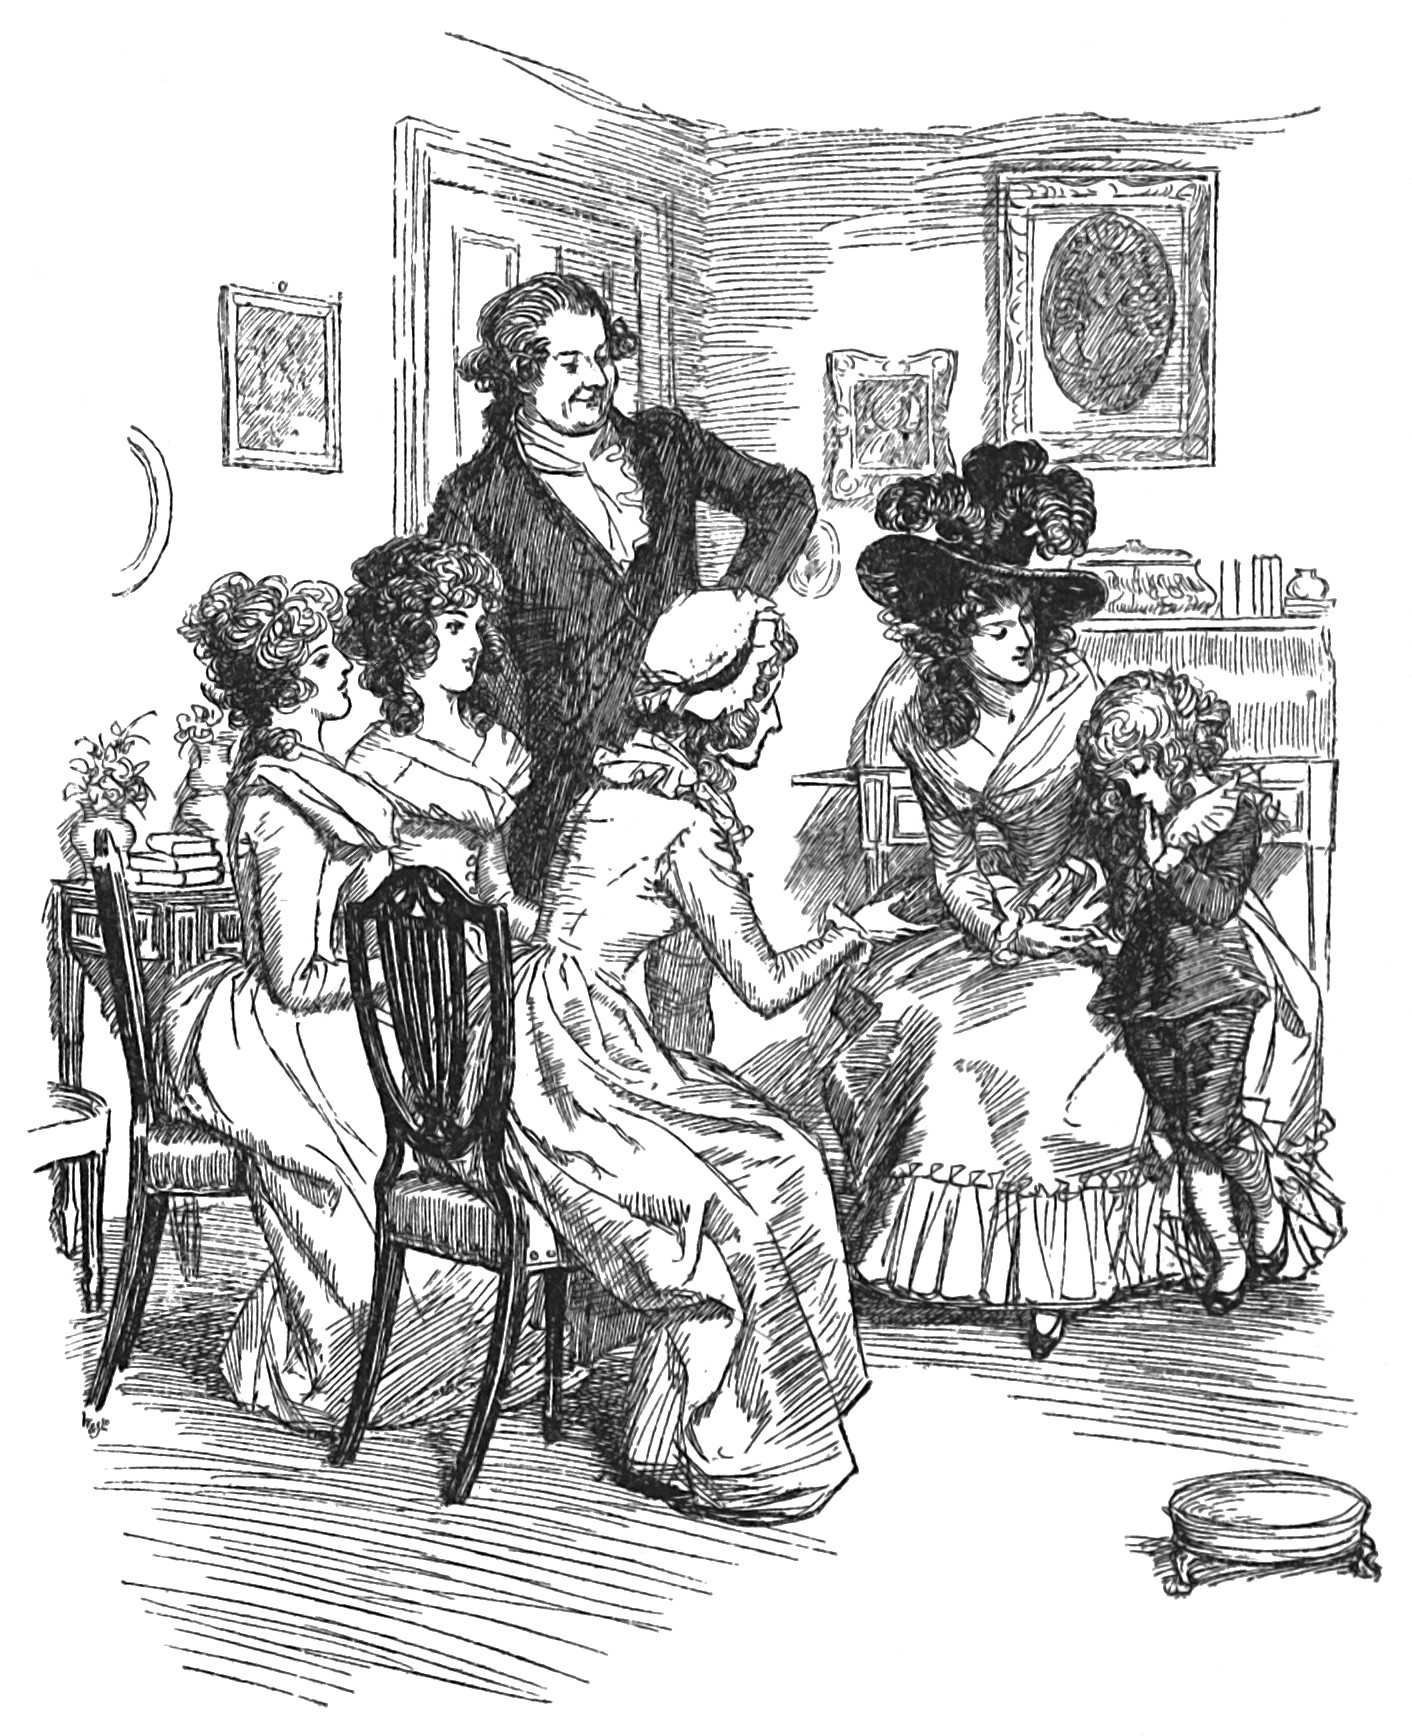
\includegraphics[width=\linewidth]{6shy}
% \caption{So shy before company}
% \end{figure}

\begin{bwbigpic}
	[1.0]
	{6shy} 
	{So shy before company} 
\end{bwbigpic}

Lady Middleton had sent a very civil message by him, denoting her intention of waiting on Mrs Dashwood as soon as she could be assured that her visit would be no inconvenience; and as this message was answered by an invitation equally polite, her ladyship was introduced to them the next day.

They were, of course, very anxious to see a person on whom so much of their comfort at Barton must depend; and the elegance of her appearance was favourable to their wishes. Lady Middleton was not more than six or seven and twenty; her face was handsome, her figure tall and striking, and her address graceful. Her manners had all the elegance which her husband's wanted. But they would have been improved by some share of his frankness and warmth; and her visit was long enough to detract something from their first admiration, by showing that, though perfectly well-bred, she was reserved, cold, and had nothing to say for herself beyond the most common-place inquiry or remark.

Conversation however was not wanted, for Sir John was very chatty, and Lady Middleton had taken the wise precaution of bringing with her their eldest child, a fine little boy about six years old, by which means there was one subject always to be recurred to by the ladies in case of extremity, for they had to enquire his name and age, admire his beauty, and ask him questions which his mother answered for him, while he hung about her and held down his head, to the great surprise of her ladyship, who wondered at his being so shy before company, as he could make noise enough at home. On every formal visit a child ought to be of the party, by way of provision for discourse. In the present case it took up ten minutes to determine whether the boy were most like his father or mother, and in what particular he resembled either, for of course every body differed, and every body was astonished at the opinion of the others.

An opportunity was soon to be given to the Dashwoods of debating on the rest of the children, as Sir John would not leave the house without securing their promise of dining at the park the next day.
\chapter{Lady~Susan Vernon to Mrs~Johnson}
  
  \begin{mail}{Churchhill.}{My dear Alicia,}
You are very good in taking notice of Frederica, and I am grateful for it as a mark of your friendship; but as I cannot have any doubt of the warmth of your affection, I am far from exacting so heavy a sacrifice. She is a stupid girl, and has nothing to recommend her. I would not, therefore, on my account, have you encumber one moment of your precious time by sending for her to Edward Street, especially as every visit is so much deducted from the grand affair of education, which I really wish to have attended to while she remains at Miss~Summers's. I want her to play and sing with some portion of taste and a good deal of assurance, as she has my hand and arm and a tolerable voice. I was so much indulged in my infant years that I was never obliged to attend to anything, and consequently am without the accomplishments which are now necessary to finish a pretty woman. Not that I am an advocate for the prevailing fashion of acquiring a perfect knowledge of all languages, arts, and sciences. It is throwing time away to be mistress of French, Italian, and German: music, singing, and drawing, \&c., will gain a woman some applause, but will not add one lover to her list—grace and manner, after all, are of the greatest importance. I do not mean, therefore, that Frederica's acquirements should be more than superficial, and I flatter myself that she will not remain long enough at school to understand anything thoroughly. I hope to see her the wife of Sir~James within a twelvemonth. You know on what I ground my hope, and it is certainly a good foundation, for school must be very humiliating to a girl of Frederica's age. And, by-the-by, you had better not invite her any more on that account, as I wish her to find her situation as unpleasant as possible. I am sure of Sir~James at any time, and could make him renew his application by a line. I shall trouble you meanwhile to prevent his forming any other attachment when he comes to town. Ask him to your house occasionally, and talk to him of Frederica, that he may not forget her. Upon the whole, I commend my own conduct in this affair extremely, and regard it as a very happy instance of circumspection and tenderness. Some mothers would have insisted on their daughter's accepting so good an offer on the first overture; but I could not reconcile it to myself to force Frederica into a marriage from which her heart revolted, and instead of adopting so harsh a measure merely propose to make it her own choice, by rendering her thoroughly uncomfortable till she does accept him—but enough of this tiresome girl. You may well wonder how I contrive to pass my time here, and for the first week it was insufferably dull. Now, however, we begin to mend, our party is enlarged by Mrs~Vernon's brother, a handsome young man, who promises me some amusement. There is something about him which rather interests me, a sort of sauciness and familiarity which I shall teach him to correct. He is lively, and seems clever, and when I have inspired him with greater respect for me than his sister's kind offices have implanted, he may be an agreeable flirt. There is exquisite pleasure in subduing an insolent spirit, in making a person predetermined to dislike acknowledge one's superiority. I have disconcerted him already by my calm reserve, and it shall be my endeavour to humble the pride of these self important De Courcys still lower, to convince Mrs~Vernon that her sisterly cautions have been bestowed in vain, and to persuade Reginald that she has scandalously belied me. This project will serve at least to amuse me, and prevent my feeling so acutely this dreadful separation from you and all whom I love.

\closeletter[Yours ever,]{S. Vernon.} 
\end{mail}
%!TeX root=../sensetop.tex
\chapter[Chapter \thechapter]{}
\lettrine[lraise=0.3]{M}{rs} Jennings was a widow with an ample jointure. She had only two daughters, both of whom she had lived to see respectably married, and she had now therefore nothing to do but to marry all the rest of the world. In the promotion of this object she was zealously active, as far as her ability reached; and missed no opportunity of projecting weddings among all the young people of her acquaintance. She was remarkably quick in the discovery of attachments, and had enjoyed the advantage of raising the blushes and the vanity of many a young lady by insinuations of her power over such a young man; and this kind of discernment enabled her soon after her arrival at Barton decisively to pronounce that Colonel Brandon was very much in love with Marianne Dashwood. She rather suspected it to be so, on the very first evening of their being together, from his listening so attentively while she sang to them; and when the visit was returned by the Middletons' dining at the cottage, the fact was ascertained by his listening to her again. It must be so. She was perfectly convinced of it. It would be an excellent match, for \textit{he} was rich, and \textit{she} was handsome. Mrs Jennings had been anxious to see Colonel Brandon well married, ever since her connection with Sir John first brought him to her knowledge; and she was always anxious to get a good husband for every pretty girl.

The immediate advantage to herself was by no means inconsiderable, for it supplied her with endless jokes against them both. At the park she laughed at the colonel, and in the cottage at Marianne. To the former her raillery was probably, as far as it regarded only himself, perfectly indifferent; but to the latter it was at first incomprehensible; and when its object was understood, she hardly knew whether most to laugh at its absurdity, or censure its impertinence, for she considered it as an unfeeling reflection on the colonel's advanced years, and on his forlorn condition as an old bachelor.

Mrs Dashwood, who could not think a man five years younger than herself, so exceedingly ancient as he appeared to the youthful fancy of her daughter, ventured to clear Mrs Jennings from the probability of wishing to throw ridicule on his age.

<But at least, Mama, you cannot deny the absurdity of the accusation, though you may not think it intentionally ill-natured. Colonel Brandon is certainly younger than Mrs Jennings, but he is old enough to be \textit{my} father; and if he were ever animated enough to be in love, must have long outlived every sensation of the kind. It is too ridiculous! When is a man to be safe from such wit, if age and infirmity will not protect him?>

<Infirmity!> said Elinor, <do you call Colonel Brandon infirm? I can easily suppose that his age may appear much greater to you than to my mother; but you can hardly deceive yourself as to his having the use of his limbs!>

<Did not you hear him complain of the rheumatism? and is not that the commonest infirmity of declining life?>

<My dearest child,> said her mother, laughing, <at this rate you must be in continual terror of \textit{my} decay; and it must seem to you a miracle that my life has been extended to the advanced age of forty.>

<Mama, you are not doing me justice. I know very well that Colonel Brandon is not old enough to make his friends yet apprehensive of losing him in the course of nature. He may live twenty years longer. But thirty-five has nothing to do with matrimony.>

<Perhaps,> said Elinor, <thirty-five and seventeen had better not have any thing to do with matrimony together. But if there should by any chance happen to be a woman who is single at seven and twenty, I should not think Colonel Brandon's being thirty-five any objection to his marrying \textit{her}.>

<A woman of seven and twenty,> said Marianne, after pausing a moment, <can never hope to feel or inspire affection again, and if her home be uncomfortable, or her fortune small, I can suppose that she might bring herself to submit to the offices of a nurse, for the sake of the provision and security of a wife. In his marrying such a woman therefore there would be nothing unsuitable. It would be a compact of convenience, and the world would be satisfied. In my eyes it would be no marriage at all, but that would be nothing. To me it would seem only a commercial exchange, in which each wished to be benefited at the expense of the other.>

<It would be impossible, I know,> replied Elinor, <to convince you that a woman of seven and twenty could feel for a man of thirty-five anything near enough to love, to make him a desirable companion to her. But I must object to your dooming Colonel Brandon and his wife to the constant confinement of a sick chamber, merely because he chanced to complain yesterday (a very cold damp day) of a slight rheumatic feel in one of his shoulders.>

<But he talked of flannel waistcoats,> said Marianne; <and with me a flannel waistcoat is invariably connected with aches, cramps, rheumatisms, and every species of ailment that can afflict the old and the feeble.>

<Had he been only in a violent fever, you would not have despised him half so much. Confess, Marianne, is not there something interesting to you in the flushed cheek, hollow eye, and quick pulse of a fever?>

Soon after this, upon Elinor's leaving the room, <Mama,> said Marianne, <I have an alarm on the subject of illness which I cannot conceal from you. I am sure Edward Ferrars is not well. We have now been here almost a fortnight, and yet he does not come. Nothing but real indisposition could occasion this extraordinary delay. What else can detain him at Norland?>

<Had you any idea of his coming so soon?> said Mrs Dashwood. <\textit{I} had none. On the contrary, if I have felt any anxiety at all on the subject, it has been in recollecting that he sometimes showed a want of pleasure and readiness in accepting my invitation, when I talked of his coming to Barton. Does Elinor expect him already?>

<I have never mentioned it to her, but of course she must.>

<I rather think you are mistaken, for when I was talking to her yesterday of getting a new grate for the spare bedchamber, she observed that there was no immediate hurry for it, as it was not likely that the room would be wanted for some time.>

<How strange this is! what can be the meaning of it! But the whole of their behaviour to each other has been unaccountable! How cold, how composed were their last adieus! How languid their conversation the last evening of their being together! In Edward's farewell there was no distinction between Elinor and me: it was the good wishes of an affectionate brother to both. Twice did I leave them purposely together in the course of the last morning, and each time did he most unaccountably follow me out of the room. And Elinor, in quitting Norland and Edward, cried not as I did. Even now her self-command is invariable. When is she dejected or melancholy? When does she try to avoid society, or appear restless and dissatisfied in it?>
%!TeX root=../pridetop.tex

\chapter[Chapter \thechapter]{}
	
	\begin{figure}[t!]
\centering
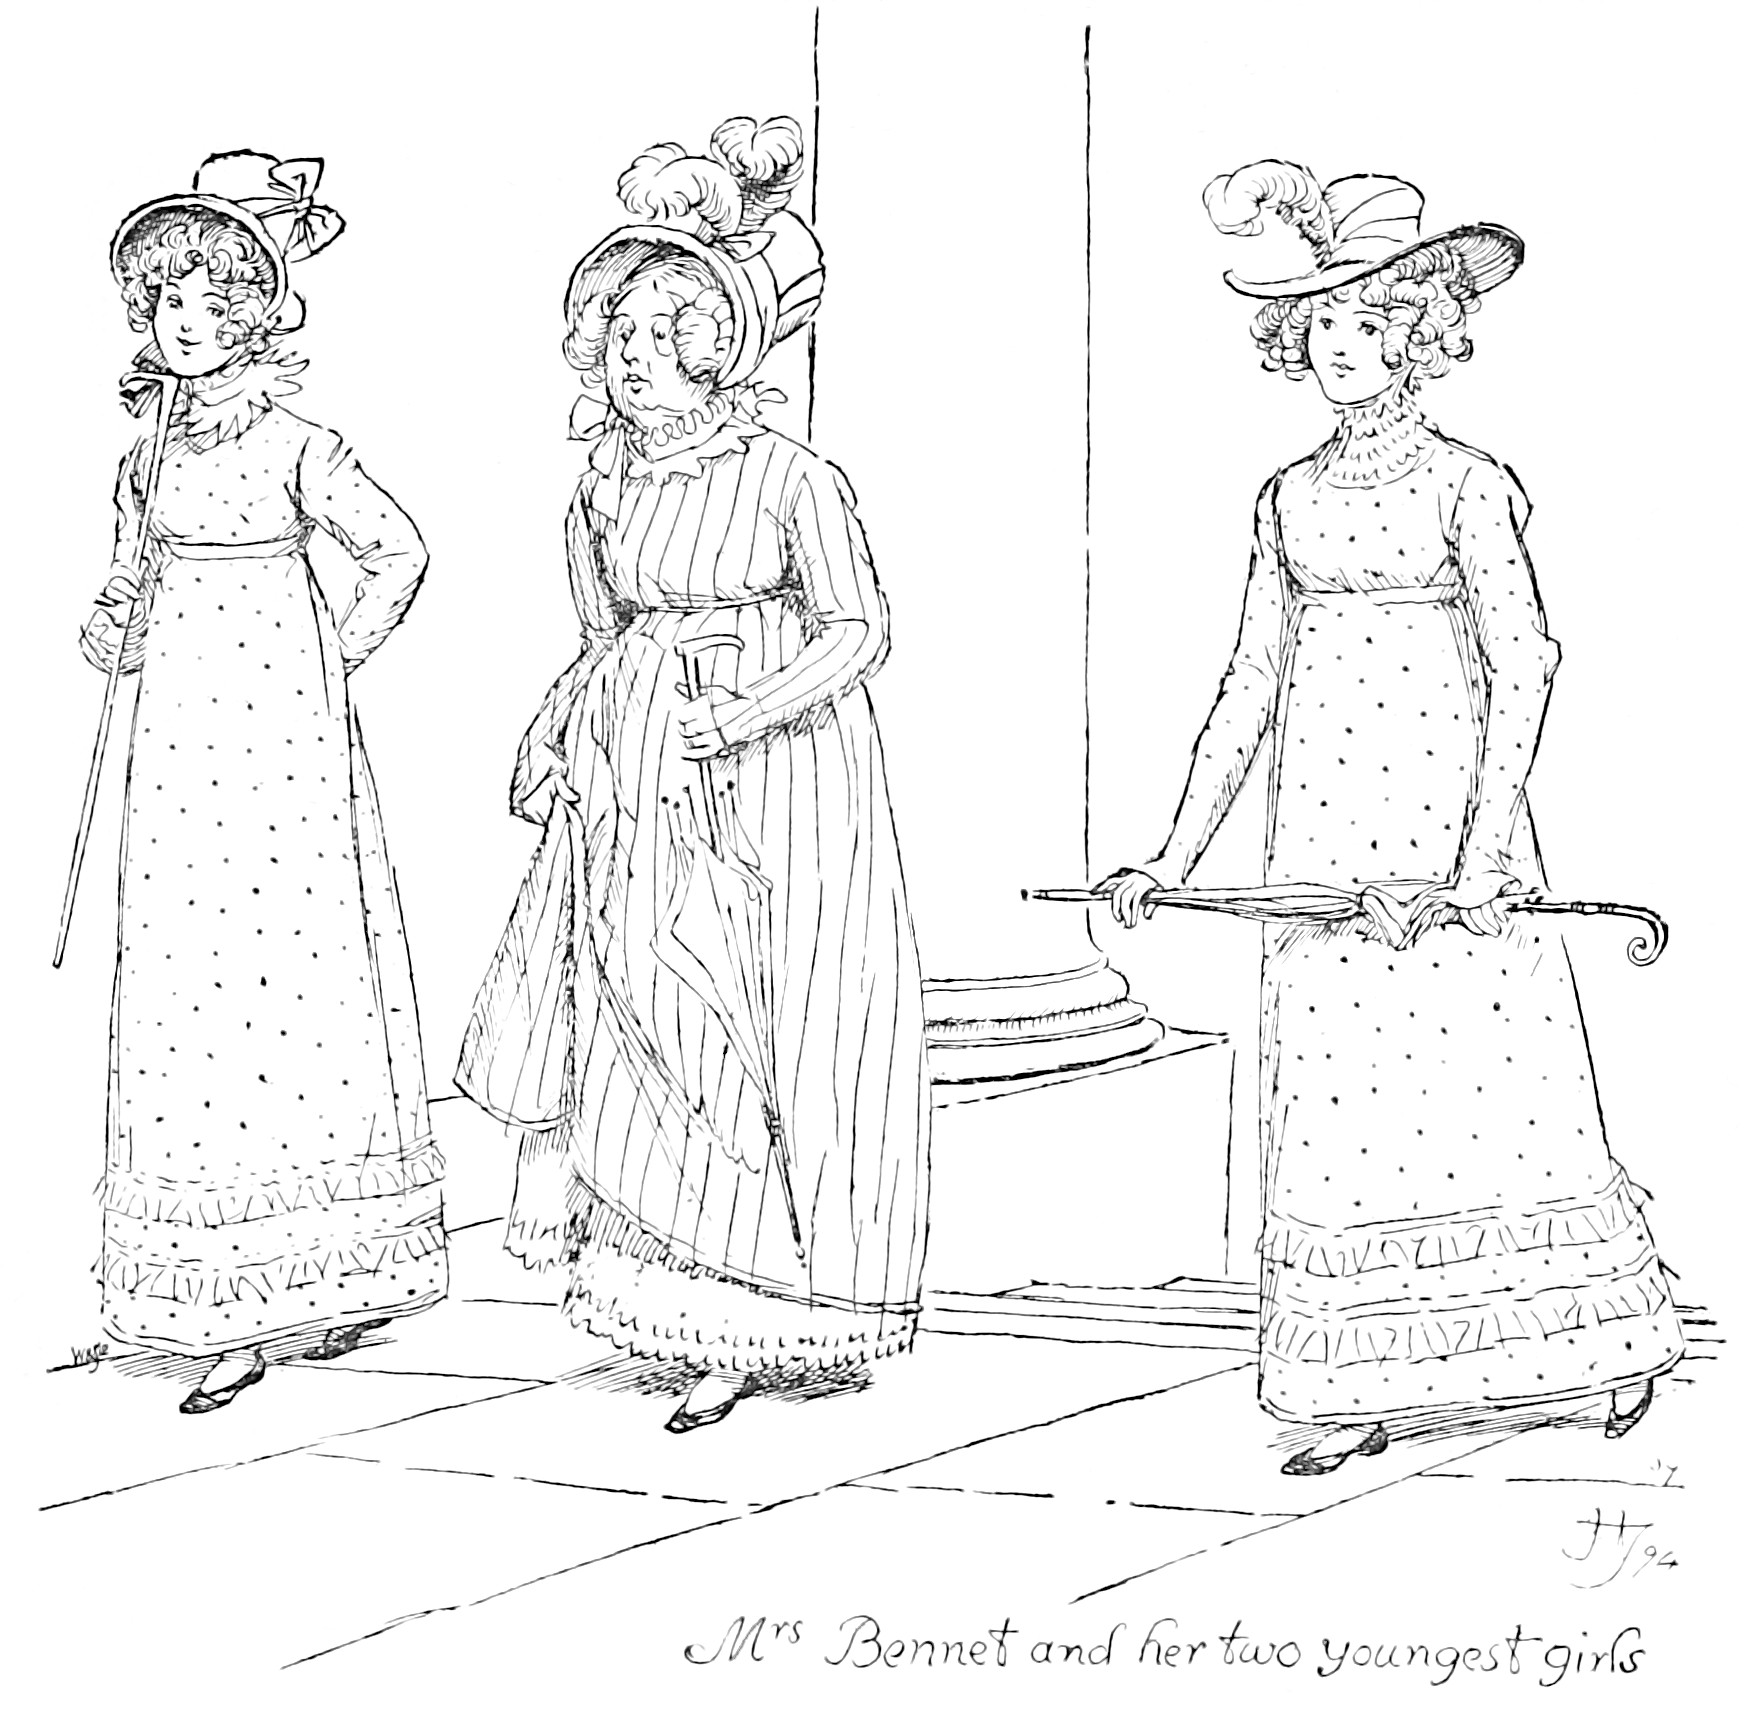
\includegraphics[width=.8\linewidth]{9bennetgirls}
\captionlistentry{Mrs Bennet and her two youngest girls}
\end{figure}

	\lettrine[lines=6,image=true]{initials/chap9e}{lizabeth}  passed the chief of the night in her sister's room, and in the morning had the pleasure of being able to send a tolerable answer to the inquiries which she very early received from Mr Bingley by a housemaid, and some time afterwards from the two elegant ladies who waited on his sisters. In spite of this amendment, however, she requested to have a note sent to Longbourn, desiring her mother to visit Jane, and form her own judgment of her situation. The note was immediately despatched, and its contents as quickly complied with. Mrs Bennet, accompanied by her two youngest girls, reached Netherfield soon after the family breakfast.



Had she found Jane in any apparent danger, Mrs Bennet would have been very miserable; but being satisfied on seeing her that her illness was not alarming, she had no wish of her recovering immediately, as her restoration to health would probably remove her from Netherfield. She would not listen, therefore, to her daughter's proposal of being carried home; neither did the apothecary, who arrived about the same time, think it at all advisable. After sitting a little while with Jane, on Miss Bingley's appearance and invitation, the mother and three daughters all attended her into the breakfast parlour. Bingley met them with hopes that Mrs Bennet had not found Miss Bennet worse than she expected.

»Indeed I have, sir,« was her answer. »She is a great deal too ill to be moved. Mr Jones says we must not think of moving her. We must trespass a little longer on your kindness.«

»Removed!« cried Bingley. »It must not be thought of. My sister, I am sure, will not hear of her removal.«

»You may depend upon it, madam,« said Miss Bingley, with cold civility, »that Miss Bennet shall receive every possible attention while she remains with us.«

Mrs Bennet was profuse in her acknowledgments.

»I am sure,« she added, »if it was not for such good friends, I do not know what would become of her, for she is very ill indeed, and suffers a vast deal, though with the greatest patience in the world, which is always the way with her, for she has, without exception, the sweetest temper I ever met with. I often tell my other girls they are nothing to \textit{her}. You have a sweet room here, Mr Bingley, and a charming prospect over that gravel walk. I do not know a place in the country that is equal to Netherfield. You will not think of quitting it in a hurry, I hope, though you have but a short lease.«

»Whatever I do is done in a hurry,« replied he; »and therefore if I should resolve to quit Netherfield, I should probably be off in five minutes. At present, however, I consider myself as quite fixed here.«

»That is exactly what I should have supposed of you,« said Elizabeth.

»You begin to comprehend me, do you?« cried he, turning towards her.

»Oh yes—I understand you perfectly.«

»I wish I might take this for a compliment; but to be so easily seen through, I am afraid, is pitiful.«

»That is as it happens. It does not necessarily follow that a deep, intricate character is more or less estimable than such a one as yours.«

»Lizzy,« cried her mother, »remember where you are, and do not run on in the wild manner that you are suffered to do at home.«

»I did not know before,« continued Bingley, immediately, »that you were a studier of character. It must be an amusing study.«

»Yes; but intricate characters are the \textit{most} amusing. They have at least that advantage.«

»The country,« said Darcy, »can in general supply but few subjects for such a study. In a country neighbourhood you move in a very confined and unvarying society.«

»But people themselves alter so much, that there is something new to be observed in them for ever.«

»Yes, indeed,« cried Mrs Bennet, offended by his manner of mentioning a country neighbourhood. »I assure you there is quite as much of \textit{that} going on in the country as in town.«

Everybody was surprised; and Darcy, after looking at her for a moment, turned silently away. Mrs Bennet, who fancied she had gained a complete victory over him, continued her triumph,—

»I cannot see that London has any great advantage over the country, for my part, except the shops and public places. The country is a vast deal pleasanter, is not it, Mr Bingley?«

»When I am in the country,« he replied, »I never wish to leave it; and when I am in town, it is pretty much the same. They have each their advantages, and I can be equally happy in either.«

»Ay, that is because you have the right disposition. But that gentleman,« looking at Darcy, »seemed to think the country was nothing at all.«

»Indeed, mamma, you are mistaken,« said Elizabeth, blushing for her mother. »You quite mistook Mr Darcy. He only meant that there was not such a variety of people to be met with in the country as in town, which you must acknowledge to be true.«

»Certainly, my dear, nobody said there were; but as to not meeting with many people in this neighbourhood, I believe there are few neighbourhoods larger. I know we dine with four-and-twenty families.«

Nothing but concern for Elizabeth could enable Bingley to keep his countenance. His sister was less delicate, and directed her eye towards Mr Darcy with a very expressive smile. Elizabeth, for the sake of saying something that might turn her mother's thoughts, now asked her if Charlotte Lucas had been at Longbourn since \textit{her} coming away.

»Yes, she called yesterday with her father. What an agreeable man Sir William is, Mr Bingley—is not he? so much the man of fashion! so genteel and so easy! He has always something to say to everybody. \textit{That} is my idea of good breeding; and those persons who fancy themselves very important and never open their mouths quite mistake the matter.«

»Did Charlotte dine with you?«

»No, she would go home. I fancy she was wanted about the mince-pies. For my part, Mr Bingley, \textit{I} always keep servants that can do their own work; \textit{my} daughters are brought up differently. But everybody is to judge for themselves, and the Lucases are a very good sort of girls, I assure you. It is a pity they are not handsome! Not that \textit{I} think Charlotte so \textit{very} plain; but then she is our particular friend.«

»She seems a very pleasant young woman,« said Bingley.

»Oh dear, yes; but you must own she is very plain. Lady Lucas herself has often said so, and envied me Jane's beauty. I do not like to boast of my own child; but to be sure, Jane—one does not often see anybody better looking. It is what everybody says. I do not trust my own partiality. When she was only fifteen there was a gentleman at my brother Gardiner's in town so much in love with her, that my sister-in-law was sure he would make her an offer before we came away. But, however, he did not. Perhaps he thought her too young. However, he wrote some verses on her, and very pretty they were.«

»And so ended his affection,« said Elizabeth, impatiently. »There has been many a one, I fancy, overcome in the same way. I wonder who first discovered the efficacy of poetry in driving away love!«

»I have been used to consider poetry as the \textit{food} of love,« said Darcy.

»Of a fine, stout, healthy love it may. Everything nourishes what is strong already. But if it be only a slight, thin sort of inclination, I am convinced that one good sonnet will starve it entirely away.«

Darcy only smiled; and the general pause which ensued made Elizabeth tremble lest her mother should be exposing herself again. She longed to speak, but could think of nothing to say; and after a short silence Mrs Bennet began repeating her thanks to Mr Bingley for his kindness to Jane, with an apology for troubling him also with Lizzy. Mr Bingley was unaffectedly civil in his answer, and forced his younger sister to be civil also, and say what the occasion required. She performed her part, indeed, without much graciousness, but Mrs Bennet was satisfied, and soon afterwards ordered her carriage. Upon this signal, the youngest of her daughters put herself forward. The two girls had been whispering to each other during the whole visit; and the result of it was, that the youngest should tax Mr Bingley with having promised on his first coming into the country to give a ball at Netherfield.

Lydia was a stout, well-grown girl of fifteen, with a fine complexion and good-humoured countenance; a favourite with her mother, whose affection had brought her into public at an early age. She had high animal spirits, and a sort of natural \newline self-consequence, which the attentions of the officers, to whom her uncle's good dinners and her own easy manners recommended her, had increased into assurance. She was very equal, therefore, to address Mr Bingley on the subject of the ball, and abruptly reminded him of his promise; adding, that it would be the most shameful thing in the world if he did not keep it. His answer to this sudden attack was delightful to her mother's ear.

»I am perfectly ready, I assure you, to keep my engagement; and, when your sister is recovered, you shall, if you please, name the very day of the ball. But you would not wish to be dancing while she is ill?«

Lydia declared herself satisfied. »Oh yes—it would be much better to wait till Jane was well; and by that time, most likely, Captain Carter would be at Meryton again. And when you have given \textit{your} ball,« she added, »I shall insist on their giving one also. I shall tell Colonel Forster it will be quite a shame if he does not.«

Mrs Bennet and her daughters then departed, and Elizabeth returned instantly to Jane, leaving her own and her relations' behaviour to the remarks of the two ladies and Mr Darcy; the latter of whom, however, could not be prevailed on to join in their censure of \textit{her}, in spite of all Miss Bingley's witticisms on \textit{fine eyes}.
%!TeX root=../emmatop.tex
\chapter[Chapter \thechapter]{}
\lettrine[lraise=0.3]{T}{hough} now the middle of December, there had yet been no weather to prevent the young ladies from tolerably regular exercise; and on the morrow, Emma had a charitable visit to pay to a poor sick family, who lived a little way out of Highbury.

Their road to this detached cottage was down Vicarage Lane, a lane leading at right angles from the broad, though irregular, main street of the place; and, as may be inferred, containing the blessed abode of Mr Elton. A few inferior dwellings were first to be passed, and then, about a quarter of a mile down the lane rose the Vicarage, an old and not very good house, almost as close to the road as it could be. It had no advantage of situation; but had been very much smartened up by the present proprietor; and, such as it was, there could be no possibility of the two friends passing it without a slackened pace and observing eyes.—Emma's remark was—

<There it is. There go you and your riddle-book one of these days.>—Harriet's was—

<Oh, what a sweet house!—How very beautiful!—There are the yellow curtains that Miss Nash admires so much.>

<I do not often walk this way \textit{now},> said Emma, as they proceeded, <but \textit{then} there will be an inducement, and I shall gradually get intimately acquainted with all the hedges, gates, pools and pollards of this part of Highbury.>

Harriet, she found, had never in her life been inside the Vicarage, and her curiosity to see it was so extreme, that, considering exteriors and probabilities, Emma could only class it, as a proof of love, with Mr Elton's seeing ready wit in her.

<I wish we could contrive it,> said she; <but I cannot think of any tolerable pretence for going in;—no servant that I want to inquire about of his housekeeper—no message from my father.>

She pondered, but could think of nothing. After a mutual silence of some minutes, Harriet thus began again—

<I do so wonder, Miss Woodhouse, that you should not be married, or going to be married! so charming as you are!>—

Emma laughed, and replied,

<My being charming, Harriet, is not quite enough to induce me to marry; I must find other people charming—one other person at least. And I am not only, not going to be married, at present, but have very little intention of ever marrying at all.>

<Ah!—so you say; but I cannot believe it.>

<I must see somebody very superior to any one I have seen yet, to be tempted; Mr Elton, you know, (recollecting herself,) is out of the question: and I do \textit{not} wish to see any such person. I would rather not be tempted. I cannot really change for the better. If I were to marry, I must expect to repent it.>

<Dear me!—it is so odd to hear a woman talk so!>—

<I have none of the usual inducements of women to marry. Were I to fall in love, indeed, it would be a different thing! but I never have been in love; it is not my way, or my nature; and I do not think I ever shall. And, without love, I am sure I should be a fool to change such a situation as mine. Fortune I do not want; employment I do not want; consequence I do not want: I believe few married women are half as much mistress of their husband's house as I am of Hartfield; and never, never could I expect to be so truly beloved and important; so always first and always right in any man's eyes as I am in my father's.>

<But then, to be an old maid at last, like Miss Bates!>

<That is as formidable an image as you could present, Harriet; and if I thought I should ever be like Miss Bates! so silly—so satisfied—so smiling—so prosing—so undistinguishing and unfastidious—and so apt to tell every thing relative to every body about me, I would marry to-morrow. But between \textit{us}, I am convinced there never can be any likeness, except in being unmarried.>

<But still, you will be an old maid! and that's so dreadful!>

<Never mind, Harriet, I shall not be a poor old maid; and it is poverty only which makes celibacy contemptible to a generous public! A single woman, with a very narrow income, must be a ridiculous, disagreeable old maid! the proper sport of boys and girls, but a single woman, of good fortune, is always respectable, and may be as sensible and pleasant as any body else. And the distinction is not quite so much against the candour and common sense of the world as appears at first; for a very narrow income has a tendency to contract the mind, and sour the temper. Those who can barely live, and who live perforce in a very small, and generally very inferior, society, may well be illiberal and cross. This does not apply, however, to Miss Bates; she is only too good natured and too silly to suit me; but, in general, she is very much to the taste of every body, though single and though poor. Poverty certainly has not contracted her mind: I really believe, if she had only a shilling in the world, she would be very likely to give away sixpence of it; and nobody is afraid of her: that is a great charm.>

<Dear me! but what shall you do? how shall you employ yourself when you grow old?>

<If I know myself, Harriet, mine is an active, busy mind, with a great many independent resources; and I do not perceive why I should be more in want of employment at forty or fifty than one-and-twenty. Woman's usual occupations of hand and mind will be as open to me then as they are now; or with no important variation. If I draw less, I shall read more; if I give up music, I shall take to carpet-work. And as for objects of interest, objects for the affections, which is in truth the great point of inferiority, the want of which is really the great evil to be avoided in \textit{not} marrying, I shall be very well off, with all the children of a sister I love so much, to care about. There will be enough of them, in all probability, to supply every sort of sensation that declining life can need. There will be enough for every hope and every fear; and though my attachment to none can equal that of a parent, it suits my ideas of comfort better than what is warmer and blinder. My nephews and nieces!—I shall often have a niece with me.>

<Do you know Miss Bates's niece? That is, I know you must have seen her a hundred times—but are you acquainted?>

<Oh! yes; we are always forced to be acquainted whenever she comes to Highbury. By the bye, \textit{that} is almost enough to put one out of conceit with a niece. Heaven forbid! at least, that I should ever bore people half so much about all the Knightleys together, as she does about Jane Fairfax. One is sick of the very name of Jane Fairfax. Every letter from her is read forty times over; her compliments to all friends go round and round again; and if she does but send her aunt the pattern of a stomacher, or knit a pair of garters for her grandmother, one hears of nothing else for a month. I wish Jane Fairfax very well; but she tires me to death.>

They were now approaching the cottage, and all idle topics were superseded. Emma was very compassionate; and the distresses of the poor were as sure of relief from her personal attention and kindness, her counsel and her patience, as from her purse. She understood their ways, could allow for their ignorance and their temptations, had no romantic expectations of extraordinary virtue from those for whom education had done so little; entered into their troubles with ready sympathy, and always gave her assistance with as much intelligence as good-will. In the present instance, it was sickness and poverty together which she came to visit; and after remaining there as long as she could give comfort or advice, she quitted the cottage with such an impression of the scene as made her say to Harriet, as they walked away,

<These are the sights, Harriet, to do one good. How trifling they make every thing else appear!—I feel now as if I could think of nothing but these poor creatures all the rest of the day; and yet, who can say how soon it may all vanish from my mind?>

<Very true,> said Harriet. <Poor creatures! one can think of nothing else.>

<And really, I do not think the impression will soon be over,> said Emma, as she crossed the low hedge, and tottering footstep which ended the narrow, slippery path through the cottage garden, and brought them into the lane again. <I do not think it will,> stopping to look once more at all the outward wretchedness of the place, and recall the still greater within.

<Oh! dear, no,> said her companion.

They walked on. The lane made a slight bend; and when that bend was passed, Mr Elton was immediately in sight; and so near as to give Emma time only to say farther,

<Ah! Harriet, here comes a very sudden trial of our stability in good thoughts. Well, (smiling,) I hope it may be allowed that if compassion has produced exertion and relief to the sufferers, it has done all that is truly important. If we feel for the wretched, enough to do all we can for them, the rest is empty sympathy, only distressing to ourselves.>

Harriet could just answer, <Oh! dear, yes,> before the gentleman joined them. The wants and sufferings of the poor family, however, were the first subject on meeting. He had been going to call on them. His visit he would now defer; but they had a very interesting parley about what could be done and should be done. Mr Elton then turned back to accompany them.

<To fall in with each other on such an errand as this,> thought Emma; <to meet in a charitable scheme; this will bring a great increase of love on each side. I should not wonder if it were to bring on the declaration. It must, if I were not here. I wish I were anywhere else.>

Anxious to separate herself from them as far as she could, she soon afterwards took possession of a narrow footpath, a little raised on one side of the lane, leaving them together in the main road. But she had not been there two minutes when she found that Harriet's habits of dependence and imitation were bringing her up too, and that, in short, they would both be soon after her. This would not do; she immediately stopped, under pretence of having some alteration to make in the lacing of her half-boot, and stooping down in complete occupation of the footpath, begged them to have the goodness to walk on, and she would follow in half a minute. They did as they were desired; and by the time she judged it reasonable to have done with her boot, she had the comfort of farther delay in her power, being overtaken by a child from the cottage, setting out, according to orders, with her pitcher, to fetch broth from Hartfield. To walk by the side of this child, and talk to and question her, was the most natural thing in the world, or would have been the most natural, had she been acting just then without design; and by this means the others were still able to keep ahead, without any obligation of waiting for her. She gained on them, however, involuntarily: the child's pace was quick, and theirs rather slow; and she was the more concerned at it, from their being evidently in a conversation which interested them. Mr Elton was speaking with animation, Harriet listening with a very pleased attention; and Emma, having sent the child on, was beginning to think how she might draw back a little more, when they both looked around, and she was obliged to join them.

Mr Elton was still talking, still engaged in some interesting detail; and Emma experienced some disappointment when she found that he was only giving his fair companion an account of the yesterday's party at his friend Cole's, and that she was come in herself for the Stilton cheese, the north Wiltshire, the butter, the celery, the beet-root, and all the dessert.

<This would soon have led to something better, of course,> was her consoling reflection; <any thing interests between those who love; and any thing will serve as introduction to what is near the heart. If I could but have kept longer away!>

They now walked on together quietly, till within view of the vicarage pales, when a sudden resolution, of at least getting Harriet into the house, made her again find something very much amiss about her boot, and fall behind to arrange it once more. She then broke the lace off short, and dexterously throwing it into a ditch, was presently obliged to entreat them to stop, and acknowledged her inability to put herself to rights so as to be able to walk home in tolerable comfort.

<Part of my lace is gone,> said she, <and I do not know how I am to contrive. I really am a most troublesome companion to you both, but I hope I am not often so ill-equipped. Mr Elton, I must beg leave to stop at your house, and ask your housekeeper for a bit of ribband or string, or any thing just to keep my boot on.>

Mr Elton looked all happiness at this proposition; and nothing could exceed his alertness and attention in conducting them into his house and endeavouring to make every thing appear to advantage. The room they were taken into was the one he chiefly occupied, and looking forwards; behind it was another with which it immediately communicated; the door between them was open, and Emma passed into it with the housekeeper to receive her assistance in the most comfortable manner. She was obliged to leave the door ajar as she found it; but she fully intended that Mr Elton should close it. It was not closed, however, it still remained ajar; but by engaging the housekeeper in incessant conversation, she hoped to make it practicable for him to chuse his own subject in the adjoining room. For ten minutes she could hear nothing but herself. It could be protracted no longer. She was then obliged to be finished, and make her appearance.

The lovers were standing together at one of the windows. It had a most favourable aspect; and, for half a minute, Emma felt the glory of having schemed successfully. But it would not do; he had not come to the point. He had been most agreeable, most delightful; he had told Harriet that he had seen them go by, and had purposely followed them; other little gallantries and allusions had been dropt, but nothing serious.

<Cautious, very cautious,> thought Emma; <he advances inch by inch, and will hazard nothing till he believes himself secure.>

Still, however, though every thing had not been accomplished by her ingenious device, she could not but flatter herself that it had been the occasion of much present enjoyment to both, and must be leading them forward to the great event.
%!TeX root=../persuasiontop.tex
\chapter[Chapter \thechapter]{}

\begin{figure}[t!]
\centering

\includegraphics[width=\linewidth]{nouveau11}
\end{figure}

\lettrine[lines=4,lraise=0.3]{T}{he} time now approached for Lady Russell's return: the day was even fixed; and Anne, being engaged to join her as soon as she was resettled, was looking forward to an early removal to Kellynch, and beginning to think how her own comfort was likely to be affected by it.

It would place her in the same village with Captain Wentworth, within half a mile of him; they would have to frequent the same church, and there must be intercourse between the two families. This was against her; but on the other hand, he spent so much of his time at Uppercross, that in removing thence she might be considered rather as leaving him behind, than as going towards him; and, upon the whole, she believed she must, on this interesting question, be the gainer, almost as certainly as in her change of domestic society, in leaving poor Mary for Lady Russell.

She wished it might be possible for her to avoid ever seeing Captain Wentworth at the Hall: those rooms had witnessed former meetings which would be brought too painfully before her; but she was yet more anxious for the possibility of Lady Russell and Captain Wentworth never meeting anywhere. They did not like each other, and no renewal of acquaintance now could do any good; and were Lady Russell to see them together, she might think that he had too much self-possession, and she too little.

These points formed her chief solicitude in anticipating her removal from Uppercross, where she felt she had been stationed quite long enough. Her usefulness to little Charles would always give some sweetness to the memory of her two months' visit there, but he was gaining strength apace, and she had nothing else to stay for.

The conclusion of her visit, however, was diversified in a way which she had not at all imagined. Captain Wentworth, after being unseen and unheard of at Uppercross for two whole days, appeared again among them to justify himself by a relation of what had kept him away.

A letter from his friend, Captain Harville, having found him out at last, had brought intelligence of Captain Harville's being settled with his family at Lyme for the winter; of their being therefore, quite unknowingly, within twenty miles of each other. Captain Harville had never been in good health since a severe wound which he received two years before, and Captain Wentworth's anxiety to see him had determined him to go immediately to Lyme. He had been there for four-and-twenty hours. His acquittal was complete, his friendship warmly honoured, a lively interest excited for his friend, and his description of the fine country about Lyme so feelingly attended to by the party, that an earnest desire to see Lyme themselves, and a project for going thither was the consequence.

The young people were all wild to see Lyme. Captain Wentworth talked of going there again himself, it was only seventeen miles from Uppercross; though November, the weather was by no means bad; and, in short, Louisa, who was the most eager of the eager, having formed the resolution to go, and besides the pleasure of doing as she liked, being now armed with the idea of merit in maintaining her own way, bore down all the wishes of her father and mother for putting it off till summer; and to Lyme they were to go—Charles, Mary, Anne, Henrietta, Louisa, and Captain Wentworth.

The first heedless scheme had been to go in the morning and return at night; but to this Mr Musgrove, for the sake of his horses, would not consent; and when it came to be rationally considered, a day in the middle of November would not leave much time for seeing a new place, after deducting seven hours, as the nature of the country required, for going and returning. They were, consequently, to stay the night there, and not to be expected back till the next day's dinner. This was felt to be a considerable amendment; and though they all met at the Great House at rather an early breakfast hour, and set off very punctually, it was so much past noon before the two carriages, Mr Musgrove's coach containing the four ladies, and Charles's curricle, in which he drove Captain Wentworth, were descending the long hill into Lyme, and entering upon the still steeper street of the town itself, that it was very evident they would not have more than time for looking about them, before the light and warmth of the day were gone.

After securing accommodations, and ordering a dinner at one of the inns, the next thing to be done was unquestionably to walk directly down to the sea. They were come too late in the year for any amusement or variety which Lyme, as a public place, might offer. The rooms were shut up, the lodgers almost all gone, scarcely any family but of the residents left; and, as there is nothing to admire in the buildings themselves, the remarkable situation of the town, the principal street almost hurrying into the water, the walk to the Cobb, skirting round the pleasant little bay, which, in the season, is animated with bathing machines and company; the Cobb itself, its old wonders and new improvements, with the very beautiful line of cliffs stretching out to the east of the town, are what the stranger's eye will seek; and a very strange stranger it must be, who does not see charms in the immediate environs of Lyme, to make him wish to know it better. The scenes in its neighbourhood, Charmouth, with its high grounds and extensive sweeps of country, and still more, its sweet, retired bay, backed by dark cliffs, where fragments of low rock among the sands, make it the happiest spot for watching the flow of the tide, for sitting in unwearied contemplation; the woody varieties of the cheerful village of Up Lyme; and, above all, Pinny, with its green chasms between romantic rocks, where the scattered forest trees and orchards of luxuriant growth, declare that many a generation must have passed away since the first partial falling of the cliff prepared the ground for such a state, where a scene so wonderful and so lovely is exhibited, as may more than equal any of the resembling scenes of the far-famed Isle of Wight: these places must be visited, and visited again, to make the worth of Lyme understood.

The party from Uppercross passing down by the now deserted and melancholy looking rooms, and still descending, soon found themselves on the sea-shore; and lingering only, as all must linger and gaze on a first return to the sea, who ever deserved to look on it at all, proceeded towards the Cobb, equally their object in itself and on Captain Wentworth's account: for in a small house, near the foot of an old pier of unknown date, were the Harvilles settled. Captain Wentworth turned in to call on his friend; the others walked on, and he was to join them on the Cobb.

They were by no means tired of wondering and admiring; and not even Louisa seemed to feel that they had parted with Captain Wentworth long, when they saw him coming after them, with three companions, all well known already, by description, to be Captain and Mrs Harville, and a Captain Benwick, who was staying with them.

Captain Benwick had some time ago been first lieutenant of the Laconia; and the account which Captain Wentworth had given of him, on his return from Lyme before, his warm praise of him as an excellent young man and an officer, whom he had always valued highly, which must have stamped him well in the esteem of every listener, had been followed by a little history of his private life, which rendered him perfectly interesting in the eyes of all the ladies. He had been engaged to Captain Harville's sister, and was now mourning her loss. They had been a year or two waiting for fortune and promotion. Fortune came, his prize-money as lieutenant being great; promotion, too, came at \textit{last}; but Fanny Harville did not live to know it. She had died the preceding summer while he was at sea. Captain Wentworth believed it impossible for man to be more attached to woman than poor Benwick had been to Fanny Harville, or to be more deeply afflicted under the dreadful change. He considered his disposition as of the sort which must suffer heavily, uniting very strong feelings with quiet, serious, and retiring manners, and a decided taste for reading, and sedentary pursuits. To finish the interest of the story, the friendship between him and the Harvilles seemed, if possible, augmented by the event which closed all their views of alliance, and Captain Benwick was now living with them entirely. Captain Harville had taken his present house for half a year; his taste, and his health, and his fortune, all directing him to a residence inexpensive, and by the sea; and the grandeur of the country, and the retirement of Lyme in the winter, appeared exactly adapted to Captain Benwick's state of mind. The sympathy and good-will excited towards Captain Benwick was very great.

»And yet,« said Anne to herself, as they now moved forward to meet the party, »he has not, perhaps, a more sorrowing heart than I have. I cannot believe his prospects so blighted for ever. He is younger than I am; younger in feeling, if not in fact; younger as a man. He will rally again, and be happy with another.«

They all met, and were introduced. Captain Harville was a tall, dark man, with a sensible, benevolent countenance; a little lame; and from strong features and want of health, looking much older than Captain Wentworth. Captain Benwick looked, and was, the youngest of the three, and, compared with either of them, a little man. He had a pleasing face and a melancholy air, just as he ought to have, and drew back from conversation.

Captain Harville, though not equalling Captain Wentworth in manners, was a perfect gentleman, unaffected, warm, and obliging. Mrs Harville, a degree less polished than her husband, seemed, however, to have the same good feelings; and nothing could be more pleasant than their desire of considering the whole party as friends of their own, because the friends of Captain Wentworth, or more kindly hospitable than their entreaties for their all promising to dine with them. The dinner, already ordered at the inn, was at last, though unwillingly, accepted as a excuse; but they seemed almost hurt that Captain Wentworth should have brought any such party to Lyme, without considering it as a thing of course that they should dine with them.

There was so much attachment to Captain Wentworth in all this, and such a bewitching charm in a degree of hospitality so uncommon, so unlike the usual style of give-and-take invitations, and dinners of formality and display, that Anne felt her spirits not likely to be benefited by an increasing acquaintance among his brother-officers. »These would have been all my friends,« was her thought; and she had to struggle against a great tendency to lowness.

On quitting the Cobb, they all went in-doors with their new friends, and found rooms so small as none but those who invite from the heart could think capable of accommodating so many. Anne had a moment's astonishment on the subject herself; but it was soon lost in the pleasanter feelings which sprang from the sight of all the ingenious contrivances and nice arrangements of Captain Harville, to turn the actual space to the best account, to supply the deficiencies of lodging-house furniture, and defend the windows and doors against the winter storms to be expected. The varieties in the fitting-up of the rooms, where the common necessaries provided by the owner, in the common indifferent plight, were contrasted with some few articles of a rare species of wood, excellently worked up, and with something curious and valuable from all the distant countries Captain Harville had visited, were more than amusing to Anne; connected as it all was with his profession, the fruit of its labours, the effect of its influence on his habits, the picture of repose and domestic happiness it presented, made it to her a something more, or less, than gratification.

Captain Harville was no reader; but he had contrived excellent accommodations, and fashioned very pretty shelves, for a tolerable collection of well-bound volumes, the property of Captain Benwick. His lameness prevented him from taking much exercise; but a mind of usefulness and ingenuity seemed to furnish him with constant employment within. He drew, he varnished, he carpentered, he glued; he made toys for the children; he fashioned new netting-needles and pins with improvements; and if everything else was done, sat down to his large fishing-net at one corner of the room.

Anne thought she left great happiness behind her when they quitted the house; and Louisa, by whom she found herself walking, burst forth into raptures of admiration and delight on the character of the navy; their friendliness, their brotherliness, their openness, their uprightness; protesting that she was convinced of sailors having more worth and warmth than any other set of men in England; that they only knew how to live, and they only deserved to be respected and loved.

They went back to dress and dine; and so well had the scheme answered already, that nothing was found amiss; though its being »so entirely out of season,« and the »no thoroughfare of Lyme,« and the »no expectation of company,« had brought many apologies from the heads of the inn.

Anne found herself by this time growing so much more hardened to being in Captain Wentworth's company than she had at first imagined could ever be, that the sitting down to the same table with him now, and the interchange of the common civilities attending on it (they never got beyond), was become a mere nothing.

The nights were too dark for the ladies to meet again till the morrow, but Captain Harville had promised them a visit in the evening; and he came, bringing his friend also, which was more than had been expected, it having been agreed that Captain Benwick had all the appearance of being oppressed by the presence of so many strangers. He ventured among them again, however, though his spirits certainly did not seem fit for the mirth of the party in general.

While Captains Wentworth and Harville led the talk on one side of the room, and by recurring to former days, supplied anecdotes in abundance to occupy and entertain the others, it fell to Anne's lot to be placed rather apart with Captain Benwick; and a very good impulse of her nature obliged her to begin an acquaintance with him. He was shy, and disposed to abstraction; but the engaging mildness of her countenance, and gentleness of her manners, soon had their effect; and Anne was well repaid the first trouble of exertion. He was evidently a young man of considerable taste in reading, though principally in poetry; and besides the persuasion of having given him at least an evening's indulgence in the discussion of subjects, which his usual companions had probably no concern in, she had the hope of being of real use to him in some suggestions as to the duty and benefit of struggling against affliction, which had naturally grown out of their conversation. For, though shy, he did not seem reserved; it had rather the appearance of feelings glad to burst their usual restraints; and having talked of poetry, the richness of the present age, and gone through a brief comparison of opinion as to the first-rate poets, trying to ascertain whether \textit{Marmion} or \textit{The Lady of the Lake} were to be preferred, and how ranked the \textit{Giaour} and \textit{The Bride of Abydos}; and moreover, how the \textit{Giaour} was to be pronounced, he showed himself so intimately acquainted with all the tenderest songs of the one poet, and all the impassioned descriptions of hopeless agony of the other; he repeated, with such tremulous feeling, the various lines which imaged a broken heart, or a mind destroyed by wretchedness, and looked so entirely as if he meant to be understood, that she ventured to hope he did not always read only poetry, and to say, that she thought it was the misfortune of poetry to be seldom safely enjoyed by those who enjoyed it completely; and that the strong feelings which alone could estimate it truly were the very feelings which ought to taste it but sparingly.

His looks shewing him not pained, but pleased with this allusion to his situation, she was emboldened to go on; and feeling in herself the right of seniority of mind, she ventured to recommend a larger allowance of prose in his daily study; and on being requested to particularize, mentioned such works of our best moralists, such collections of the finest letters, such memoirs of characters of worth and suffering, as occurred to her at the moment as calculated to rouse and fortify the mind by the highest precepts, and the strongest examples of moral and religious endurances.

Captain Benwick listened attentively, and seemed grateful for the interest implied; and though with a shake of the head, and sighs which declared his little faith in the efficacy of any books on grief like his, noted down the names of those she recommended, and promised to procure and read them.

When the evening was over, Anne could not but be amused at the idea of her coming to Lyme to preach patience and resignation to a young man whom she had never seen before; nor could she help fearing, on more serious reflection, that, like many other great moralists and preachers, she had been eloquent on a point in which her own conduct would ill bear examination.
\chapter{Sir~Reginald De Courcy to his Son}
  
  \begin{mail}{Parklands.}{}

I know that young men in general do not admit of any enquiry even from their nearest relations into affairs of the heart, but I hope, my dear Reginald, that you will be superior to such as allow nothing for a father's anxiety, and think themselves privileged to refuse him their confidence and slight his advice. You must be sensible that as an only son, and the representative of an ancient family, your conduct in life is most interesting to your connections; and in the very important concern of marriage especially, there is everything at stake—your own happiness, that of your parents, and the credit of your name. I do not suppose that you would deliberately form an absolute engagement of that nature without acquainting your mother and myself, or at least, without being convinced that we should approve of your choice; but I cannot help fearing that you may be drawn in, by the Lady~who has lately attached you, to a marriage which the whole of your family, far and near, must highly reprobate. Lady~Susan's age is itself a material objection, but her want of character is one so much more serious, that the difference of even twelve years becomes in comparison of small amount. Were you not blinded by a sort of fascination, it would be ridiculous in me to repeat the instances of great misconduct on her side so very generally known.

Her neglect of her husband, her encouragement of other men, her extravagance and dissipation, were so gross and notorious that no one could be ignorant of them at the time, nor can now have forgotten them. To our family she has always been represented in softened colours by the benevolence of Mr~Charles Vernon, and yet, in spite of his generous endeavours to excuse her, we know that she did, from the most selfish motives, take all possible pains to prevent his marriage with Catherine.

My years and increasing infirmities make me very desirous of seeing you settled in the world. To the fortune of a wife, the goodness of my own will make me indifferent, but her family and character must be equally unexceptionable. When your choice is fixed so that no objection can be made to it, then I can promise you a ready and cheerful consent; but it is my duty to oppose a match which deep art only could render possible, and must in the end make wretched. It is possible her behaviour may arise only from vanity, or the wish of gaining the admiration of a man whom she must imagine to be particularly prejudiced against her; but it is more likely that she should aim at something further. She is poor, and may naturally seek an alliance which must be advantageous to herself; you know your own rights, and that it is out of my power to prevent your inheriting the family estate. My ability of distressing you during my life would be a species of revenge to which I could hardly stoop under any circumstances.

I honestly tell you my sentiments and intentions: I do not wish to work on your fears, but on your sense and affection. It would destroy every comfort of my life to know that you were married to Lady~Susan Vernon; it would be the death of that honest pride with which I have hitherto considered my son; I should blush to see him, to hear of him, to think of him. I may perhaps do no good but that of relieving my own mind by this letter, but I felt it my duty to tell you that your partiality for Lady~Susan is no secret to your friends, and to warn you against her. I should be glad to hear your reasons for disbelieving Mr~Smith's intelligence; you had no doubt of its authenticity a month ago. If you can give me your assurance of having no design beyond enjoying the conversation of a clever woman for a short period, and of yielding admiration only to her beauty and abilities, without being blinded by them to her faults, you will restore me to happiness; but, if you cannot do this, explain to me, at least, what has occasioned so great an alteration in your opinion of her. 

\closeletter[I am, \&c., \&c,]{Reginald De Courcy.}
\end{mail}
\chapter[Chapter \thechapter]{} 

 \lettrine[lraise=0.3]{T}{he} Honourable John Yates, this new friend, had not much to recommend him beyond habits of fashion and expense, and being the younger son of a lord with a tolerable independence; and Sir~Thomas would probably have thought his introduction at Mansfield by no means desirable. Mr~Bertram's acquaintance with him had begun at Weymouth, where they had spent ten days together in the same society, and the friendship, if friendship it might be called, had been proved and perfected by Mr~Yates's being invited to take Mansfield in his way, whenever he could, and by his promising to come; and he did come rather earlier than had been expected, in consequence of the sudden breaking-up of a large party assembled for gaiety at the house of another friend, which he had left Weymouth to join. He came on the wings of disappointment, and with his head full of acting, for it had been a theatrical party; and the play in which he had borne a part was within two days of representation, when the sudden death of one of the nearest connexions of the family had destroyed the scheme and dispersed the performers. To be so near happiness, so near fame, so near the long paragraph in praise of the private theatricals at Ecclesford, the seat of the Right Hon. Lord Ravenshaw, in Cornwall, which would of course have immortalised the whole party for at least a twelvemonth! and being so near, to lose it all, was an injury to be keenly felt, and Mr~Yates could talk of nothing else. Ecclesford and its theatre, with its arrangements and dresses, rehearsals and jokes, was his never-failing subject, and to boast of the past his only consolation.

Happily for him, a love of the theatre is so general, an itch for acting so strong among young people, that he could hardly out-talk the interest of his hearers. From the first casting of the parts to the epilogue it was all bewitching, and there were few who did not wish to have been a party concerned, or would have hesitated to try their skill. The play had been Lovers' Vows, and Mr~Yates was to have been Count Cassel. <A trifling part,> said he, <and not at all to my taste, and such a one as I certainly would not accept again; but I was determined to make no difficulties. Lord Ravenshaw and the duke had appropriated the only two characters worth playing before I reached Ecclesford; and though Lord Ravenshaw offered to resign his to me, it was impossible to take it, you know. I was sorry for \textit{him}  that he should have so mistaken his powers, for he was no more equal to the Baron—a little man with a weak voice, always hoarse after the first ten minutes. It must have injured the piece materially; but \textit{I}  was resolved to make no difficulties. Sir~Henry thought the duke not equal to Frederick, but that was because Sir~Henry wanted the part himself; whereas it was certainly in the best hands of the two. I was surprised to see Sir~Henry such a stick. Luckily the strength of the piece did not depend upon him. Our Agatha was inimitable, and the duke was thought very great by many. And upon the whole, it would certainly have gone off wonderfully.>

<It was a hard case, upon my word>; and, <I do think you were very much to be pitied,> were the kind responses of listening sympathy.

<It is not worth complaining about; but to be sure the poor old dowager could not have died at a worse time; and it is impossible to help wishing that the news could have been suppressed for just the three days we wanted. It was but three days; and being only a grandmother, and all happening two hundred miles off, I think there would have been no great harm, and it was suggested, I know; but Lord Ravenshaw, who I suppose is one of the most correct men in England, would not hear of it.>

<An afterpiece instead of a comedy,> said Mr~Bertram. <Lovers' Vows were at an end, and Lord and Lady Ravenshaw left to act My Grandmother by themselves. Well, the jointure may comfort \textit{him}; and perhaps, between friends, he began to tremble for his credit and his lungs in the Baron, and was not sorry to withdraw; and to make \textit{you}  amends, Yates, I think we must raise a little theatre at Mansfield, and ask you to be our manager.>

This, though the thought of the moment, did not end with the moment; for the inclination to act was awakened, and in no one more strongly than in him who was now master of the house; and who, having so much leisure as to make almost any novelty a certain good, had likewise such a degree of lively talents and comic taste, as were exactly adapted to the novelty of acting. The thought returned again and again. <Oh for the Ecclesford theatre and scenery to try something with.> Each sister could echo the wish; and Henry Crawford, to whom, in all the riot of his gratifications it was yet an untasted pleasure, was quite alive at the idea. <I really believe,> said he, <I could be fool enough at this moment to undertake any character that ever was written, from Shylock or Richard III down to the singing hero of a farce in his scarlet coat and cocked hat. I feel as if I could be anything or everything; as if I could rant and storm, or sigh or cut capers, in any tragedy or comedy in the English language. Let us be doing something. Be it only half a play, an act, a scene; what should prevent us? Not these countenances, I am sure,> looking towards the Miss~Bertrams; <and for a theatre, what signifies a theatre? We shall be only amusing ourselves. Any room in this house might suffice.>

<We must have a curtain,> said Tom Bertram; <a few yards of green baize for a curtain, and perhaps that may be enough.>

<Oh, quite enough,> cried Mr~Yates, <with only just a side wing or two run up, doors in flat, and three or four scenes to be let down; nothing more would be necessary on such a plan as this. For mere amusement among ourselves we should want nothing more.>

<I believe we must be satisfied with \textit{less},> said Maria. <There would not be time, and other difficulties would arise. We must rather adopt Mr~Crawford's views, and make the \textit{performance}, not the \textit{theatre}, our object. Many parts of our best plays are independent of scenery.>

<Nay,> said Edmund, who began to listen with alarm. <Let us do nothing by halves. If we are to act, let it be in a theatre completely fitted up with pit, boxes, and gallery, and let us have a play entire from beginning to end; so as it be a German play, no matter what, with a good tricking, shifting afterpiece, and a figure-dance, and a hornpipe, and a song between the acts. If we do not outdo Ecclesford, we do nothing.>

<Now, Edmund, do not be disagreeable,> said Julia. <Nobody loves a play better than you do, or can have gone much farther to see one.>

<True, to see real acting, good hardened real acting; but I would hardly walk from this room to the next to look at the raw efforts of those who have not been bred to the trade: a set of gentlemen and ladies, who have all the disadvantages of education and decorum to struggle through.>

After a short pause, however, the subject still continued, and was discussed with unabated eagerness, every one's inclination increasing by the discussion, and a knowledge of the inclination of the rest; and though nothing was settled but that Tom Bertram would prefer a comedy, and his sisters and Henry Crawford a tragedy, and that nothing in the world could be easier than to find a piece which would please them all, the resolution to act something or other seemed so decided as to make Edmund quite uncomfortable. He was determined to prevent it, if possible, though his mother, who equally heard the conversation which passed at table, did not evince the least disapprobation.

The same evening afforded him an opportunity of trying his strength. Maria, Julia, Henry Crawford, and Mr~Yates were in the billiard-room. Tom, returning from them into the drawing-room, where Edmund was standing thoughtfully by the fire, while Lady Bertram was on the sofa at a little distance, and Fanny close beside her arranging her work, thus began as he entered—<Such a horribly vile billiard-table as ours is not to be met with, I believe, above ground. I can stand it no longer, and I think, I may say, that nothing shall ever tempt me to it again; but one good thing I have just ascertained: it is the very room for a theatre, precisely the shape and length for it; and the doors at the farther end, communicating with each other, as they may be made to do in five minutes, by merely moving the bookcase in my father's room, is the very thing we could have desired, if we had sat down to wish for it; and my father's room will be an excellent greenroom. It seems to join the billiard-room on purpose.>

<You are not serious, Tom, in meaning to act?> said Edmund, in a low voice, as his brother approached the fire.

<Not serious! never more so, I assure you. What is there to surprise you in it?>

<I think it would be very wrong. In a \textit{general}  light, private theatricals are open to some objections, but as \textit{we}  are circumstanced, I must think it would be highly injudicious, and more than injudicious to attempt anything of the kind. It would shew great want of feeling on my father's account, absent as he is, and in some degree of constant danger; and it would be imprudent, I think, with regard to Maria, whose situation is a very delicate one, considering everything, extremely delicate.>

<You take up a thing so seriously! as if we were going to act three times a week till my father's return, and invite all the country. But it is not to be a display of that sort. We mean nothing but a little amusement among ourselves, just to vary the scene, and exercise our powers in something new. We want no audience, no publicity. We may be trusted, I think, in chusing some play most perfectly unexceptionable; and I can conceive no greater harm or danger to any of us in conversing in the elegant written language of some respectable author than in chattering in words of our own. I have no fears and no scruples. And as to my father's being absent, it is so far from an objection, that I consider it rather as a motive; for the expectation of his return must be a very anxious period to my mother; and if we can be the means of amusing that anxiety, and keeping up her spirits for the next few weeks, I shall think our time very well spent, and so, I am sure, will he. It is a \textit{very}  anxious period for her.>

As he said this, each looked towards their mother. Lady Bertram, sunk back in one corner of the sofa, the picture of health, wealth, ease, and tranquillity, was just falling into a gentle doze, while Fanny was getting through the few difficulties of her work for her.

Edmund smiled and shook his head.

<By Jove! this won't do,> cried Tom, throwing himself into a chair with a hearty laugh. <To be sure, my dear mother, your anxiety—I was unlucky there.>

<What is the matter?> asked her ladyship, in the heavy tone of one half-roused; <I was not asleep.>

<Oh dear, no, ma'am, nobody suspected you! Well, Edmund,> he continued, returning to the former subject, posture, and voice, as soon as Lady Bertram began to nod again, <but \textit{this}  I \textit{will}  maintain, that we shall be doing no harm.>

<I cannot agree with you; I am convinced that my father would totally disapprove it.>

<And I am convinced to the contrary. Nobody is fonder of the exercise of talent in young people, or promotes it more, than my father, and for anything of the acting, spouting, reciting kind, I think he has always a decided taste. I am sure he encouraged it in us as boys. How many a time have we mourned over the dead body of Julius Caesar, and to \textit{be'd}  and not \textit{to be'd}, in this very room, for his amusement? And I am sure, \textit{my name was Norval}, every evening of my life through one Christmas holidays.>

<It was a very different thing. You must see the difference yourself. My father wished us, as schoolboys, to speak well, but he would never wish his grown-up daughters to be acting plays. His sense of decorum is strict.>

<I know all that,> said Tom, displeased. <I know my father as well as you do; and I'll take care that his daughters do nothing to distress him. Manage your own concerns, Edmund, and I'll take care of the rest of the family.>

<If you are resolved on acting,> replied the persevering Edmund, <I must hope it will be in a very small and quiet way; and I think a theatre ought not to be attempted. It would be taking liberties with my father's house in his absence which could not be justified.>

<For everything of that nature I will be answerable,> said Tom, in a decided tone. <His house shall not be hurt. I have quite as great an interest in being careful of his house as you can have; and as to such alterations as I was suggesting just now, such as moving a bookcase, or unlocking a door, or even as using the billiard-room for the space of a week without playing at billiards in it, you might just as well suppose he would object to our sitting more in this room, and less in the breakfast-room, than we did before he went away, or to my sister's pianoforte being moved from one side of the room to the other. Absolute nonsense!>

<The innovation, if not wrong as an innovation, will be wrong as an expense.>

<Yes, the expense of such an undertaking would be prodigious! Perhaps it might cost a whole twenty pounds. Something of a theatre we must have undoubtedly, but it will be on the simplest plan: a green curtain and a little carpenter's work, and that's all; and as the carpenter's work may be all done at home by Christopher Jackson himself, it will be too absurd to talk of expense; and as long as Jackson is employed, everything will be right with Sir~Thomas. Don't imagine that nobody in this house can see or judge but yourself. Don't act yourself, if you do not like it, but don't expect to govern everybody else.>

<No, as to acting myself,> said Edmund, <\textit{that}  I absolutely protest against.>

Tom walked out of the room as he said it, and Edmund was left to sit down and stir the fire in thoughtful vexation.

Fanny, who had heard it all, and borne Edmund company in every feeling throughout the whole, now ventured to say, in her anxiety to suggest some comfort, <Perhaps they may not be able to find any play to suit them. Your brother's taste and your sisters' seem very different.>

<I have no hope there, Fanny. If they persist in the scheme, they will find something. I shall speak to my sisters and try to dissuade \textit{them}, and that is all I can do.>

<I should think my aunt Norris would be on your side.>

<I dare say she would, but she has no influence with either Tom or my sisters that could be of any use; and if I cannot convince them myself, I shall let things take their course, without attempting it through her. Family squabbling is the greatest evil of all, and we had better do anything than be altogether by the ears.>

His sisters, to whom he had an opportunity of speaking the next morning, were quite as impatient of his advice, quite as unyielding to his representation, quite as determined in the cause of pleasure, as Tom. Their mother had no objection to the plan, and they were not in the least afraid of their father's disapprobation. There could be no harm in what had been done in so many respectable families, and by so many women of the first consideration; and it must be scrupulousness run mad that could see anything to censure in a plan like theirs, comprehending only brothers and sisters and intimate friends, and which would never be heard of beyond themselves. Julia \textit{did}  seem inclined to admit that Maria's situation might require particular caution and delicacy—but that could not extend to \textit{her}—she was at liberty; and Maria evidently considered her engagement as only raising her so much more above restraint, and leaving her less occasion than Julia to consult either father or mother. Edmund had little to hope, but he was still urging the subject when Henry Crawford entered the room, fresh from the Parsonage, calling out, <No want of hands in our theatre, Miss~Bertram. No want of understrappers: my sister desires her love, and hopes to be admitted into the company, and will be happy to take the part of any old duenna or tame confidante, that you may not like to do yourselves.>

Maria gave Edmund a glance, which meant, <What say you now? Can we be wrong if Mary Crawford feels the same?> And Edmund, silenced, was obliged to acknowledge that the charm of acting might well carry fascination to the mind of genius; and with the ingenuity of love, to dwell more on the obliging, accommodating purport of the message than on anything else.

The scheme advanced. Opposition was vain; and as to Mrs~Norris, he was mistaken in supposing she would wish to make any. She started no difficulties that were not talked down in five minutes by her eldest nephew and niece, who were all-powerful with her; and as the whole arrangement was to bring very little expense to anybody, and none at all to herself, as she foresaw in it all the comforts of hurry, bustle, and importance, and derived the immediate advantage of fancying herself obliged to leave her own house, where she had been living a month at her own cost, and take up her abode in theirs, that every hour might be spent in their service, she was, in fact, exceedingly delighted with the project. 
%!TeX root=../emmatop.tex
\chapter[Chapter \thechapter]{}
\lettrine[lines=4,lraise=0.3]{S}{ome} change of countenance was necessary for each gentleman as they walked into Mrs Weston's drawing-room;—Mr Elton must compose his joyous looks, and Mr John Knightley disperse his ill-humour. Mr Elton must smile less, and Mr John Knightley more, to fit them for the place.—Emma only might be as nature prompted, and shew herself just as happy as she was. To her it was real enjoyment to be with the Westons. Mr Weston was a great favourite, and there was not a creature in the world to whom she spoke with such unreserve, as to his wife; not any one, to whom she related with such conviction of being listened to and understood, of being always interesting and always intelligible, the little affairs, arrangements, perplexities, and pleasures of her father and herself. She could tell nothing of Hartfield, in which Mrs Weston had not a lively concern; and half an hour's uninterrupted communication of all those little matters on which the daily happiness of private life depends, was one of the first gratifications of each.

\begin{figure}[tbph]
\centering

\includegraphics[width=.8\linewidth]{14drawingroom}
\caption{They walked into Mrs Weston's drawing-room}
\end{figure}

This was a pleasure which perhaps the whole day's visit might not afford, which certainly did not belong to the present half-hour; but the very sight of Mrs Weston, her smile, her touch, her voice was grateful to Emma, and she determined to think as little as possible of Mr Elton's oddities, or of any thing else unpleasant, and enjoy all that was enjoyable to the utmost.

The misfortune of Harriet's cold had been pretty well gone through before her arrival. Mr Woodhouse had been safely seated long enough to give the history of it, besides all the history of his own and Isabella's coming, and of Emma's being to follow, and had indeed just got to the end of his satisfaction that James should come and see his daughter, when the others appeared, and Mrs Weston, who had been almost wholly engrossed by her attentions to him, was able to turn away and welcome her dear Emma.

Emma's project of forgetting Mr Elton for a while made her rather sorry to find, when they had all taken their places, that he was close to her. The difficulty was great of driving his strange insensibility towards Harriet, from her mind, while he not only sat at her elbow, but was continually obtruding his happy countenance on her notice, and solicitously addressing her upon every occasion. Instead of forgetting him, his behaviour was such that she could not avoid the internal suggestion of »Can it really be as my brother imagined? can it be possible for this man to be beginning to transfer his affections from Harriet to me?—Absurd and insufferable!«—Yet he would be so anxious for her being perfectly warm, would be so interested about her father, and so delighted with Mrs Weston; and at last would begin admiring her drawings with so much zeal and so little knowledge as seemed terribly like a would-be lover, and made it some effort with her to preserve her good manners. For her own sake she could not be rude; and for Harriet's, in the hope that all would yet turn out right, she was even positively civil; but it was an effort; especially as something was going on amongst the others, in the most overpowering period of Mr Elton's nonsense, which she particularly wished to listen to. She heard enough to know that Mr Weston was giving some information about his son; she heard the words »my son,« and »Frank,« and »my son,« repeated several times over; and, from a few other half-syllables very much suspected that he was announcing an early visit from his son; but before she could quiet Mr Elton, the subject was so completely past that any reviving question from her would have been awkward.

Now, it so happened that in spite of Emma's resolution of never marrying, there was something in the name, in the idea of Mr Frank Churchill, which always interested her. She had frequently thought—especially since his father's marriage with Miss Taylor—that if she were to marry, he was the very person to suit her in age, character and condition. He seemed by this connexion between the families, quite to belong to her. She could not but suppose it to be a match that every body who knew them must think of. That Mr and Mrs Weston did think of it, she was very strongly persuaded; and though not meaning to be induced by him, or by any body else, to give up a situation which she believed more replete with good than any she could change it for, she had a great curiosity to see him, a decided intention of finding him pleasant, of being liked by him to a certain degree, and a sort of pleasure in the idea of their being coupled in their friends' imaginations.

With such sensations, Mr Elton's civilities were dreadfully ill-timed; but she had the comfort of appearing very polite, while feeling very cross—and of thinking that the rest of the visit could not possibly pass without bringing forward the same information again, or the substance of it, from the open-hearted Mr Weston.—So it proved;—for when happily released from Mr Elton, and seated by Mr Weston, at dinner, he made use of the very first interval in the cares of hospitality, the very first leisure from the saddle of mutton, to say to her,

»We want only two more to be just the right number. I should like to see two more here,—your pretty little friend, Miss Smith, and my son—and then I should say we were quite complete. I believe you did not hear me telling the others in the drawing-room that we are expecting Frank. I had a letter from him this morning, and he will be with us within a fortnight.«

Emma spoke with a very proper degree of pleasure; and fully assented to his proposition of Mr Frank Churchill and Miss Smith making their party quite complete.

»He has been wanting to come to us,« continued Mr Weston, »ever since September: every letter has been full of it; but he cannot command his own time. He has those to please who must be pleased, and who (between ourselves) are sometimes to be pleased only by a good many sacrifices. But now I have no doubt of seeing him here about the second week in January.«

»What a very great pleasure it will be to you! and Mrs Weston is so anxious to be acquainted with him, that she must be almost as happy as yourself.«

»Yes, she would be, but that she thinks there will be another put-off. She does not depend upon his coming so much as I do: but she does not know the parties so well as I do. The case, you see, is—(but this is quite between ourselves: I did not mention a syllable of it in the other room. There are secrets in all families, you know)—The case is, that a party of friends are invited to pay a visit at Enscombe in January; and that Frank's coming depends upon their being put off. If they are not put off, he cannot stir. But I know they will, because it is a family that a certain lady, of some consequence, at Enscombe, has a particular dislike to: and though it is thought necessary to invite them once in two or three years, they always are put off when it comes to the point. I have not the smallest doubt of the issue. I am as confident of seeing Frank here before the middle of January, as I am of being here myself: but your good friend there (nodding towards the upper end of the table) has so few vagaries herself, and has been so little used to them at Hartfield, that she cannot calculate on their effects, as I have been long in the practice of doing.«

»I am sorry there should be any thing like doubt in the case,« replied Emma; »but am disposed to side with you, Mr Weston. If you think he will come, I shall think so too; for you know Enscombe.«

»Yes—I have some right to that knowledge; though I have never been at the place in my life.—She is an odd woman!—But I never allow myself to speak ill of her, on Frank's account; for I do believe her to be very fond of him. I used to think she was not capable of being fond of any body, except herself: but she has always been kind to him (in her way—allowing for little whims and caprices, and expecting every thing to be as she likes). And it is no small credit, in my opinion, to him, that he should excite such an affection; for, though I would not say it to any body else, she has no more heart than a stone to people in general; and the devil of a temper.«

Emma liked the subject so well, that she began upon it, to Mrs Weston, very soon after their moving into the drawing-room: wishing her joy—yet observing, that she knew the first meeting must be rather alarming.— Mrs Weston agreed to it; but added, that she should be very glad to be secure of undergoing the anxiety of a first meeting at the time talked of: »for I cannot depend upon his coming. I cannot be so sanguine as Mr Weston. I am very much afraid that it will all end in nothing. Mr Weston, I dare say, has been telling you exactly how the matter stands?«

»Yes—it seems to depend upon nothing but the ill-humour of Mrs Churchill, which I imagine to be the most certain thing in the world.«

»My Emma!« replied Mrs Weston, smiling, »what is the certainty of caprice?« Then turning to Isabella, who had not been attending before—»You must know, my dear Mrs Knightley, that we are by no means so sure of seeing Mr Frank Churchill, in my opinion, as his father thinks. It depends entirely upon his aunt's spirits and pleasure; in short, upon her temper. To you—to my two daughters—I may venture on the truth. Mrs Churchill rules at Enscombe, and is a very odd-tempered woman; and his coming now, depends upon her being willing to spare him.«

»Oh, Mrs Churchill; every body knows Mrs Churchill,« replied Isabella: »and I am sure I never think of that poor young man without the greatest compassion. To be constantly living with an ill-tempered person, must be dreadful. It is what we happily have never known any thing of; but it must be a life of misery. What a blessing, that she never had any children! Poor little creatures, how unhappy she would have made them!«

Emma wished she had been alone with Mrs Weston. She should then have heard more: Mrs Weston would speak to her, with a degree of unreserve which she would not hazard with Isabella; and, she really believed, would scarcely try to conceal any thing relative to the Churchills from her, excepting those views on the young man, of which her own imagination had already given her such instinctive knowledge. But at present there was nothing more to be said. Mr Woodhouse very soon followed them into the drawing-room. To be sitting long after dinner, was a confinement that he could not endure. Neither wine nor conversation was any thing to him; and gladly did he move to those with whom he was always comfortable.

While he talked to Isabella, however, Emma found an opportunity of saying,

»And so you do not consider this visit from your son as by any means certain. I am sorry for it. The introduction must be unpleasant, whenever it takes place; and the sooner it could be over, the better.«

»Yes; and every delay makes one more apprehensive of other delays. Even if this family, the Braithwaites, are put off, I am still afraid that some excuse may be found for disappointing us. I cannot bear to imagine any reluctance on his side; but I am sure there is a great wish on the Churchills' to keep him to themselves. There is jealousy. They are jealous even of his regard for his father. In short, I can feel no dependence on his coming, and I wish Mr Weston were less sanguine.«

»He ought to come,« said Emma. »If he could stay only a couple of days, he ought to come; and one can hardly conceive a young man's not having it in his power to do as much as that. A young woman, if she fall into bad hands, may be teased, and kept at a distance from those she wants to be with; but one cannot comprehend a young man's being under such restraint, as not to be able to spend a week with his father, if he likes it.«

»One ought to be at Enscombe, and know the ways of the family, before one decides upon what he can do,« replied Mrs Weston. »One ought to use the same caution, perhaps, in judging of the conduct of any one individual of any one family; but Enscombe, I believe, certainly must not be judged by general rules: she is so very unreasonable; and every thing gives way to her.«

»But she is so fond of the nephew: he is so very great a favourite. Now, according to my idea of Mrs Churchill, it would be most natural, that while she makes no sacrifice for the comfort of the husband, to whom she owes every thing, while she exercises incessant caprice towards him, she should frequently be governed by the nephew, to whom she owes nothing at all.«

»My dearest Emma, do not pretend, with your sweet temper, to understand a bad one, or to lay down rules for it: you must let it go its own way. I have no doubt of his having, at times, considerable influence; but it may be perfectly impossible for him to know beforehand when it will be.«

Emma listened, and then coolly said, »I shall not be satisfied, unless he comes.«

»He may have a great deal of influence on some points,« continued Mrs Weston, »and on others, very little: and among those, on which she is beyond his reach, it is but too likely, may be this very circumstance of his coming away from them to visit us.«
%!TeX root=../emmatop.tex
\chapter[Chapter \thechapter]{}
\lettrine[lines=4,lraise=0.3]{M}{r} Woodhouse was soon ready for his tea; and when he had drank his tea he was quite ready to go home; and it was as much as his three companions could do, to entertain away his notice of the lateness of the hour, before the other gentlemen appeared. Mr Weston was chatty and convivial, and no friend to early separations of any sort; but at last the drawing-room party did receive an augmentation. Mr Elton, in very good spirits, was one of the first to walk in. Mrs Weston and Emma were sitting together on a sofa. He joined them immediately, and, with scarcely an invitation, seated himself between them.

Emma, in good spirits too, from the amusement afforded her mind by the expectation of Mr Frank Churchill, was willing to forget his late improprieties, and be as well satisfied with him as before, and on his making Harriet his very first subject, was ready to listen with most friendly smiles.

He professed himself extremely anxious about her fair friend—her fair, lovely, amiable friend. »Did she know?—had she heard any thing about her, since their being at Randalls?—he felt much anxiety—he must confess that the nature of her complaint alarmed him considerably.« And in this style he talked on for some time very properly, not much attending to any answer, but altogether sufficiently awake to the terror of a bad sore throat; and Emma was quite in charity with him.

But at last there seemed a perverse turn; it seemed all at once as if he were more afraid of its being a bad sore throat on her account, than on Harriet's—more anxious that she should escape the infection, than that there should be no infection in the complaint. He began with great earnestness to entreat her to refrain from visiting the sick-chamber again, for the present—to entreat her to promise him not to venture into such hazard till he had seen Mr Perry and learnt his opinion; and though she tried to laugh it off and bring the subject back into its proper course, there was no putting an end to his extreme solicitude about her. She was vexed. It did appear—there was no concealing it—exactly like the pretence of being in love with her, instead of Harriet; an inconstancy, if real, the most contemptible and abominable! and she had difficulty in behaving with temper. He turned to Mrs Weston to implore her assistance, »Would not she give him her support?—would not she add her persuasions to his, to induce Miss Woodhouse not to go to Mrs Goddard's till it were certain that Miss Smith's disorder had no infection? He could not be satisfied without a promise—would not she give him her influence in procuring it?«

\begin{figure}[tbph]
\centering

\includegraphics[width=.9\linewidth]{15fair}
\caption{»Is this fair, Mrs Weston?«}
\end{figure}

»So scrupulous for others,« he continued, »and yet so careless for herself! She wanted me to nurse my cold by staying at home to-day, and yet will not promise to avoid the danger of catching an ulcerated sore throat herself. Is this fair, Mrs Weston?—Judge between us. Have not I some right to complain? I am sure of your kind support and aid.«

Emma saw Mrs Weston's surprize, and felt that it must be great, at an address which, in words and manner, was assuming to himself the right of first interest in her; and as for herself, she was too much provoked and offended to have the power of directly saying any thing to the purpose. She could only give him a look; but it was such a look as she thought must restore him to his senses, and then left the sofa, removing to a seat by her sister, and giving her all her attention.

She had not time to know how Mr Elton took the reproof, so rapidly did another subject succeed; for Mr John Knightley now came into the room from examining the weather, and opened on them all with the information of the ground being covered with snow, and of its still snowing fast, with a strong drifting wind; concluding with these words to Mr Woodhouse:

»This will prove a spirited beginning of your winter engagements, sir. Something new for your coachman and horses to be making their way through a storm of snow.«

Poor Mr Woodhouse was silent from consternation; but every body else had something to say; every body was either surprized or not surprized, and had some question to ask, or some comfort to offer. Mrs Weston and Emma tried earnestly to cheer him and turn his attention from his son-in-law, who was pursuing his triumph rather unfeelingly.

»I admired your resolution very much, sir,« said he, »in venturing out in such weather, for of course you saw there would be snow very soon. Every body must have seen the snow coming on. I admired your spirit; and I dare say we shall get home very well. Another hour or two's snow can hardly make the road impassable; and we are two carriages; if one is blown over in the bleak part of the common field there will be the other at hand. I dare say we shall be all safe at Hartfield before midnight.«

Mr Weston, with triumph of a different sort, was confessing that he had known it to be snowing some time, but had not said a word, lest it should make Mr Woodhouse uncomfortable, and be an excuse for his hurrying away. As to there being any quantity of snow fallen or likely to fall to impede their return, that was a mere joke; he was afraid they would find no difficulty. He wished the road might be impassable, that he might be able to keep them all at Randalls; and with the utmost good-will was sure that accommodation might be found for every body, calling on his wife to agree with him, that with a little contrivance, every body might be lodged, which she hardly knew how to do, from the consciousness of there being but two spare rooms in the house.

»What is to be done, my dear Emma?—what is to be done?« was Mr Woodhouse's first exclamation, and all that he could say for some time. To her he looked for comfort; and her assurances of safety, her representation of the excellence of the horses, and of James, and of their having so many friends about them, revived him a little.

His eldest daughter's alarm was equal to his own. The horror of being blocked up at Randalls, while her children were at Hartfield, was full in her imagination; and fancying the road to be now just passable for adventurous people, but in a state that admitted no delay, she was eager to have it settled, that her father and Emma should remain at Randalls, while she and her husband set forward instantly through all the possible accumulations of drifted snow that might impede them.

»You had better order the carriage directly, my love,« said she; »I dare say we shall be able to get along, if we set off directly; and if we do come to any thing very bad, I can get out and walk. I am not at all afraid. I should not mind walking half the way. I could change my shoes, you know, the moment I got home; and it is not the sort of thing that gives me cold.«

»Indeed!« replied he. »Then, my dear Isabella, it is the most extraordinary sort of thing in the world, for in general every thing does give you cold. Walk home!—you are prettily shod for walking home, I dare say. It will be bad enough for the horses.«

Isabella turned to Mrs Weston for her approbation of the plan. Mrs Weston could only approve. Isabella then went to Emma; but Emma could not so entirely give up the hope of their being all able to get away; and they were still discussing the point, when Mr Knightley, who had left the room immediately after his brother's first report of the snow, came back again, and told them that he had been out of doors to examine, and could answer for there not being the smallest difficulty in their getting home, whenever they liked it, either now or an hour hence. He had gone beyond the sweep—some way along the Highbury road—the snow was nowhere above half an inch deep—in many places hardly enough to whiten the ground; a very few flakes were falling at present, but the clouds were parting, and there was every appearance of its being soon over. He had seen the coachmen, and they both agreed with him in there being nothing to apprehend.

To Isabella, the relief of such tidings was very great, and they were scarcely less acceptable to Emma on her father's account, who was immediately set as much at ease on the subject as his nervous constitution allowed; but the alarm that had been raised could not be appeased so as to admit of any comfort for him while he continued at Randalls. He was satisfied of there being no present danger in returning home, but no assurances could convince him that it was safe to stay; and while the others were variously urging and recommending, Mr Knightley and Emma settled it in a few brief sentences: thus—

»Your father will not be easy; why do not you go?«

»I am ready, if the others are.«

»Shall I ring the bell?«

»Yes, do.«

And the bell was rung, and the carriages spoken for. A few minutes more, and Emma hoped to see one troublesome companion deposited in his own house, to get sober and cool, and the other recover his temper and happiness when this visit of hardship were over.

The carriage came: and Mr Woodhouse, always the first object on such occasions, was carefully attended to his own by Mr Knightley and Mr Weston; but not all that either could say could prevent some renewal of alarm at the sight of the snow which had actually fallen, and the discovery of a much darker night than he had been prepared for. »He was afraid they should have a very bad drive. He was afraid poor Isabella would not like it. And there would be poor Emma in the carriage behind. He did not know what they had best do. They must keep as much together as they could;« and James was talked to, and given a charge to go very slow and wait for the other carriage.

Isabella stept in after her father; John Knightley, forgetting that he did not belong to their party, stept in after his wife very naturally; so that Emma found, on being escorted and followed into the second carriage by Mr Elton, that the door was to be lawfully shut on them, and that they were to have a tête-à-tête drive. It would not have been the awkwardness of a moment, it would have been rather a pleasure, previous to the suspicions of this very day; she could have talked to him of Harriet, and the three-quarters of a mile would have seemed but one. But now, she would rather it had not happened. She believed he had been drinking too much of Mr Weston's good wine, and felt sure that he would want to be talking nonsense.

To restrain him as much as might be, by her own manners, she was immediately preparing to speak with exquisite calmness and gravity of the weather and the night; but scarcely had she begun, scarcely had they passed the sweep-gate and joined the other carriage, than she found her subject cut up—her hand seized—her attention demanded, and Mr Elton actually making violent love to her: availing himself of the precious opportunity, declaring sentiments which must be already well known, hoping—fearing—adoring—ready to die if she refused him; but flattering himself that his ardent attachment and unequalled love and unexampled passion could not fail of having some effect, and in short, very much resolved on being seriously accepted as soon as possible. It really was so. Without scruple—without apology—without much apparent diffidence, Mr Elton, the lover of Harriet, was professing himself her lover. She tried to stop him; but vainly; he would go on, and say it all. Angry as she was, the thought of the moment made her resolve to restrain herself when she did speak. She felt that half this folly must be drunkenness, and therefore could hope that it might belong only to the passing hour. Accordingly, with a mixture of the serious and the playful, which she hoped would best suit his half and half state, she replied,

»I am very much astonished, Mr Elton. This to me! you forget yourself—you take me for my friend—any message to Miss Smith I shall be happy to deliver; but no more of this to me, if you please.«

»Miss Smith!—message to Miss Smith!—What could she possibly mean!«—And he repeated her words with such assurance of accent, such boastful pretence of amazement, that she could not help replying with quickness,

»Mr Elton, this is the most extraordinary conduct! and I can account for it only in one way; you are not yourself, or you could not speak either to me, or of Harriet, in such a manner. Command yourself enough to say no more, and I will endeavour to forget it.«

But Mr Elton had only drunk wine enough to elevate his spirits, not at all to confuse his intellects. He perfectly knew his own meaning; and having warmly protested against her suspicion as most injurious, and slightly touched upon his respect for Miss Smith as her friend,—but acknowledging his wonder that Miss Smith should be mentioned at all,—he resumed the subject of his own passion, and was very urgent for a favourable answer.

As she thought less of his inebriety, she thought more of his inconstancy and presumption; and with fewer struggles for politeness, replied,

»It is impossible for me to doubt any longer. You have made yourself too clear. Mr Elton, my astonishment is much beyond any thing I can express. After such behaviour, as I have witnessed during the last month, to Miss Smith—such attentions as I have been in the daily habit of observing—to be addressing me in this manner—this is an unsteadiness of character, indeed, which I had not supposed possible! Believe me, sir, I am far, very far, from gratified in being the object of such professions.«

»Good Heaven!« cried Mr Elton, »what can be the meaning of this?—Miss Smith!—I never thought of Miss Smith in the whole course of my existence—never paid her any attentions, but as your friend: never cared whether she were dead or alive, but as your friend. If she has fancied otherwise, her own wishes have misled her, and I am very sorry—extremely sorry—But, Miss Smith, indeed!—Oh! Miss Woodhouse! who can think of Miss Smith, when Miss Woodhouse is near! No, upon my honour, there is no unsteadiness of character. I have thought only of you. I protest against having paid the smallest attention to any one else. Every thing that I have said or done, for many weeks past, has been with the sole view of marking my adoration of yourself. You cannot really, seriously, doubt it. No!—(in an accent meant to be insinuating)—I am sure you have seen and understood me.«

It would be impossible to say what Emma felt, on hearing this—which of all her unpleasant sensations was uppermost. She was too completely overpowered to be immediately able to reply: and two moments of silence being ample encouragement for Mr Elton's sanguine state of mind, he tried to take her hand again, as he joyously exclaimed—

»Charming Miss Woodhouse! allow me to interpret this interesting silence. It confesses that you have long understood me.«

»No, sir,« cried Emma, »it confesses no such thing. So far from having long understood you, I have been in a most complete error with respect to your views, till this moment. As to myself, I am very sorry that you should have been giving way to any feelings—Nothing could be farther from my wishes—your attachment to my friend Harriet—your pursuit of her, (pursuit, it appeared,) gave me great pleasure, and I have been very earnestly wishing you success: but had I supposed that she were not your attraction to Hartfield, I should certainly have thought you judged ill in making your visits so frequent. Am I to believe that you have never sought to recommend yourself particularly to Miss Smith?—that you have never thought seriously of her?«

»Never, madam,« cried he, affronted in his turn: »never, I assure you. I think seriously of Miss Smith!—Miss Smith is a very good sort of girl; and I should be happy to see her respectably settled. I wish her extremely well: and, no doubt, there are men who might not object to—Every body has their level: but as for myself, I am not, I think, quite so much at a loss. I need not so totally despair of an equal alliance, as to be addressing myself to Miss Smith!—No, madam, my visits to Hartfield have been for yourself only; and the encouragement I received\longdash«

»Encouragement!—I give you encouragement!—Sir, you have been entirely mistaken in supposing it. I have seen you only as the admirer of my friend. In no other light could you have been more to me than a common acquaintance. I am exceedingly sorry: but it is well that the mistake ends where it does. Had the same behaviour continued, Miss Smith might have been led into a misconception of your views; not being aware, probably, any more than myself, of the very great inequality which you are so sensible of. But, as it is, the disappointment is single, and, I trust, will not be lasting. I have no thoughts of matrimony at present.«

He was too angry to say another word; her manner too decided to invite supplication; and in this state of swelling resentment, and mutually deep mortification, they had to continue together a few minutes longer, for the fears of Mr Woodhouse had confined them to a foot-pace. If there had not been so much anger, there would have been desperate awkwardness; but their straightforward emotions left no room for the little zigzags of embarrassment. Without knowing when the carriage turned into Vicarage Lane, or when it stopped, they found themselves, all at once, at the door of his house; and he was out before another syllable passed.—Emma then felt it indispensable to wish him a good night. The compliment was just returned, coldly and proudly; and, under indescribable irritation of spirits, she was then conveyed to Hartfield.

There she was welcomed, with the utmost delight, by her father, who had been trembling for the dangers of a solitary drive from Vicarage Lane—turning a corner which he could never bear to think of—and in strange hands—a mere common coachman—no James; and there it seemed as if her return only were wanted to make every thing go well: for Mr John Knightley, ashamed of his ill-humour, was now all kindness and attention; and so particularly solicitous for the comfort of her father, as to seem—if not quite ready to join him in a basin of gruel—perfectly sensible of its being exceedingly wholesome; and the day was concluding in peace and comfort to all their little party, except herself.—But her mind had never been in such perturbation; and it needed a very strong effort to appear attentive and cheerful till the usual hour of separating allowed her the relief of quiet reflection.
%!TeX root=../sensetop.tex
\chapter[Chapter \thechapter]{}
\lettrine[lraise=0.3]{M}{arianne} would have thought herself very inexcusable had she been able to sleep at all the first night after parting from Willoughby. She would have been ashamed to look her family in the face the next morning, had she not risen from her bed in more need of repose than when she lay down in it. But the feelings which made such composure a disgrace, left her in no danger of incurring it. She was awake the whole night, and she wept the greatest part of it. She got up with a headache, was unable to talk, and unwilling to take any nourishment; giving pain every moment to her mother and sisters, and forbidding all attempt at consolation from either. Her sensibility was potent enough!

When breakfast was over she walked out by herself, and wandered about the village of Allenham, indulging the recollection of past enjoyment and crying over the present reverse for the chief of the morning.

The evening passed off in the equal indulgence of feeling. She played over every favourite song that she had been used to play to Willoughby, every air in which their voices had been oftenest joined, and sat at the instrument gazing on every line of music that he had written out for her, till her heart was so heavy that no farther sadness could be gained; and this nourishment of grief was every day applied. She spent whole hours at the pianoforte alternately singing and crying; her voice often totally suspended by her tears. In books too, as well as in music, she courted the misery which a contrast between the past and present was certain of giving. She read nothing but what they had been used to read together.

Such violence of affliction indeed could not be supported for ever; it sunk within a few days into a calmer melancholy; but these employments, to which she daily recurred, her solitary walks and silent meditations, still produced occasional effusions of sorrow as lively as ever.

No letter from Willoughby came; and none seemed expected by Marianne. Her mother was surprised, and Elinor again became uneasy. But Mrs Dashwood could find explanations whenever she wanted them, which at least satisfied herself.

<Remember, Elinor,> said she, <how very often Sir John fetches our letters himself from the post, and carries them to it. We have already agreed that secrecy may be necessary, and we must acknowledge that it could not be maintained if their correspondence were to pass through Sir John's hands.>

Elinor could not deny the truth of this, and she tried to find in it a motive sufficient for their silence. But there was one method so direct, so simple, and in her opinion so eligible of knowing the real state of the affair, and of instantly removing all mystery, that she could not help suggesting it to her mother.

<Why do you not ask Marianne at once,> said she, <whether she is or she is not engaged to Willoughby? From you, her mother, and so kind, so indulgent a mother, the question could not give offence. It would be the natural result of your affection for her. She used to be all unreserve, and to you more especially.>

<I would not ask such a question for the world. Supposing it possible that they are not engaged, what distress would not such an enquiry inflict! At any rate it would be most ungenerous. I should never deserve her confidence again, after forcing from her a confession of what is meant at present to be unacknowledged to any one. I know Marianne's heart: I know that she dearly loves me, and that I shall not be the last to whom the affair is made known, when circumstances make the revealment of it eligible. I would not attempt to force the confidence of any one; of a child much less; because a sense of duty would prevent the denial which her wishes might direct.>

Elinor thought this generosity overstrained, considering her sister's youth, and urged the matter farther, but in vain; common sense, common care, common prudence, were all sunk in Mrs Dashwood's romantic delicacy.

It was several days before Willoughby's name was mentioned before Marianne by any of her family; Sir John and Mrs Jennings, indeed, were not so nice; their witticisms added pain to many a painful hour;—but one evening, Mrs Dashwood, accidentally taking up a volume of Shakespeare, exclaimed,

<We have never finished \textit{Hamlet}, Marianne; our dear Willoughby went away before we could get through it. We will put it by, that when he comes again...But it may be months, perhaps, before \textit{that} happens.>

<Months!> cried Marianne, with strong surprise. <No—nor many weeks.>

Mrs Dashwood was sorry for what she had said; but it gave Elinor pleasure, as it produced a reply from Marianne so expressive of confidence in Willoughby and knowledge of his intentions.

One morning, about a week after his leaving the country, Marianne was prevailed on to join her sisters in their usual walk, instead of wandering away by herself. Hitherto she had carefully avoided every companion in her rambles. If her sisters intended to walk on the downs, she directly stole away towards the lanes; if they talked of the valley, she was as speedy in climbing the hills, and could never be found when the others set off. But at length she was secured by the exertions of Elinor, who greatly disapproved such continual seclusion. They walked along the road through the valley, and chiefly in silence, for Marianne's \textit{mind} could not be controlled, and Elinor, satisfied with gaining one point, would not then attempt more. Beyond the entrance of the valley, where the country, though still rich, was less wild and more open, a long stretch of the road which they had travelled on first coming to Barton, lay before them; and on reaching that point, they stopped to look around them, and examine a prospect which formed the distance of their view from the cottage, from a spot which they had never happened to reach in any of their walks before.

Amongst the objects in the scene, they soon discovered an animated one; it was a man on horseback riding towards them. In a few minutes they could distinguish him to be a gentleman; and in a moment afterwards Marianne rapturously exclaimed,

<It is he; it is indeed;—I know it is!>—and was hastening to meet him, when Elinor cried out,

<Indeed, Marianne, I think you are mistaken. It is not Willoughby. The person is not tall enough for him, and has not his air.>

<He has, he has,> cried Marianne, <I am sure he has. His air, his coat, his horse. I knew how soon he would come.>

She walked eagerly on as she spoke; and Elinor, to screen Marianne from particularity, as she felt almost certain of its not being Willoughby, quickened her pace and kept up with her. They were soon within thirty yards of the gentleman. Marianne looked again; her heart sunk within her; and abruptly turning round, she was hurrying back, when the voices of both her sisters were raised to detain her; a third, almost as well known as Willoughby's, joined them in begging her to stop, and she turned round with surprise to see and welcome Edward Ferrars.

% \begin{figure}[tbph]
% \centering
% 
\includegraphics[width=\linewidth]{16stop}
% \caption{Begging her to stop}
% \end{figure}

\begin{bwbigpic}
	[1.0]
	{16stop} 
	{Begging her to stop} 
\end{bwbigpic}

He was the only person in the world who could at that moment be forgiven for not being Willoughby; the only one who could have gained a smile from her; but she dispersed her tears to smile on \textit{him}, and in her sister's happiness forgot for a time her own disappointment.

He dismounted, and giving his horse to his servant, walked back with them to Barton, whither he was purposely coming to visit them.

He was welcomed by them all with great cordiality, but especially by Marianne, who showed more warmth of regard in her reception of him than even Elinor herself. To Marianne, indeed, the meeting between Edward and her sister was but a continuation of that unaccountable coldness which she had often observed at Norland in their mutual behaviour. On Edward's side, more particularly, there was a deficiency of all that a lover ought to look and say on such an occasion. He was confused, seemed scarcely sensible of pleasure in seeing them, looked neither rapturous nor gay, said little but what was forced from him by questions, and distinguished Elinor by no mark of affection. Marianne saw and listened with increasing surprise. She began almost to feel a dislike of Edward; and it ended, as every feeling must end with her, by carrying back her thoughts to Willoughby, whose manners formed a contrast sufficiently striking to those of his brother elect.

After a short silence which succeeded the first surprise and enquiries of meeting, Marianne asked Edward if he came directly from London. No, he had been in Devonshire a fortnight.

<A fortnight!> she repeated, surprised at his being so long in the same county with Elinor without seeing her before.

He looked rather distressed as he added, that he had been staying with some friends near Plymouth.

<Have you been lately in Sussex?> said Elinor.

<I was at Norland about a month ago.>

<And how does dear, dear Norland look?> cried Marianne.

<Dear, dear Norland,> said Elinor, <probably looks much as it always does at this time of the year. The woods and walks thickly covered with dead leaves.>

<Oh,> cried Marianne, <with what transporting sensation have I formerly seen them fall! How have I delighted, as I walked, to see them driven in showers about me by the wind! What feelings have they, the season, the air altogether inspired! Now there is no one to regard them. They are seen only as a nuisance, swept hastily off, and driven as much as possible from the sight.>

<It is not every one,> said Elinor, <who has your passion for dead leaves.>

<No; my feelings are not often shared, not often understood. But \textit{sometimes} they are.>—As she said this, she sunk into a reverie for a few moments;—but rousing herself again, <Now, Edward,> said she, calling his attention to the prospect, <here is Barton valley. Look up to it, and be tranquil if you can. Look at those hills! Did you ever see their equals? To the left is Barton park, amongst those woods and plantations. You may see the end of the house. And there, beneath that farthest hill, which rises with such grandeur, is our cottage.>

<It is a beautiful country,> he replied; <but these bottoms must be dirty in winter.>

<How can you think of dirt, with such objects before you?>

<Because,> replied he, smiling, <among the rest of the objects before me, I see a very dirty lane.>

<How strange!> said Marianne to herself as she walked on.

<Have you an agreeable neighbourhood here? Are the Middletons pleasant people?>

<No, not all,> answered Marianne; <we could not be more unfortunately situated.>

<Marianne,> cried her sister, <how can you say so? How can you be so unjust? They are a very respectable family, Mr Ferrars; and towards us have behaved in the friendliest manner. Have you forgot, Marianne, how many pleasant days we have owed to them?>

<No,> said Marianne, in a low voice, <nor how many painful moments.>

Elinor took no notice of this; and directing her attention to their visitor, endeavoured to support something like discourse with him, by talking of their present residence, its conveniences, \&c. extorting from him occasional questions and remarks. His coldness and reserve mortified her severely; she was vexed and half angry; but resolving to regulate her behaviour to him by the past rather than the present, she avoided every appearance of resentment or displeasure, and treated him as she thought he ought to be treated from the family connection.
%!TeX root=../emmatop.tex
\chapter[Chapter \thechapter]{}
\lettrine[lines=4,lraise=0.3]{M}{r} and Mrs John Knightley were not detained long at Hartfield. The weather soon improved enough for those to move who must move; and Mr Woodhouse having, as usual, tried to persuade his daughter to stay behind with all her children, was obliged to see the whole party set off, and return to his lamentations over the destiny of poor Isabella;—which poor Isabella, passing her life with those she doated on, full of their merits, blind to their faults, and always innocently busy, might have been a model of right feminine happiness.

The evening of the very day on which they went brought a note from Mr Elton to Mr Woodhouse, a long, civil, ceremonious note, to say, with Mr Elton's best compliments, »that he was proposing to leave Highbury the following morning in his way to Bath; where, in compliance with the pressing entreaties of some friends, he had engaged to spend a few weeks, and very much regretted the impossibility he was under, from various circumstances of weather and business, of taking a personal leave of Mr Woodhouse, of whose friendly civilities he should ever retain a grateful sense—and had Mr Woodhouse any commands, should be happy to attend to them.«

Emma was most agreeably surprized.—Mr Elton's absence just at this time was the very thing to be desired. She admired him for contriving it, though not able to give him much credit for the manner in which it was announced. Resentment could not have been more plainly spoken than in a civility to her father, from which she was so pointedly excluded. She had not even a share in his opening compliments.—Her name was not mentioned;—and there was so striking a change in all this, and such an ill-judged solemnity of leave-taking in his graceful acknowledgments, as she thought, at first, could not escape her father's suspicion.

It did, however.—Her father was quite taken up with the surprize of so sudden a journey, and his fears that Mr Elton might never get safely to the end of it, and saw nothing extraordinary in his language. It was a very useful note, for it supplied them with fresh matter for thought and conversation during the rest of their lonely evening. Mr Woodhouse talked over his alarms, and Emma was in spirits to persuade them away with all her usual promptitude.

She now resolved to keep Harriet no longer in the dark. She had reason to believe her nearly recovered from her cold, and it was desirable that she should have as much time as possible for getting the better of her other complaint before the gentleman's return. She went to Mrs Goddard's accordingly the very next day, to undergo the necessary penance of communication; and a severe one it was.—She had to destroy all the hopes which she had been so industriously feeding—to appear in the ungracious character of the one preferred—and acknowledge herself grossly mistaken and mis-judging in all her ideas on one subject, all her observations, all her convictions, all her prophecies for the last six weeks.

The confession completely renewed her first shame—and the sight of Harriet's tears made her think that she should never be in charity with herself again.

Harriet bore the intelligence very well—blaming nobody—and in every thing testifying such an ingenuousness of disposition and lowly opinion of herself, as must appear with particular advantage at that moment to her friend.

Emma was in the humour to value simplicity and modesty to the utmost; and all that was amiable, all that ought to be attaching, seemed on Harriet's side, not her own. Harriet did not consider herself as having any thing to complain of. The affection of such a man as Mr Elton would have been too great a distinction.—She never could have deserved him—and nobody but so partial and kind a friend as Miss Woodhouse would have thought it possible.

Her tears fell abundantly—but her grief was so truly artless, that no dignity could have made it more respectable in Emma's eyes—and she listened to her and tried to console her with all her heart and understanding—really for the time convinced that Harriet was the superior creature of the two—and that to resemble her would be more for her own welfare and happiness than all that genius or intelligence could do.

It was rather too late in the day to set about being simple-minded and ignorant; but she left her with every previous resolution confirmed of being humble and discreet, and repressing imagination all the rest of her life. Her second duty now, inferior only to her father's claims, was to promote Harriet's comfort, and endeavour to prove her own affection in some better method than by match-making. She got her to Hartfield, and shewed her the most unvarying kindness, striving to occupy and amuse her, and by books and conversation, to drive Mr Elton from her thoughts.

Time, she knew, must be allowed for this being thoroughly done; and she could suppose herself but an indifferent judge of such matters in general, and very inadequate to sympathise in an attachment to Mr Elton in particular; but it seemed to her reasonable that at Harriet's age, and with the entire extinction of all hope, such a progress might be made towards a state of composure by the time of Mr Elton's return, as to allow them all to meet again in the common routine of acquaintance, without any danger of betraying sentiments or increasing them.

Harriet did think him all perfection, and maintained the non-existence of any body equal to him in person or goodness—and did, in truth, prove herself more resolutely in love than Emma had foreseen; but yet it appeared to her so natural, so inevitable to strive against an inclination of that sort unrequited, that she could not comprehend its continuing very long in equal force.

If Mr Elton, on his return, made his own indifference as evident and indubitable as she could not doubt he would anxiously do, she could not imagine Harriet's persisting to place her happiness in the sight or the recollection of him.

Their being fixed, so absolutely fixed, in the same place, was bad for each, for all three. Not one of them had the power of removal, or of effecting any material change of society. They must encounter each other, and make the best of it.

Harriet was farther unfortunate in the tone of her companions at Mrs Goddard's; Mr Elton being the adoration of all the teachers and great girls in the school; and it must be at Hartfield only that she could have any chance of hearing him spoken of with cooling moderation or repellent truth. Where the wound had been given, there must the cure be found if anywhere; and Emma felt that, till she saw her in the way of cure, there could be no true peace for herself.
%!TeX root=../sensetop.tex
\chapter[Chapter \thechapter]{}
\lettrine[lines=4,lraise=0.3]{E}{linor} saw, with great uneasiness the low spirits of her friend. His visit afforded her but a very partial satisfaction, while his own enjoyment in it appeared so imperfect. It was evident that he was unhappy; she wished it were equally evident that he still distinguished her by the same affection which once she had felt no doubt of inspiring; but hitherto the continuance of his preference seemed very uncertain; and the reservedness of his manner towards her contradicted one moment what a more animated look had intimated the preceding one.

He joined her and Marianne in the breakfast-room the next morning before the others were down; and Marianne, who was always eager to promote their happiness as far as she could, soon left them to themselves. But before she was half way upstairs she heard the parlour door open, and, turning round, was astonished to see Edward himself come out.

»I am going into the village to see my horses,« said he, »as you are not yet ready for breakfast; I shall be back again presently.«

Edward returned to them with fresh admiration of the surrounding country; in his walk to the village, he had seen many parts of the valley to advantage; and the village itself, in a much higher situation than the cottage, afforded a general view of the whole, which had exceedingly pleased him. This was a subject which ensured Marianne’s attention, and she was beginning to describe her own admiration of these scenes, and to question him more minutely on the objects that had particularly struck him, when Edward interrupted her by saying, »You must not enquire too far, Marianne—remember I have no knowledge in the picturesque, and I shall offend you by my ignorance and want of taste if we come to particulars. I shall call hills steep, which ought to be bold; surfaces strange and uncouth, which ought to be irregular and rugged; and distant objects out of sight, which ought only to be indistinct through the soft medium of a hazy atmosphere. You must be satisfied with such admiration as I can honestly give. I call it a very fine country—the hills are steep, the woods seem full of fine timber, and the valley looks comfortable and snug—with rich meadows and several neat farm houses scattered here and there. It exactly answers my idea of a fine country, because it unites beauty with utility—and I dare say it is a picturesque one too, because you admire it; I can easily believe it to be full of rocks and promontories, grey moss and brush wood, but these are all lost on me. I know nothing of the picturesque.«

»I am afraid it is but too true,« said Marianne; »but why should you boast of it?«

»I suspect,« said Elinor, »that to avoid one kind of affectation, Edward here falls into another. Because he believes many people pretend to more admiration of the beauties of nature than they really feel, and is disgusted with such pretensions, he affects greater indifference and less discrimination in viewing them himself than he possesses. He is fastidious and will have an affectation of his own.«

»It is very true,« said Marianne, »that admiration of landscape scenery is become a mere jargon. Every body pretends to feel and tries to describe with the taste and elegance of him who first defined what picturesque beauty was. I detest jargon of every kind, and sometimes I have kept my feelings to myself, because I could find no language to describe them in but what was worn and hackneyed out of all sense and meaning.«

»I am convinced,« said Edward, »that you really feel all the delight in a fine prospect which you profess to feel. But, in return, your sister must allow me to feel no more than I profess. I like a fine prospect, but not on picturesque principles. I do not like crooked, twisted, blasted trees. I admire them much more if they are tall, straight, and flourishing. I do not like ruined, tattered cottages. I am not fond of nettles or thistles, or heath blossoms. I have more pleasure in a snug farm-house than a watch-tower—and a troop of tidy, happy villagers please me better than the finest banditti in the world.«

Marianne looked with amazement at Edward, with compassion at her sister. Elinor only laughed.

The subject was continued no farther; and Marianne remained thoughtfully silent, till a new object suddenly engaged her attention. She was sitting by Edward, and in taking his tea from Mrs Dashwood, his hand passed so directly before her, as to make a ring, with a plait of hair in the centre, very conspicuous on one of his fingers.

»I never saw you wear a ring before, Edward,« she cried. »Is that Fanny’s hair? I remember her promising to give you some. But I should have thought her hair had been darker.«

Marianne spoke inconsiderately what she really felt—but when she saw how much she had pained Edward, her own vexation at her want of thought could not be surpassed by his. He coloured very deeply, and giving a momentary glance at Elinor, replied, »Yes; it is my sister’s hair. The setting always casts a different shade on it, you know.«

Elinor had met his eye, and looked conscious likewise. That the hair was her own, she instantaneously felt as well satisfied as Marianne; the only difference in their conclusions was, that what Marianne considered as a free gift from her sister, Elinor was conscious must have been procured by some theft or contrivance unknown to herself. She was not in a humour, however, to regard it as an affront, and affecting to take no notice of what passed, by instantly talking of something else, she internally resolved henceforward to catch every opportunity of eyeing the hair and of satisfying herself, beyond all doubt, that it was exactly the shade of her own.

Edward’s embarrassment lasted some time, and it ended in an absence of mind still more settled. He was particularly grave the whole morning. Marianne severely censured herself for what she had said; but her own forgiveness might have been more speedy, had she known how little offence it had given her sister.

Before the middle of the day, they were visited by Sir John and Mrs Jennings, who, having heard of the arrival of a gentleman at the cottage, came to take a survey of the guest. With the assistance of his mother-in-law, Sir John was not long in discovering that the name of Ferrars began with an F. and this prepared a future mine of raillery against the devoted Elinor, which nothing but the newness of their acquaintance with Edward could have prevented from being immediately sprung. But, as it was, she only learned, from some very significant looks, how far their penetration, founded on Margaret’s instructions, extended.

\begin{figure}[tbh]
\centering
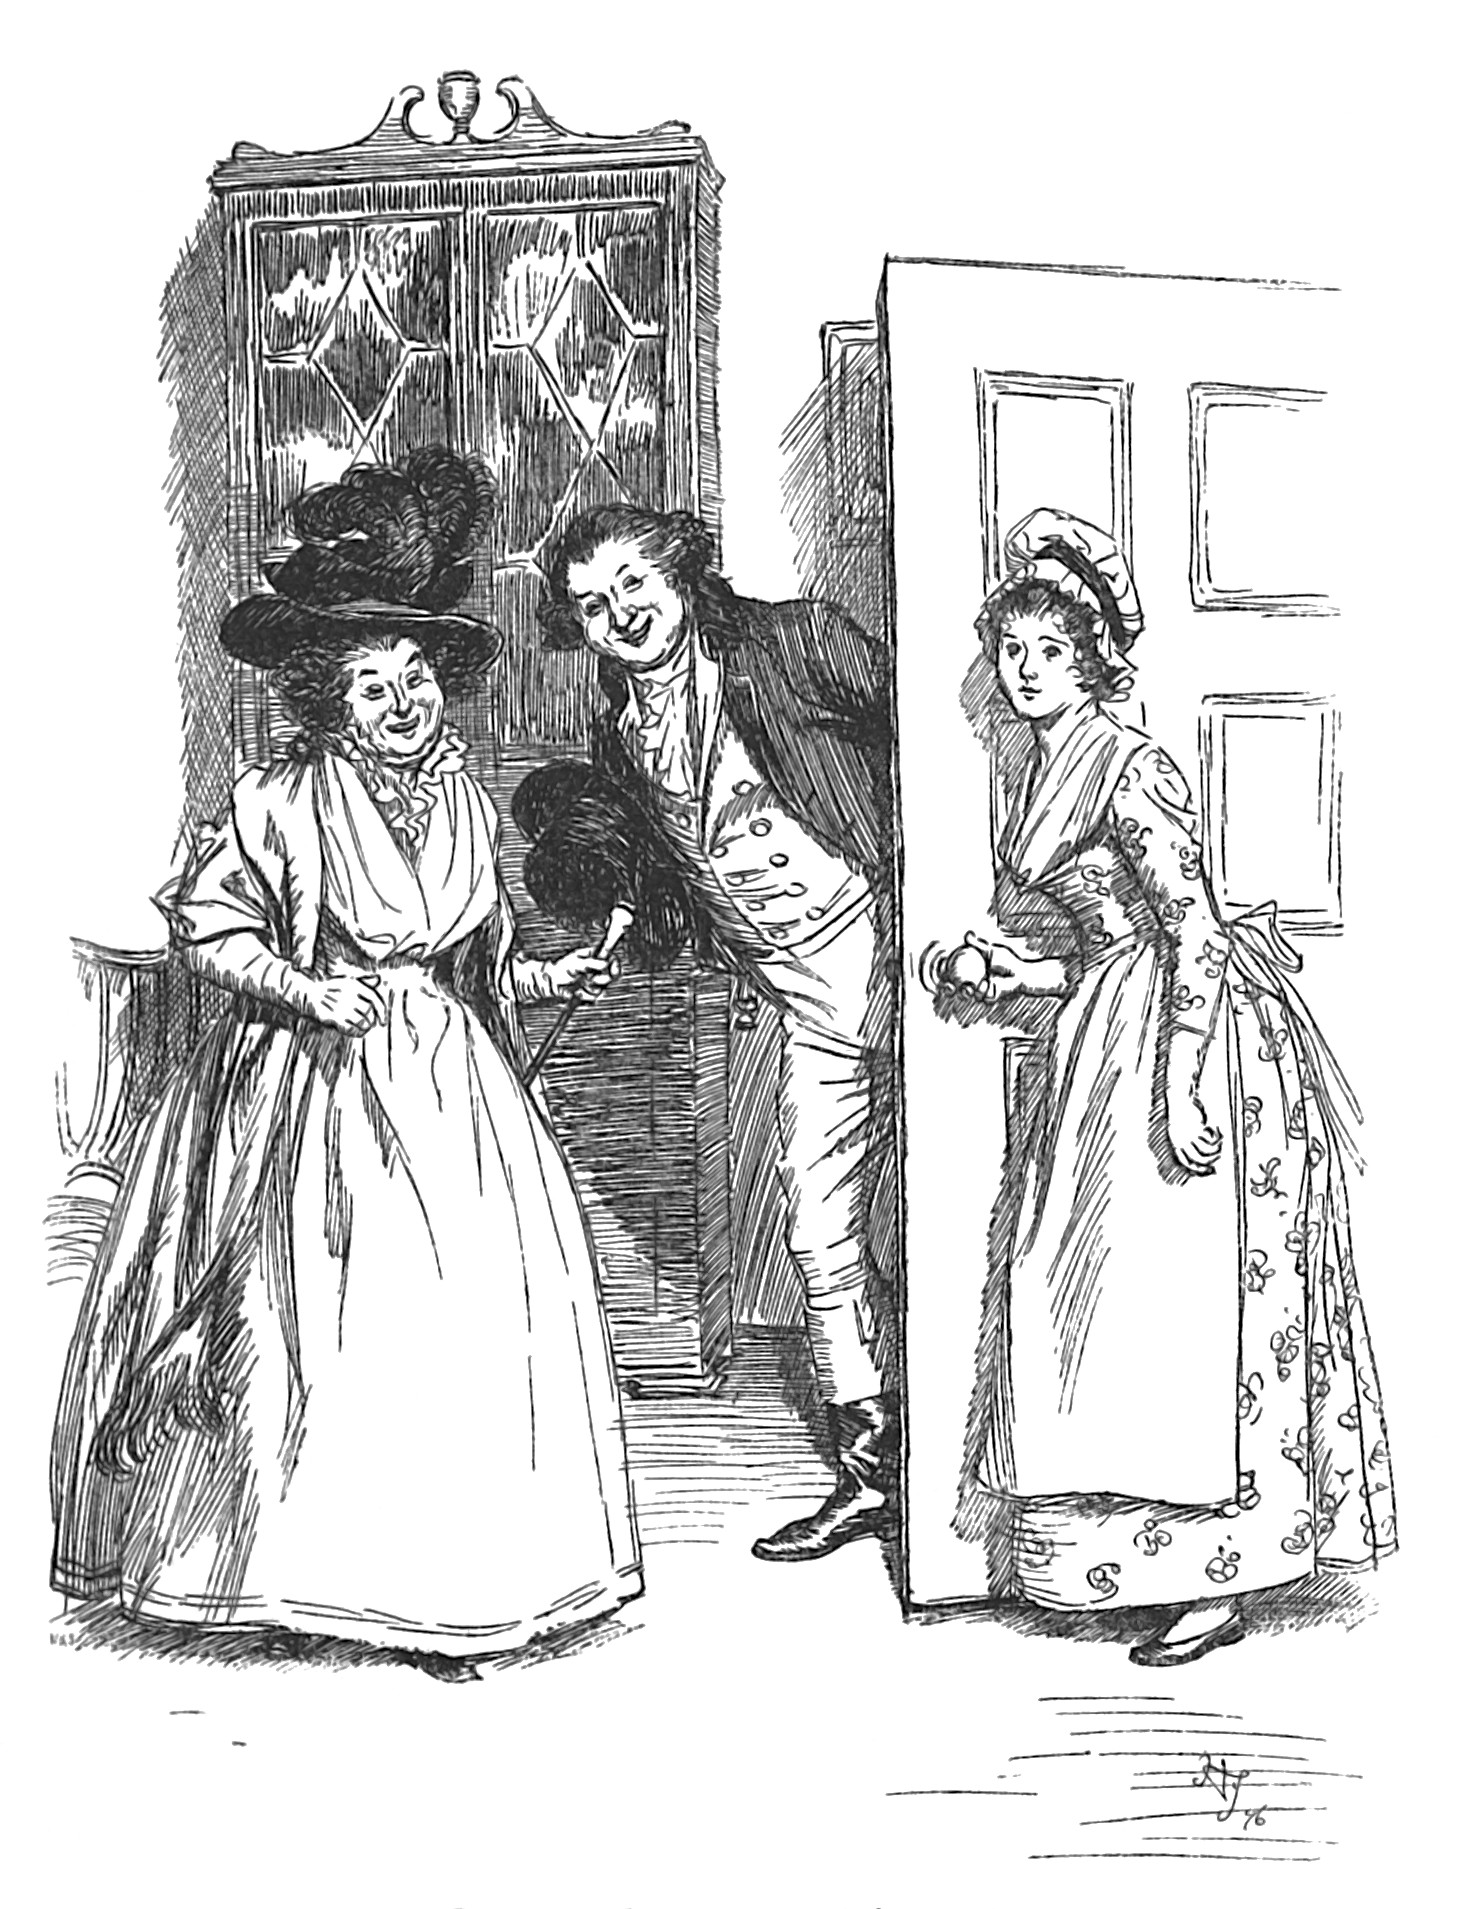
\includegraphics[width=\linewidth]{18guest}
\caption{Came to take a survey of the guest}
\end{figure}

Sir John never came to the Dashwoods without either inviting them to dine at the park the next day, or to drink tea with them that evening. On the present occasion, for the better entertainment of their visitor, towards whose amusement he felt himself bound to contribute, he wished to engage them for both.

»You \textit{must} drink tea with us to night,« said he, »for we shall be quite alone—and tomorrow you must absolutely dine with us, for we shall be a large party.«

Mrs Jennings enforced the necessity. »And who knows but \textit{you} may raise a dance,« said she. »And that will tempt you, Miss Marianne.«

»A dance!« cried Marianne. »Impossible! Who is to dance?«

»Who! why yourselves, and the Careys, and Whitakers to be sure.—What! you thought nobody could dance because a certain person that shall be nameless is gone!«

»I wish with all my soul,« cried Sir John, »that Willoughby were among us again.«

This, and Marianne’s blushing, gave new suspicions to Edward. »And who is Willoughby?« said he, in a low voice, to Miss Dashwood, by whom he was sitting.

She gave him a brief reply. Marianne’s countenance was more communicative. Edward saw enough to comprehend, not only the meaning of others, but such of Marianne’s expressions as had puzzled him before; and when their visitors left them, he went immediately round her, and said, in a whisper, »I have been guessing. Shall I tell you my guess?«

»What do you mean?«

»Shall I tell you?«

»Certainly.«

»Well then; I guess that Mr Willoughby hunts.«

Marianne was surprised and confused, yet she could not help smiling at the quiet archness of his manner, and after a moment’s silence, said,

»Oh, Edward! How can you?—But the time will come I hope...I am sure you will like him.«

»I do not doubt it,« replied he, rather astonished at her earnestness and warmth; for had he not imagined it to be a joke for the good of her acquaintance in general, founded only on a something or a nothing between Mr Willoughby and herself, he would not have ventured to mention it.
%!TeX root=../emmatop.tex
\chapter[Chapter \thechapter]{}
\lettrine[lraise=0.3]{E}{mma} and Harriet had been walking together one morning, and, in Emma's opinion, had been talking enough of Mr Elton for that day. She could not think that Harriet's solace or her own sins required more; and she was therefore industriously getting rid of the subject as they returned;—but it burst out again when she thought she had succeeded, and after speaking some time of what the poor must suffer in winter, and receiving no other answer than a very plaintive—<Mr Elton is so good to the poor!> she found something else must be done.

They were just approaching the house where lived Mrs and Miss Bates. She determined to call upon them and seek safety in numbers. There was always sufficient reason for such an attention; Mrs and Miss Bates loved to be called on, and she knew she was considered by the very few who presumed ever to see imperfection in her, as rather negligent in that respect, and as not contributing what she ought to the stock of their scanty comforts.

She had had many a hint from Mr Knightley and some from her own heart, as to her deficiency—but none were equal to counteract the persuasion of its being very disagreeable,—a waste of time—tiresome women—and all the horror of being in danger of falling in with the second-rate and third-rate of Highbury, who were calling on them for ever, and therefore she seldom went near them. But now she made the sudden resolution of not passing their door without going in—observing, as she proposed it to Harriet, that, as well as she could calculate, they were just now quite safe from any letter from Jane Fairfax.

The house belonged to people in business. Mrs and Miss Bates occupied the drawing-room floor; and there, in the very moderate-sized apartment, which was every thing to them, the visitors were most cordially and even gratefully welcomed; the quiet neat old lady, who with her knitting was seated in the warmest corner, wanting even to give up her place to Miss Woodhouse, and her more active, talking daughter, almost ready to overpower them with care and kindness, thanks for their visit, solicitude for their shoes, anxious inquiries after Mr Woodhouse's health, cheerful communications about her mother's, and sweet-cake from the beaufet—<Mrs Cole had just been there, just called in for ten minutes, and had been so good as to sit an hour with them, and she had taken a piece of cake and been so kind as to say she liked it very much; and, therefore, she hoped Miss Woodhouse and Miss Smith would do them the favour to eat a piece too.>

The mention of the Coles was sure to be followed by that of Mr Elton. There was intimacy between them, and Mr Cole had heard from Mr Elton since his going away. Emma knew what was coming; they must have the letter over again, and settle how long he had been gone, and how much he was engaged in company, and what a favourite he was wherever he went, and how full the Master of the Ceremonies' ball had been; and she went through it very well, with all the interest and all the commendation that could be requisite, and always putting forward to prevent Harriet's being obliged to say a word.

This she had been prepared for when she entered the house; but meant, having once talked him handsomely over, to be no farther incommoded by any troublesome topic, and to wander at large amongst all the Mistresses and Misses of Highbury, and their card-parties. She had not been prepared to have Jane Fairfax succeed Mr Elton; but he was actually hurried off by Miss Bates, she jumped away from him at last abruptly to the Coles, to usher in a letter from her niece.

<Oh! yes—Mr Elton, I understand—certainly as to dancing—Mrs Cole was telling me that dancing at the rooms at Bath was—Mrs Cole was so kind as to sit some time with us, talking of Jane; for as soon as she came in, she began inquiring after her, Jane is so very great a favourite there. Whenever she is with us, Mrs Cole does not know how to shew her kindness enough; and I must say that Jane deserves it as much as any body can. And so she began inquiring after her directly, saying, <I know you cannot have heard from Jane lately, because it is not her time for writing;> and when I immediately said, <But indeed we have, we had a letter this very morning,> I do not know that I ever saw any body more surprized. <Have you, upon your honour?> said she; <well, that is quite unexpected. Do let me hear what she says.>>

Emma's politeness was at hand directly, to say, with smiling interest—

<Have you heard from Miss Fairfax so lately? I am extremely happy. I hope she is well?>

\begin{figure}[tbph]
\centering

\includegraphics[width=\linewidth]{19hereitis}
\caption{<Oh! here it is.>}
\end{figure}

<Thank you. You are so kind!> replied the happily deceived aunt, while eagerly hunting for the letter.—<Oh! here it is. I was sure it could not be far off; but I had put my huswife upon it, you see, without being aware, and so it was quite hid, but I had it in my hand so very lately that I was almost sure it must be on the table. I was reading it to Mrs Cole, and since she went away, I was reading it again to my mother, for it is such a pleasure to her—a letter from Jane—that she can never hear it often enough; so I knew it could not be far off, and here it is, only just under my huswife—and since you are so kind as to wish to hear what she says;—but, first of all, I really must, in justice to Jane, apologise for her writing so short a letter—only two pages you see—hardly two—and in general she fills the whole paper and crosses half. My mother often wonders that I can make it out so well. She often says, when the letter is first opened, <Well, Hetty, now I think you will be put to it to make out all that checker-work>—don't you, ma'am?—And then I tell her, I am sure she would contrive to make it out herself, if she had nobody to do it for her—every word of it—I am sure she would pore over it till she had made out every word. And, indeed, though my mother's eyes are not so good as they were, she can see amazingly well still, thank God! with the help of spectacles. It is such a blessing! My mother's are really very good indeed. Jane often says, when she is here, <I am sure, grandmama, you must have had very strong eyes to see as you do—and so much fine work as you have done too!—I only wish my eyes may last me as well.>>

All this spoken extremely fast obliged Miss Bates to stop for breath; and Emma said something very civil about the excellence of Miss Fairfax's handwriting.

<You are extremely kind,> replied Miss Bates, highly gratified; <you who are such a judge, and write so beautifully yourself. I am sure there is nobody's praise that could give us so much pleasure as Miss Woodhouse's. My mother does not hear; she is a little deaf you know. Ma'am,> addressing her, <do you hear what Miss Woodhouse is so obliging to say about Jane's handwriting?>

And Emma had the advantage of hearing her own silly compliment repeated twice over before the good old lady could comprehend it. She was pondering, in the meanwhile, upon the possibility, without seeming very rude, of making her escape from Jane Fairfax's letter, and had almost resolved on hurrying away directly under some slight excuse, when Miss Bates turned to her again and seized her attention.

<My mother's deafness is very trifling you see—just nothing at all. By only raising my voice, and saying any thing two or three times over, she is sure to hear; but then she is used to my voice. But it is very remarkable that she should always hear Jane better than she does me. Jane speaks so distinct! However, she will not find her grandmama at all deafer than she was two years ago; which is saying a great deal at my mother's time of life—and it really is full two years, you know, since she was here. We never were so long without seeing her before, and as I was telling Mrs Cole, we shall hardly know how to make enough of her now.>

<Are you expecting Miss Fairfax here soon?>

<Oh yes; next week.>

<Indeed!—that must be a very great pleasure.>

<Thank you. You are very kind. Yes, next week. Every body is so surprized; and every body says the same obliging things. I am sure she will be as happy to see her friends at Highbury, as they can be to see her. Yes, Friday or Saturday; she cannot say which, because Colonel Campbell will be wanting the carriage himself one of those days. So very good of them to send her the whole way! But they always do, you know. Oh yes, Friday or Saturday next. That is what she writes about. That is the reason of her writing out of rule, as we call it; for, in the common course, we should not have heard from her before next Tuesday or Wednesday.>

<Yes, so I imagined. I was afraid there could be little chance of my hearing any thing of Miss Fairfax to-day.>

<So obliging of you! No, we should not have heard, if it had not been for this particular circumstance, of her being to come here so soon. My mother is so delighted!—for she is to be three months with us at least. Three months, she says so, positively, as I am going to have the pleasure of reading to you. The case is, you see, that the Campbells are going to Ireland. Mrs Dixon has persuaded her father and mother to come over and see her directly. They had not intended to go over till the summer, but she is so impatient to see them again—for till she married, last October, she was never away from them so much as a week, which must make it very strange to be in different kingdoms, I was going to say, but however different countries, and so she wrote a very urgent letter to her mother—or her father, I declare I do not know which it was, but we shall see presently in Jane's letter—wrote in Mr Dixon's name as well as her own, to press their coming over directly, and they would give them the meeting in Dublin, and take them back to their country seat, Baly-craig, a beautiful place, I fancy. Jane has heard a great deal of its beauty; from Mr Dixon, I mean—I do not know that she ever heard about it from any body else; but it was very natural, you know, that he should like to speak of his own place while he was paying his addresses—and as Jane used to be very often walking out with them—for Colonel and Mrs Campbell were very particular about their daughter's not walking out often with only Mr Dixon, for which I do not at all blame them; of course she heard every thing he might be telling Miss Campbell about his own home in Ireland; and I think she wrote us word that he had shewn them some drawings of the place, views that he had taken himself. He is a most amiable, charming young man, I believe. Jane was quite longing to go to Ireland, from his account of things.>

At this moment, an ingenious and animating suspicion entering Emma's brain with regard to Jane Fairfax, this charming Mr Dixon, and the not going to Ireland, she said, with the insidious design of farther discovery,

<You must feel it very fortunate that Miss Fairfax should be allowed to come to you at such a time. Considering the very particular friendship between her and Mrs Dixon, you could hardly have expected her to be excused from accompanying Colonel and Mrs Campbell.>

<Very true, very true, indeed. The very thing that we have always been rather afraid of; for we should not have liked to have her at such a distance from us, for months together—not able to come if any thing was to happen. But you see, every thing turns out for the best. They want her (Mr and Mrs Dixon) excessively to come over with Colonel and Mrs Campbell; quite depend upon it; nothing can be more kind or pressing than their joint invitation, Jane says, as you will hear presently; Mr Dixon does not seem in the least backward in any attention. He is a most charming young man. Ever since the service he rendered Jane at Weymouth, when they were out in that party on the water, and she, by the sudden whirling round of something or other among the sails, would have been dashed into the sea at once, and actually was all but gone, if he had not, with the greatest presence of mind, caught hold of her habit— (I can never think of it without trembling!)—But ever since we had the history of that day, I have been so fond of Mr Dixon!>

<But, in spite of all her friends' urgency, and her own wish of seeing Ireland, Miss Fairfax prefers devoting the time to you and Mrs Bates?>

<Yes—entirely her own doing, entirely her own choice; and Colonel and Mrs Campbell think she does quite right, just what they should recommend; and indeed they particularly wish her to try her native air, as she has not been quite so well as usual lately.>

<I am concerned to hear of it. I think they judge wisely. But Mrs Dixon must be very much disappointed. Mrs Dixon, I understand, has no remarkable degree of personal beauty; is not, by any means, to be compared with Miss Fairfax.>

<Oh! no. You are very obliging to say such things—but certainly not. There is no comparison between them. Miss Campbell always was absolutely plain—but extremely elegant and amiable.>

<Yes, that of course.>

<Jane caught a bad cold, poor thing! so long ago as the 7th of November, (as I am going to read to you,) and has never been well since. A long time, is not it, for a cold to hang upon her? She never mentioned it before, because she would not alarm us. Just like her! so considerate!—But however, she is so far from well, that her kind friends the Campbells think she had better come home, and try an air that always agrees with her; and they have no doubt that three or four months at Highbury will entirely cure her—and it is certainly a great deal better that she should come here, than go to Ireland, if she is unwell. Nobody could nurse her, as we should do.>

<It appears to me the most desirable arrangement in the world.>

<And so she is to come to us next Friday or Saturday, and the Campbells leave town in their way to Holyhead the Monday following—as you will find from Jane's letter. So sudden!—You may guess, dear Miss Woodhouse, what a flurry it has thrown me in! If it was not for the drawback of her illness—but I am afraid we must expect to see her grown thin, and looking very poorly. I must tell you what an unlucky thing happened to me, as to that. I always make a point of reading Jane's letters through to myself first, before I read them aloud to my mother, you know, for fear of there being any thing in them to distress her. Jane desired me to do it, so I always do: and so I began to-day with my usual caution; but no sooner did I come to the mention of her being unwell, than I burst out, quite frightened, with <Bless me! poor Jane is ill!>—which my mother, being on the watch, heard distinctly, and was sadly alarmed at. However, when I read on, I found it was not near so bad as I had fancied at first; and I make so light of it now to her, that she does not think much about it. But I cannot imagine how I could be so off my guard. If Jane does not get well soon, we will call in Mr Perry. The expense shall not be thought of; and though he is so liberal, and so fond of Jane that I dare say he would not mean to charge any thing for attendance, we could not suffer it to be so, you know. He has a wife and family to maintain, and is not to be giving away his time. Well, now I have just given you a hint of what Jane writes about, we will turn to her letter, and I am sure she tells her own story a great deal better than I can tell it for her.>

<I am afraid we must be running away,> said Emma, glancing at Harriet, and beginning to rise—<My father will be expecting us. I had no intention, I thought I had no power of staying more than five minutes, when I first entered the house. I merely called, because I would not pass the door without inquiring after Mrs Bates; but I have been so pleasantly detained! Now, however, we must wish you and Mrs Bates good morning.>

And not all that could be urged to detain her succeeded. She regained the street—happy in this, that though much had been forced on her against her will, though she had in fact heard the whole substance of Jane Fairfax's letter, she had been able to escape the letter itself.
%!TeX root=../pridetop.tex
\chapter[Chapter \thechapter]{}
\begin{figure}[t!]
\centering

\includegraphics[width=\linewidth]{20top}
\captionlistentry{Headpiece to Chapter \thechapter}
\end{figure}

\lettrine[lines=6,image=true]{initials/chap20m}{r}  Collins was not left long to the silent contemplation of his successful love; for Mrs Bennet, having dawdled about in the vestibule to watch for the end of the conference, no sooner saw Elizabeth open the door and with quick step pass her towards the staircase, than she entered the breakfast-room, and congratulated both him and herself in warm terms on the happy prospect of their nearer connection. Mr Collins received and returned these felicitations with equal pleasure, and then proceeded to relate the particulars of their interview, with the result of which he trusted he had every reason to be satisfied, since the refusal which his cousin had steadfastly given him would naturally flow from her bashful modesty and the genuine delicacy of her character.

This information, however, startled Mrs Bennet: she would have been glad to be equally satisfied that her daughter had meant to encourage him by protesting against his proposals, but she dared not believe it, and could not help saying so.

<But depend upon it, Mr Collins,> she added, <that Lizzy shall be brought to reason. I will speak to her about it myself directly. She is a very headstrong, foolish girl, and does not know her own interest; but I will \textit{make} her know it.>

<Pardon me for interrupting you, madam,> cried Mr Collins; <but if she is really headstrong and foolish, I know not whether she would altogether be a very desirable wife to a man in my situation, who naturally looks for happiness in the marriage state. If, therefore, she actually persists in rejecting my suit, perhaps it were better not to force her into accepting me, because, if liable to such defects of temper, she could not contribute much to my felicity.>

<Sir, you quite misunderstand me,> said Mrs Bennet, alarmed. <Lizzy is only headstrong in such matters as these. In everything else she is as good-natured a girl as ever lived. I will go directly to Mr Bennet, and we shall very soon settle it with her, I am sure.>

She would not give him time to reply, but hurrying instantly to her husband, called out, as she entered the library,—

<Oh, Mr Bennet, you are wanted immediately; we are all in an uproar. You must come and make Lizzy marry Mr Collins, for she vows she will not have him; and if you do not make haste he will change his mind and not have \textit{her}.>

Mr Bennet raised his eyes from his book as she entered, and fixed them on her face with a calm unconcern, which was not in the least altered by her communication.

<I have not the pleasure of understanding you,> said he, when she had finished her speech. <Of what are you talking?>

<Of Mr Collins and Lizzy. Lizzy declares she will not have Mr Collins, and Mr Collins begins to say that he will not have Lizzy.>

<And what am I to do on the occasion? It seems a hopeless business.>

<Speak to Lizzy about it yourself. Tell her that you insist upon her marrying him.>

<Let her be called down. She shall hear my opinion.>

Mrs Bennet rang the bell, and Miss Elizabeth was summoned to the library.

<Come here, child,> cried her father as she appeared. <I have sent for you on an affair of importance. I understand that Mr Collins has made you an offer of marriage. Is it true?>

Elizabeth replied that it was.

<Very well—and this offer of marriage you have refused?>

<I have, sir.>

<Very well. We now come to the point. Your mother insists upon your accepting it. Is it not so, Mrs Bennet?>

<Yes, or I will never see her again.>

<An unhappy alternative is before you, Elizabeth. From this day you must be a stranger to one of your parents. Your mother will never see you again if you do \textit{not} marry Mr Collins, and I will never see you again if you \textit{do}.>

Elizabeth could not but smile at such a conclusion of such a beginning; but Mrs Bennet, who had persuaded herself that her husband regarded the affair as she wished, was excessively disappointed.

<What do you mean, Mr Bennet, by talking in this way? You promised me to \textit{insist} upon her marrying him.>

<My dear,> replied her husband, <I have two small favours to request. First, that you will allow me the free use of my understanding on the present occasion; and, secondly, of my room. I shall be glad to have the library to myself as soon as may be.>

Not yet, however, in spite of her disappointment in her husband, did Mrs Bennet give up the point. She talked to Elizabeth again and again; coaxed and threatened her by turns. She endeavoured to secure Jane in her interest, but Jane, with all possible mildness, declined interfering; and Elizabeth, sometimes with real earnestness, and sometimes with playful gaiety, replied to her attacks. Though her manner varied, however, her determination never did.

Mr Collins, meanwhile, was meditating in solitude on what had passed. He thought too well of himself to comprehend on what motive his cousin could refuse him; and though his pride was hurt, he suffered in no other way. His regard for her was quite imaginary; and the possibility of her deserving her mother's reproach prevented his feeling any regret.

While the family were in this confusion, Charlotte Lucas came to spend the day with them. She was met in the vestibule by Lydia, who, flying to her, cried in a half whisper, <I am glad you are come, for there is such fun here! What do you think has happened this morning? Mr Collins has made an offer to Lizzy, and she will not have him.>

Charlotte had hardly time to answer before they were joined by Kitty, who came to tell the same news; and no sooner had they entered the breakfast-room, where Mrs Bennet was alone, than she likewise began on the subject, calling on Miss Lucas for her compassion, and entreating her to persuade her friend Lizzy to comply with the wishes of her family. <Pray do, my dear Miss Lucas,> she added, in a melancholy tone; <for nobody is on my side, nobody takes part with me; I am cruelly used, nobody feels for my poor nerves.>

\begin{figure}[tbh]
\centering

\includegraphics[width=.8\linewidth]{20breakfast}
\captionlistentry{They entered the breakfast room}
\end{figure}

Charlotte's reply was spared by the entrance of Jane and Elizabeth.

<Ay, there she comes,> continued Mrs Bennet, <looking as unconcerned as may be, and caring no more for us than if we were at York, provided she can have her own way. But I tell you what, Miss Lizzy, if you take it into your head to go on refusing every offer of marriage in this way, you will never get a husband at all—and I am sure I do not know who is to maintain you when your father is dead. \textit{I} shall not be able to keep you—and so I warn you. I have done with you from this very day. I told you in the library, you know, that I should never speak to you again, and you will find me as good as my word. I have no pleasure in talking to undutiful children. Not that I have much pleasure, indeed, in talking to anybody. People who suffer as I do from nervous complaints can have no great inclination for talking. Nobody can tell what I suffer! But it is always so. Those who do not complain are never pitied.>

Her daughters listened in silence to this effusion, sensible that any attempt to reason with or soothe her would only increase the irritation. She talked on, therefore, without interruption from any of them till they were joined by Mr Collins, who entered with an air more stately than usual, and on perceiving whom, she said to the girls,—

<Now, I do insist upon it, that you, all of you, hold your tongues, and let Mr Collins and me have a little conversation together.>

Elizabeth passed quietly out of the room, Jane and Kitty followed, but Lydia stood her ground, determined to hear all she could; and Charlotte, detained first by the civility of Mr Collins, whose inquiries after herself and all her family were very minute, and then by a little curiosity, satisfied herself with walking to the window and pretending not to hear. In a doleful voice Mrs Bennet thus began the projected conversation:—

<Oh, Mr Collins!>

<My dear madam,> replied he, <let us be for ever silent on this point. Far be it from me,> he presently continued, in a voice that marked his displeasure, <to resent the behaviour of your daughter. Resignation to inevitable evils is the duty of us all: the peculiar duty of a young man who has been so fortunate as I have been, in early preferment; and, I trust, I am resigned. Perhaps not the less so from feeling a doubt of my positive happiness had my fair cousin honoured me with her hand; for I have often observed, that resignation is never so perfect as when the blessing denied begins to lose somewhat of its value in our estimation. You will not, I hope, consider me as showing any disrespect to your family, my dear madam, by thus withdrawing my pretensions to your daughter's favour, without having paid yourself and Mr Bennet the compliment of requesting you to interpose your authority in my behalf. My conduct may, I fear, be objectionable in having accepted my dismission from your daughter's lips instead of your own; but we are all liable to error. I have certainly meant well through the whole affair. My object has been to secure an amiable companion for myself, with due consideration for the advantage of all your family; and if my \textit{manner} has been at all reprehensible, I here beg leave to apologize.>


\chapter[Chapter \thechapter]{} 

 \lettrine[lraise=0.3]{S}{ir} Thomas's return made a striking change in the ways of the family, independent of Lovers' Vows. Under his government, Mansfield was an altered place. Some members of their society sent away, and the spirits of many others saddened—it was all sameness and gloom compared with the past—a sombre family party rarely enlivened. There was little intercourse with the Parsonage. Sir~Thomas, drawing back from intimacies in general, was particularly disinclined, at this time, for any engagements but in one quarter. The Rushworths were the only addition to his own domestic circle which he could solicit.

Edmund did not wonder that such should be his father's feelings, nor could he regret anything but the exclusion of the Grants. <But they,> he observed to Fanny, <have a claim. They seem to belong to us; they seem to be part of ourselves. I could wish my father were more sensible of their very great attention to my mother and sisters while he was away. I am afraid they may feel themselves neglected. But the truth is, that my father hardly knows them. They had not been here a twelvemonth when he left England. If he knew them better, he would value their society as it deserves; for they are in fact exactly the sort of people he would like. We are sometimes a little in want of animation among ourselves: my sisters seem out of spirits, and Tom is certainly not at his ease. Dr~and Mrs~Grant would enliven us, and make our evenings pass away with more enjoyment even to my father.>

<Do you think so?> said Fanny: <in my opinion, my uncle would not like \textit{any}  addition. I think he values the very quietness you speak of, and that the repose of his own family circle is all he wants. And it does not appear to me that we are more serious than we used to be—I mean before my uncle went abroad. As well as I can recollect, it was always much the same. There was never much laughing in his presence; or, if there is any difference, it is not more, I think, than such an absence has a tendency to produce at first. There must be a sort of shyness; but I cannot recollect that our evenings formerly were ever merry, except when my uncle was in town. No young people's are, I suppose, when those they look up to are at home>.

<I believe you are right, Fanny,> was his reply, after a short consideration. <I believe our evenings are rather returned to what they were, than assuming a new character. The novelty was in their being lively. Yet, how strong the impression that only a few weeks will give! I have been feeling as if we had never lived so before.>

<I suppose I am graver than other people,> said Fanny. <The evenings do not appear long to me. I love to hear my uncle talk of the West Indies. I could listen to him for an hour together. It entertains \textit{me}  more than many other things have done; but then I am unlike other people, I dare say.>

<Why should you dare say \textit{that} ?> (smiling). <Do you want to be told that you are only unlike other people in being more wise and discreet? But when did you, or anybody, ever get a compliment from me, Fanny? Go to my father if you want to be complimented. He will satisfy you. Ask your uncle what he thinks, and you will hear compliments enough: and though they may be chiefly on your person, you must put up with it, and trust to his seeing as much beauty of mind in time.>

Such language was so new to Fanny that it quite embarrassed her.

<Your uncle thinks you very pretty, dear Fanny—and that is the long and the short of the matter. Anybody but myself would have made something more of it, and anybody but you would resent that you had not been thought very pretty before; but the truth is, that your uncle never did admire you till now—and now he does. Your complexion is so improved!—and you have gained so much countenance!—and your figure—nay, Fanny, do not turn away about it—it is but an uncle. If you cannot bear an uncle's admiration, what is to become of you? You must really begin to harden yourself to the idea of being worth looking at. You must try not to mind growing up into a pretty woman.>

<Oh! don't talk so, don't talk so,> cried Fanny, distressed by more feelings than he was aware of; but seeing that she was distressed, he had done with the subject, and only added more seriously—

<Your uncle is disposed to be pleased with you in every respect; and I only wish you would talk to him more. You are one of those who are too silent in the evening circle.>

<But I do talk to him more than I used. I am sure I do. Did not you hear me ask him about the slave-trade last night?>

<I did—and was in hopes the question would be followed up by others. It would have pleased your uncle to be inquired of farther.>

<And I longed to do it—but there was such a dead silence! And while my cousins were sitting by without speaking a word, or seeming at all interested in the subject, I did not like—I thought it would appear as if I wanted to set myself off at their expense, by shewing a curiosity and pleasure in his information which he must wish his own daughters to feel.>

<Miss~Crawford was very right in what she said of you the other day: that you seemed almost as fearful of notice and praise as other women were of neglect. We were talking of you at the Parsonage, and those were her words. She has great discernment. I know nobody who distinguishes characters better. For so young a woman it is remarkable! She certainly understands \textit{you}  better than you are understood by the greater part of those who have known you so long; and with regard to some others, I can perceive, from occasional lively hints, the unguarded expressions of the moment, that she could define \textit{many}  as accurately, did not delicacy forbid it. I wonder what she thinks of my father! She must admire him as a fine-looking man, with most gentlemanlike, dignified, consistent manners; but perhaps, having seen him so seldom, his reserve may be a little repulsive. Could they be much together, I feel sure of their liking each other. He would enjoy her liveliness and she has talents to value his powers. I wish they met more frequently! I hope she does not suppose there is any dislike on his side.>

<She must know herself too secure of the regard of all the rest of you,> said Fanny, with half a sigh, <to have any such apprehension. And Sir~Thomas's wishing just at first to be only with his family, is so very natural, that she can argue nothing from that. After a little while, I dare say, we shall be meeting again in the same sort of way, allowing for the difference of the time of year.>

<This is the first October that she has passed in the country since her infancy. I do not call Tunbridge or Cheltenham the country; and November is a still more serious month, and I can see that Mrs~Grant is very anxious for her not finding Mansfield dull as winter comes on.>

Fanny could have said a great deal, but it was safer to say nothing, and leave untouched all Miss~Crawford's resources—her accomplishments, her spirits, her importance, her friends, lest it should betray her into any observations seemingly unhandsome. Miss~Crawford's kind opinion of herself deserved at least a grateful forbearance, and she began to talk of something else.

<To-morrow, I think, my uncle dines at Sotherton, and you and Mr~Bertram too. We shall be quite a small party at home. I hope my uncle may continue to like Mr~Rushworth.>

<That is impossible, Fanny. He must like him less after to-morrow's visit, for we shall be five hours in his company. I should dread the stupidity of the day, if there were not a much greater evil to follow—the impression it must leave on Sir~Thomas. He cannot much longer deceive himself. I am sorry for them all, and would give something that Rushworth and Maria had never met.>

In this quarter, indeed, disappointment was impending over Sir~Thomas. Not all his good-will for Mr~Rushworth, not all Mr~Rushworth's deference for him, could prevent him from soon discerning some part of the truth—that Mr~Rushworth was an inferior young man, as ignorant in business as in books, with opinions in general unfixed, and without seeming much aware of it himself.

He had expected a very different son-in-law; and beginning to feel grave on Maria's account, tried to understand \textit{her}  feelings. Little observation there was necessary to tell him that indifference was the most favourable state they could be in. Her behaviour to Mr~Rushworth was careless and cold. She could not, did not like him. Sir~Thomas resolved to speak seriously to her. Advantageous as would be the alliance, and long standing and public as was the engagement, her happiness must not be sacrificed to it. Mr~Rushworth had, perhaps, been accepted on too short an acquaintance, and, on knowing him better, she was repenting.

With solemn kindness Sir~Thomas addressed her: told her his fears, inquired into her wishes, entreated her to be open and sincere, and assured her that every inconvenience should be braved, and the connexion entirely given up, if she felt herself unhappy in the prospect of it. He would act for her and release her. Maria had a moment's struggle as she listened, and only a moment's: when her father ceased, she was able to give her answer immediately, decidedly, and with no apparent agitation. She thanked him for his great attention, his paternal kindness, but he was quite mistaken in supposing she had the smallest desire of breaking through her engagement, or was sensible of any change of opinion or inclination since her forming it. She had the highest esteem for Mr~Rushworth's character and disposition, and could not have a doubt of her happiness with him.

Sir~Thomas was satisfied; too glad to be satisfied, perhaps, to urge the matter quite so far as his judgment might have dictated to others. It was an alliance which he could not have relinquished without pain; and thus he reasoned. Mr~Rushworth was young enough to improve. Mr~Rushworth must and would improve in good society; and if Maria could now speak so securely of her happiness with him, speaking certainly without the prejudice, the blindness of love, she ought to be believed. Her feelings, probably, were not acute; he had never supposed them to be so; but her comforts might not be less on that account; and if she could dispense with seeing her husband a leading, shining character, there would certainly be everything else in her favour. A well-disposed young woman, who did not marry for love, was in general but the more attached to her own family; and the nearness of Sotherton to Mansfield must naturally hold out the greatest temptation, and would, in all probability, be a continual supply of the most amiable and innocent enjoyments. Such and such-like were the reasonings of Sir~Thomas, happy to escape the embarrassing evils of a rupture, the wonder, the reflections, the reproach that must attend it; happy to secure a marriage which would bring him such an addition of respectability and influence, and very happy to think anything of his daughter's disposition that was most favourable for the purpose.

To her the conference closed as satisfactorily as to him. She was in a state of mind to be glad that she had secured her fate beyond recall: that she had pledged herself anew to Sotherton; that she was safe from the possibility of giving Crawford the triumph of governing her actions, and destroying her prospects; and retired in proud resolve, determined only to behave more cautiously to Mr~Rushworth in future, that her father might not be again suspecting her.

Had Sir~Thomas applied to his daughter within the first three or four days after Henry Crawford's leaving Mansfield, before her feelings were at all tranquillised, before she had given up every hope of him, or absolutely resolved on enduring his rival, her answer might have been different; but after another three or four days, when there was no return, no letter, no message, no symptom of a softened heart, no hope of advantage from separation, her mind became cool enough to seek all the comfort that pride and self revenge could give.

Henry Crawford had destroyed her happiness, but he should not know that he had done it; he should not destroy her credit, her appearance, her prosperity, too. He should not have to think of her as pining in the retirement of Mansfield for \textit{him}, rejecting Sotherton and London, independence and splendour, for \textit{his}  sake. Independence was more needful than ever; the want of it at Mansfield more sensibly felt. She was less and less able to endure the restraint which her father imposed. The liberty which his absence had given was now become absolutely necessary. She must escape from him and Mansfield as soon as possible, and find consolation in fortune and consequence, bustle and the world, for a wounded spirit. Her mind was quite determined, and varied not.

To such feelings delay, even the delay of much preparation, would have been an evil, and Mr~Rushworth could hardly be more impatient for the marriage than herself. In all the important preparations of the mind she was complete: being prepared for matrimony by an hatred of home, restraint, and tranquillity; by the misery of disappointed affection, and contempt of the man she was to marry. The rest might wait. The preparations of new carriages and furniture might wait for London and spring, when her own taste could have fairer play.

The principals being all agreed in this respect, it soon appeared that a very few weeks would be sufficient for such arrangements as must precede the wedding.

Mrs~Rushworth was quite ready to retire, and make way for the fortunate young woman whom her dear son had selected; and very early in November removed herself, her maid, her footman, and her chariot, with true dowager propriety, to Bath, there to parade over the wonders of Sotherton in her evening parties; enjoying them as thoroughly, perhaps, in the animation of a card-table, as she had ever done on the spot; and before the middle of the same month the ceremony had taken place which gave Sotherton another mistress.

It was a very proper wedding. The bride was elegantly dressed; the two bridesmaids were duly inferior; her father gave her away; her mother stood with salts in her hand, expecting to be agitated; her aunt tried to cry; and the service was impressively read by Dr~Grant. Nothing could be objected to when it came under the discussion of the neighbourhood, except that the carriage which conveyed the bride and bridegroom and Julia from the church-door to Sotherton was the same chaise which Mr~Rushworth had used for a twelvemonth before. In everything else the etiquette of the day might stand the strictest investigation.

It was done, and they were gone. Sir~Thomas felt as an anxious father must feel, and was indeed experiencing much of the agitation which his wife had been apprehensive of for herself, but had fortunately escaped. Mrs~Norris, most happy to assist in the duties of the day, by spending it at the Park to support her sister's spirits, and drinking the health of Mr~and Mrs~Rushworth in a supernumerary glass or two, was all joyous delight; for she had made the match; she had done everything; and no one would have supposed, from her confident triumph, that she had ever heard of conjugal infelicity in her life, or could have the smallest insight into the disposition of the niece who had been brought up under her eye.

The plan of the young couple was to proceed, after a few days, to Brighton, and take a house there for some weeks. Every public place was new to Maria, and Brighton is almost as gay in winter as in summer. When the novelty of amusement there was over, it would be time for the wider range of London.

Julia was to go with them to Brighton. Since rivalry between the sisters had ceased, they had been gradually recovering much of their former good understanding; and were at least sufficiently friends to make each of them exceedingly glad to be with the other at such a time. Some other companion than Mr~Rushworth was of the first consequence to his lady; and Julia was quite as eager for novelty and pleasure as Maria, though she might not have struggled through so much to obtain them, and could better bear a subordinate situation.

Their departure made another material change at Mansfield, a chasm which required some time to fill up. The family circle became greatly contracted; and though the Miss~Bertrams had latterly added little to its gaiety, they could not but be missed. Even their mother missed them; and how much more their tenderhearted cousin, who wandered about the house, and thought of them, and felt for them, with a degree of affectionate regret which they had never done much to deserve! 
%!TeX root=../emmatop.tex
\chapter[Chapter \thechapter]{}
\lettrine[lines=4,lraise=0.3]{H}{uman} nature is so well disposed towards those who are in interesting situations, that a young person, who either marries or dies, is sure of being kindly spoken of.

\zz
A week had not passed since Miss Hawkins's name was first mentioned in Highbury, before she was, by some means or other, discovered to have every recommendation of person and mind; to be handsome, elegant, highly accomplished, and perfectly amiable: and when Mr Elton himself arrived to triumph in his happy prospects, and circulate the fame of her merits, there was very little more for him to do, than to tell her Christian name, and say whose music she principally played.

Mr Elton returned, a very happy man. He had gone away rejected and mortified—disappointed in a very sanguine hope, after a series of what appeared to him strong encouragement; and not only losing the right lady, but finding himself debased to the level of a very wrong one. He had gone away deeply offended—he came back engaged to another—and to another as superior, of course, to the first, as under such circumstances what is gained always is to what is lost. He came back gay and self-satisfied, eager and busy, caring nothing for Miss Woodhouse, and defying Miss Smith.

The charming Augusta Hawkins, in addition to all the usual advantages of perfect beauty and merit, was in possession of an independent fortune, of so many thousands as would always be called ten; a point of some dignity, as well as some convenience: the story told well; he had not thrown himself away—he had gained a woman of 10,000 l. or thereabouts; and he had gained her with such delightful rapidity—the first hour of introduction had been so very soon followed by distinguishing notice; the history which he had to give Mrs Cole of the rise and progress of the affair was so glorious—the steps so quick, from the accidental rencontre, to the dinner at Mr Green's, and the party at Mrs Brown's—smiles and blushes rising in importance—with consciousness and agitation richly scattered—the lady had been so easily impressed—so sweetly disposed—had in short, to use a most intelligible phrase, been so very ready to have him, that vanity and prudence were equally contented.

He had caught both substance and shadow—both fortune and affection, and was just the happy man he ought to be; talking only of himself and his own concerns—expecting to be congratulated—ready to be laughed at—and, with cordial, fearless smiles, now addressing all the young ladies of the place, to whom, a few weeks ago, he would have been more cautiously gallant.

The wedding was no distant event, as the parties had only themselves to please, and nothing but the necessary preparations to wait for; and when he set out for Bath again, there was a general expectation, which a certain glance of Mrs Cole's did not seem to contradict, that when he next entered Highbury he would bring his bride.

During his present short stay, Emma had barely seen him; but just enough to feel that the first meeting was over, and to give her the impression of his not being improved by the mixture of pique and pretension, now spread over his air. She was, in fact, beginning very much to wonder that she had ever thought him pleasing at all; and his sight was so inseparably connected with some very disagreeable feelings, that, except in a moral light, as a penance, a lesson, a source of profitable humiliation to her own mind, she would have been thankful to be assured of never seeing him again. She wished him very well; but he gave her pain, and his welfare twenty miles off would administer most satisfaction.

The pain of his continued residence in Highbury, however, must certainly be lessened by his marriage. Many vain solicitudes would be prevented—many awkwardnesses smoothed by it. A Mrs Elton would be an excuse for any change of intercourse; former intimacy might sink without remark. It would be almost beginning their life of civility again.

Of the lady, individually, Emma thought very little. She was good enough for Mr Elton, no doubt; accomplished enough for Highbury—handsome enough—to look plain, probably, by Harriet's side. As to connexion, there Emma was perfectly easy; persuaded, that after all his own vaunted claims and disdain of Harriet, he had done nothing. On that article, truth seemed attainable. What she was, must be uncertain; but who she was, might be found out; and setting aside the 10,000 l., it did not appear that she was at all Harriet's superior. She brought no name, no blood, no alliance. Miss Hawkins was the youngest of the two daughters of a Bristol—merchant, of course, he must be called; but, as the whole of the profits of his mercantile life appeared so very moderate, it was not unfair to guess the dignity of his line of trade had been very moderate also. Part of every winter she had been used to spend in Bath; but Bristol was her home, the very heart of Bristol; for though the father and mother had died some years ago, an uncle remained—in the law line—nothing more distinctly honourable was hazarded of him, than that he was in the law line; and with him the daughter had lived. Emma guessed him to be the drudge of some attorney, and too stupid to rise. And all the grandeur of the connexion seemed dependent on the elder sister, who was very well married, to a gentleman in a great way, near Bristol, who kept two carriages! That was the wind-up of the history; that was the glory of Miss Hawkins.

Could she but have given Harriet her feelings about it all! She had talked her into love; but, alas! she was not so easily to be talked out of it. The charm of an object to occupy the many vacancies of Harriet's mind was not to be talked away. He might be superseded by another; he certainly would indeed; nothing could be clearer; even a Robert Martin would have been sufficient; but nothing else, she feared, would cure her. Harriet was one of those, who, having once begun, would be always in love. And now, poor girl! she was considerably worse from this reappearance of Mr Elton. She was always having a glimpse of him somewhere or other. Emma saw him only once; but two or three times every day Harriet was sure just to meet with him, or just to miss him, just to hear his voice, or see his shoulder, just to have something occur to preserve him in her fancy, in all the favouring warmth of surprize and conjecture. She was, moreover, perpetually hearing about him; for, excepting when at Hartfield, she was always among those who saw no fault in Mr Elton, and found nothing so interesting as the discussion of his concerns; and every report, therefore, every guess—all that had already occurred, all that might occur in the arrangement of his affairs, comprehending income, servants, and furniture, was continually in agitation around her. Her regard was receiving strength by invariable praise of him, and her regrets kept alive, and feelings irritated by ceaseless repetitions of Miss Hawkins's happiness, and continual observation of, how much he seemed attached!—his air as he walked by the house—the very sitting of his hat, being all in proof of how much he was in love!

Had it been allowable entertainment, had there been no pain to her friend, or reproach to herself, in the waverings of Harriet's mind, Emma would have been amused by its variations. Sometimes Mr Elton predominated, sometimes the Martins; and each was occasionally useful as a check to the other. Mr Elton's engagement had been the cure of the agitation of meeting Mr Martin. The unhappiness produced by the knowledge of that engagement had been a little put aside by Elizabeth Martin's calling at Mrs Goddard's a few days afterwards. Harriet had not been at home; but a note had been prepared and left for her, written in the very style to touch; a small mixture of reproach, with a great deal of kindness; and till Mr Elton himself appeared, she had been much occupied by it, continually pondering over what could be done in return, and wishing to do more than she dared to confess. But Mr Elton, in person, had driven away all such cares. While he staid, the Martins were forgotten; and on the very morning of his setting off for Bath again, Emma, to dissipate some of the distress it occasioned, judged it best for her to return Elizabeth Martin's visit.

How that visit was to be acknowledged—what would be necessary—and what might be safest, had been a point of some doubtful consideration. Absolute neglect of the mother and sisters, when invited to come, would be ingratitude. It must not be: and yet the danger of a renewal of the acquaintance—!

After much thinking, she could determine on nothing better, than Harriet's returning the visit; but in a way that, if they had understanding, should convince them that it was to be only a formal acquaintance. She meant to take her in the carriage, leave her at the Abbey Mill, while she drove a little farther, and call for her again so soon, as to allow no time for insidious applications or dangerous recurrences to the past, and give the most decided proof of what degree of intimacy was chosen for the future.

She could think of nothing better: and though there was something in it which her own heart could not approve—something of ingratitude, merely glossed over—it must be done, or what would become of Harriet?
%!TeX root=../emmatop.tex
\chapter[Chapter \thechapter]{}
\lettrine[lines=4,lraise=0.3]{S}{mall} heart had Harriet for visiting. Only half an hour before her friend called for her at Mrs Goddard's, her evil stars had led her to the very spot where, at that moment, a trunk, directed to The Rev. Philip Elton, White-Hart, Bath, was to be seen under the operation of being lifted into the butcher's cart, which was to convey it to where the coaches past; and every thing in this world, excepting that trunk and the direction, was consequently a blank.

She went, however; and when they reached the farm, and she was to be put down, at the end of the broad, neat gravel walk, which led between espalier apple-trees to the front door, the sight of every thing which had given her so much pleasure the autumn before, was beginning to revive a little local agitation; and when they parted, Emma observed her to be looking around with a sort of fearful curiosity, which determined her not to allow the visit to exceed the proposed quarter of an hour. She went on herself, to give that portion of time to an old servant who was married, and settled in Donwell.

The quarter of an hour brought her punctually to the white gate again; and Miss Smith receiving her summons, was with her without delay, and unattended by any alarming young man. She came solitarily down the gravel walk—a Miss Martin just appearing at the door, and parting with her seemingly with ceremonious civility.

\begin{figure}[tbph]
\centering

\includegraphics[width=.9\linewidth]{23room}
\caption{In that very room she had been measured}
\end{figure}

Harriet could not very soon give an intelligible account. She was feeling too much; but at last Emma collected from her enough to understand the sort of meeting, and the sort of pain it was creating. She had seen only Mrs Martin and the two girls. They had received her doubtingly, if not coolly; and nothing beyond the merest commonplace had been talked almost all the time—till just at last, when Mrs Martin's saying, all of a sudden, that she thought Miss Smith was grown, had brought on a more interesting subject, and a warmer manner. In that very room she had been measured last September, with her two friends. There were the pencilled marks and memorandums on the wainscot by the window. He had done it. They all seemed to remember the day, the hour, the party, the occasion—to feel the same consciousness, the same regrets—to be ready to return to the same good understanding; and they were just growing again like themselves, (Harriet, as Emma must suspect, as ready as the best of them to be cordial and happy,) when the carriage reappeared, and all was over. The style of the visit, and the shortness of it, were then felt to be decisive. Fourteen minutes to be given to those with whom she had thankfully passed six weeks not six months ago!—Emma could not but picture it all, and feel how justly they might resent, how naturally Harriet must suffer. It was a bad business. She would have given a great deal, or endured a great deal, to have had the Martins in a higher rank of life. They were so deserving, that a little higher should have been enough: but as it was, how could she have done otherwise?—Impossible!—She could not repent. They must be separated; but there was a great deal of pain in the process—so much to herself at this time, that she soon felt the necessity of a little consolation, and resolved on going home by way of Randalls to procure it. Her mind was quite sick of Mr Elton and the Martins. The refreshment of Randalls was absolutely necessary.

It was a good scheme; but on driving to the door they heard that neither »master nor mistress was at home;« they had both been out some time; the man believed they were gone to Hartfield.

»This is too bad,« cried Emma, as they turned away. »And now we shall just miss them; too provoking!—I do not know when I have been so disappointed.« And she leaned back in the corner, to indulge her murmurs, or to reason them away; probably a little of both—such being the commonest process of a not ill-disposed mind. Presently the carriage stopt; she looked up; it was stopt by Mr and Mrs Weston, who were standing to speak to her. There was instant pleasure in the sight of them, and still greater pleasure was conveyed in sound—for Mr Weston immediately accosted her with,

»How d'ye do?—how d'ye do?—We have been sitting with your father—glad to see him so well. Frank comes to-morrow—I had a letter this morning—we see him to-morrow by dinner-time to a certainty—he is at Oxford to-day, and he comes for a whole fortnight; I knew it would be so. If he had come at Christmas he could not have staid three days; I was always glad he did not come at Christmas; now we are going to have just the right weather for him, fine, dry, settled weather. We shall enjoy him completely; every thing has turned out exactly as we could wish.«

There was no resisting such news, no possibility of avoiding the influence of such a happy face as Mr Weston's, confirmed as it all was by the words and the countenance of his wife, fewer and quieter, but not less to the purpose. To know that she thought his coming certain was enough to make Emma consider it so, and sincerely did she rejoice in their joy. It was a most delightful reanimation of exhausted spirits. The worn-out past was sunk in the freshness of what was coming; and in the rapidity of half a moment's thought, she hoped Mr Elton would now be talked of no more.

Mr Weston gave her the history of the engagements at Enscombe, which allowed his son to answer for having an entire fortnight at his command, as well as the route and the method of his journey; and she listened, and smiled, and congratulated.

»I shall soon bring him over to Hartfield,« said he, at the conclusion.

Emma could imagine she saw a touch of the arm at this speech, from his wife.

»We had better move on, Mr Weston,« said she, »we are detaining the girls.«

»Well, well, I am ready;«—and turning again to Emma, »but you must not be expecting such a very fine young man; you have only had my account you know; I dare say he is really nothing extraordinary:«—though his own sparkling eyes at the moment were speaking a very different conviction.

Emma could look perfectly unconscious and innocent, and answer in a manner that appropriated nothing.

»Think of me to-morrow, my dear Emma, about four o'clock,« was Mrs Weston's parting injunction; spoken with some anxiety, and meant only for her.

»Four o'clock!—depend upon it he will be here by three,« was Mr Weston's quick amendment; and so ended a most satisfactory meeting. Emma's spirits were mounted quite up to happiness; every thing wore a different air; James and his horses seemed not half so sluggish as before. When she looked at the hedges, she thought the elder at least must soon be coming out; and when she turned round to Harriet, she saw something like a look of spring, a tender smile even there.

»Will Mr Frank Churchill pass through Bath as well as Oxford?«—was a question, however, which did not augur much.

But neither geography nor tranquillity could come all at once, and Emma was now in a humour to resolve that they should both come in time.

The morning of the interesting day arrived, and Mrs Weston's faithful pupil did not forget either at ten, or eleven, or twelve o'clock, that she was to think of her at four.

»My dear, dear anxious friend,«—said she, in mental soliloquy, while walking downstairs from her own room, »always overcareful for every body's comfort but your own; I see you now in all your little fidgets, going again and again into his room, to be sure that all is right.« The clock struck twelve as she passed through the hall. »'Tis twelve; I shall not forget to think of you four hours hence; and by this time to-morrow, perhaps, or a little later, I may be thinking of the possibility of their all calling here. I am sure they will bring him soon.«

She opened the parlour door, and saw two gentlemen sitting with her father—Mr Weston and his son. They had been arrived only a few minutes, and Mr Weston had scarcely finished his explanation of Frank's being a day before his time, and her father was yet in the midst of his very civil welcome and congratulations, when she appeared, to have her share of surprize, introduction, and pleasure.

The Frank Churchill so long talked of, so high in interest, was actually before her—he was presented to her, and she did not think too much had been said in his praise; he was a very good looking young man; height, air, address, all were unexceptionable, and his countenance had a great deal of the spirit and liveliness of his father's; he looked quick and sensible. She felt immediately that she should like him; and there was a well-bred ease of manner, and a readiness to talk, which convinced her that he came intending to be acquainted with her, and that acquainted they soon must be.

He had reached Randalls the evening before. She was pleased with the eagerness to arrive which had made him alter his plan, and travel earlier, later, and quicker, that he might gain half a day.

»I told you yesterday,« cried Mr Weston with exultation, »I told you all that he would be here before the time named. I remembered what I used to do myself. One cannot creep upon a journey; one cannot help getting on faster than one has planned; and the pleasure of coming in upon one's friends before the look-out begins, is worth a great deal more than any little exertion it needs.«

»It is a great pleasure where one can indulge in it,« said the young man, »though there are not many houses that I should presume on so far; but in coming home I felt I might do any thing.«

The word home made his father look on him with fresh complacency. Emma was directly sure that he knew how to make himself agreeable; the conviction was strengthened by what followed. He was very much pleased with Randalls, thought it a most admirably arranged house, would hardly allow it even to be very small, admired the situation, the walk to Highbury, Highbury itself, Hartfield still more, and professed himself to have always felt the sort of interest in the country which none but one's own country gives, and the greatest curiosity to visit it. That he should never have been able to indulge so amiable a feeling before, passed suspiciously through Emma's brain; but still, if it were a falsehood, it was a pleasant one, and pleasantly handled. His manner had no air of study or exaggeration. He did really look and speak as if in a state of no common enjoyment.

Their subjects in general were such as belong to an opening acquaintance. On his side were the inquiries,—»Was she a horsewoman?—Pleasant rides?—Pleasant walks?—Had they a large neighbourhood?—Highbury, perhaps, afforded society enough?—There were several very pretty houses in and about it.—Balls—had they balls?—Was it a musical society?«

But when satisfied on all these points, and their acquaintance proportionably advanced, he contrived to find an opportunity, while their two fathers were engaged with each other, of introducing his mother-in-law, and speaking of her with so much handsome praise, so much warm admiration, so much gratitude for the happiness she secured to his father, and her very kind reception of himself, as was an additional proof of his knowing how to please—and of his certainly thinking it worth while to try to please her. He did not advance a word of praise beyond what she knew to be thoroughly deserved by Mrs Weston; but, undoubtedly he could know very little of the matter. He understood what would be welcome; he could be sure of little else. »His father's marriage,« he said, »had been the wisest measure, every friend must rejoice in it; and the family from whom he had received such a blessing must be ever considered as having conferred the highest obligation on him.«

He got as near as he could to thanking her for Miss Taylor's merits, without seeming quite to forget that in the common course of things it was to be rather supposed that Miss Taylor had formed Miss Woodhouse's character, than Miss Woodhouse Miss Taylor's. And at last, as if resolved to qualify his opinion completely for travelling round to its object, he wound it all up with astonishment at the youth and beauty of her person.

»Elegant, agreeable manners, I was prepared for,« said he; »but I confess that, considering every thing, I had not expected more than a very tolerably well-looking woman of a certain age; I did not know that I was to find a pretty young woman in Mrs Weston.«

»You cannot see too much perfection in Mrs Weston for my feelings,« said Emma; »were you to guess her to be eighteen, I should listen with pleasure; but she would be ready to quarrel with you for using such words. Don't let her imagine that you have spoken of her as a pretty young woman.«

»I hope I should know better,« he replied; »no, depend upon it, (with a gallant bow,) that in addressing Mrs Weston I should understand whom I might praise without any danger of being thought extravagant in my terms.«

Emma wondered whether the same suspicion of what might be expected from their knowing each other, which had taken strong possession of her mind, had ever crossed his; and whether his compliments were to be considered as marks of acquiescence, or proofs of defiance. She must see more of him to understand his ways; at present she only felt they were agreeable.

She had no doubt of what Mr Weston was often thinking about. His quick eye she detected again and again glancing towards them with a happy expression; and even, when he might have determined not to look, she was confident that he was often listening.

Her own father's perfect exemption from any thought of the kind, the entire deficiency in him of all such sort of penetration or suspicion, was a most comfortable circumstance. Happily he was not farther from approving matrimony than from foreseeing it.—Though always objecting to every marriage that was arranged, he never suffered beforehand from the apprehension of any; it seemed as if he could not think so ill of any two persons' understanding as to suppose they meant to marry till it were proved against them. She blessed the favouring blindness. He could now, without the drawback of a single unpleasant surmise, without a glance forward at any possible treachery in his guest, give way to all his natural kind-hearted civility in solicitous inquiries after Mr Frank Churchill's accommodation on his journey, through the sad evils of sleeping two nights on the road, and express very genuine unmixed anxiety to know that he had certainly escaped catching cold—which, however, he could not allow him to feel quite assured of himself till after another night.

A reasonable visit paid, Mr Weston began to move.—»He must be going. He had business at the Crown about his hay, and a great many errands for Mrs Weston at Ford's, but he need not hurry any body else.« His son, too well bred to hear the hint, rose immediately also, saying,

»As you are going farther on business, sir, I will take the opportunity of paying a visit, which must be paid some day or other, and therefore may as well be paid now. I have the honour of being acquainted with a neighbour of yours, (turning to Emma,) a lady residing in or near Highbury; a family of the name of Fairfax. I shall have no difficulty, I suppose, in finding the house; though Fairfax, I believe, is not the proper name—I should rather say Barnes, or Bates. Do you know any family of that name?«

»To be sure we do,« cried his father; »Mrs Bates—we passed her house—I saw Miss Bates at the window. True, true, you are acquainted with Miss Fairfax; I remember you knew her at Weymouth, and a fine girl she is. Call upon her, by all means.«

»There is no necessity for my calling this morning,« said the young man; »another day would do as well; but there was that degree of acquaintance at Weymouth which\longdash«

»Oh! go to-day, go to-day. Do not defer it. What is right to be done cannot be done too soon. And, besides, I must give you a hint, Frank; any want of attention to her here should be carefully avoided. You saw her with the Campbells, when she was the equal of every body she mixed with, but here she is with a poor old grandmother, who has barely enough to live on. If you do not call early it will be a slight.«

The son looked convinced.

»I have heard her speak of the acquaintance,« said Emma; »she is a very elegant young woman.«

He agreed to it, but with so quiet a »Yes,« as inclined her almost to doubt his real concurrence; and yet there must be a very distinct sort of elegance for the fashionable world, if Jane Fairfax could be thought only ordinarily gifted with it.

»If you were never particularly struck by her manners before,« said she, »I think you will to-day. You will see her to advantage; see her and hear her—no, I am afraid you will not hear her at all, for she has an aunt who never holds her tongue.«

»You are acquainted with Miss Jane Fairfax, sir, are you?« said Mr Woodhouse, always the last to make his way in conversation; »then give me leave to assure you that you will find her a very agreeable young lady. She is staying here on a visit to her grandmama and aunt, very worthy people; I have known them all my life. They will be extremely glad to see you, I am sure; and one of my servants shall go with you to shew you the way.«

»My dear sir, upon no account in the world; my father can direct me.«

»But your father is not going so far; he is only going to the Crown, quite on the other side of the street, and there are a great many houses; you might be very much at a loss, and it is a very dirty walk, unless you keep on the footpath; but my coachman can tell you where you had best cross the street.«

Mr Frank Churchill still declined it, looking as serious as he could, and his father gave his hearty support by calling out, »My good friend, this is quite unnecessary; Frank knows a puddle of water when he sees it, and as to Mrs Bates's, he may get there from the Crown in a hop, step, and jump.«

They were permitted to go alone; and with a cordial nod from one, and a graceful bow from the other, the two gentlemen took leave. Emma remained very well pleased with this beginning of the acquaintance, and could now engage to think of them all at Randalls any hour of the day, with full confidence in their comfort.
%!TeX root=../sensetop.tex
\chapter[Chapter \thechapter]{}
\lettrine[lraise=0.3]{I}{n} a firm, though cautious tone, Elinor thus began.

\zz
<I should be undeserving of the confidence you have honoured me with, if I felt no desire for its continuance, or no farther curiosity on its subject. I will not apologize therefore for bringing it forward again.>

<Thank you,> cried Lucy warmly, <for breaking the ice; you have set my heart at ease by it; for I was somehow or other afraid I had offended you by what I told you that Monday.>

<Offended me! How could you suppose so? Believe me,> and Elinor spoke it with the truest sincerity, <nothing could be farther from my intention than to give you such an idea. Could you have a motive for the trust, that was not honourable and flattering to me?>

<And yet I do assure you,> replied Lucy, her little sharp eyes full of meaning, <there seemed to me to be a coldness and displeasure in your manner that made me quite uncomfortable. I felt sure that you was angry with me; and have been quarrelling with myself ever since, for having took such a liberty as to trouble you with my affairs. But I am very glad to find it was only my own fancy, and that you really do not blame me. If you knew what a consolation it was to me to relieve my heart speaking to you of what I am always thinking of every moment of my life, your compassion would make you overlook every thing else I am sure.>

<Indeed, I can easily believe that it was a very great relief to you, to acknowledge your situation to me, and be assured that you shall never have reason to repent it. Your case is a very unfortunate one; you seem to me to be surrounded with difficulties, and you will have need of all your mutual affection to support you under them. Mr Ferrars, I believe, is entirely dependent on his mother.>

<He has only two thousand pounds of his own; it would be madness to marry upon that, though for my own part, I could give up every prospect of more without a sigh. I have been always used to a very small income, and could struggle with any poverty for him; but I love him too well to be the selfish means of robbing him, perhaps, of all that his mother might give him if he married to please her. We must wait, it may be for many years. With almost every other man in the world, it would be an alarming prospect; but Edward's affection and constancy nothing can deprive me of I know.>

<That conviction must be every thing to you; and he is undoubtedly supported by the same trust in your's. If the strength of your reciprocal attachment had failed, as between many people, and under many circumstances it naturally would during a four years' engagement, your situation would have been pitiable, indeed.>

Lucy here looked up; but Elinor was careful in guarding her countenance from every expression that could give her words a suspicious tendency.

<Edward's love for me,> said Lucy, <has been pretty well put to the test, by our long, very long absence since we were first engaged, and it has stood the trial so well, that I should be unpardonable to doubt it now. I can safely say that he has never gave me one moment's alarm on that account from the first.>

Elinor hardly knew whether to smile or sigh at this assertion.

Lucy went on. <I am rather of a jealous temper too by nature, and from our different situations in life, from his being so much more in the world than me, and our continual separation, I was enough inclined for suspicion, to have found out the truth in an instant, if there had been the slightest alteration in his behaviour to me when we met, or any lowness of spirits that I could not account for, or if he had talked more of one lady than another, or seemed in any respect less happy at Longstaple than he used to be. I do not mean to say that I am particularly observant or quick-sighted in general, but in such a case I am sure I could not be deceived.>

<All this,> thought Elinor, <is very pretty; but it can impose upon neither of us.>

<But what,> said she after a short silence, <are your views? or have you none but that of waiting for Mrs Ferrars's death, which is a melancholy and shocking extremity?—Is her son determined to submit to this, and to all the tediousness of the many years of suspense in which it may involve you, rather than run the risk of her displeasure for a while by owning the truth?>

<If we could be certain that it would be only for a while! But Mrs Ferrars is a very headstrong proud woman, and in her first fit of anger upon hearing it, would very likely secure every thing to Robert, and the idea of that, for Edward's sake, frightens away all my inclination for hasty measures.>

<And for your own sake too, or you are carrying your disinterestedness beyond reason.>

Lucy looked at Elinor again, and was silent.

<Do you know Mr Robert Ferrars?> asked Elinor.

<Not at all—I never saw him; but I fancy he is very unlike his brother—silly and a great coxcomb.>

<A great coxcomb!> repeated Miss Steele, whose ear had caught those words by a sudden pause in Marianne's music. <Oh, they are talking of their favourite beaux, I dare say.>

<No sister,> cried Lucy, <you are mistaken there, our favourite beaux are \textit{not} great coxcombs.>

<I can answer for it that Miss Dashwood's is not,> said Mrs Jennings, laughing heartily; <for he is one of the modestest, prettiest behaved young men I ever saw; but as for Lucy, she is such a sly little creature, there is no finding out who \textit{she} likes.>

% \begin{figure}[tbph]
% \centering
% 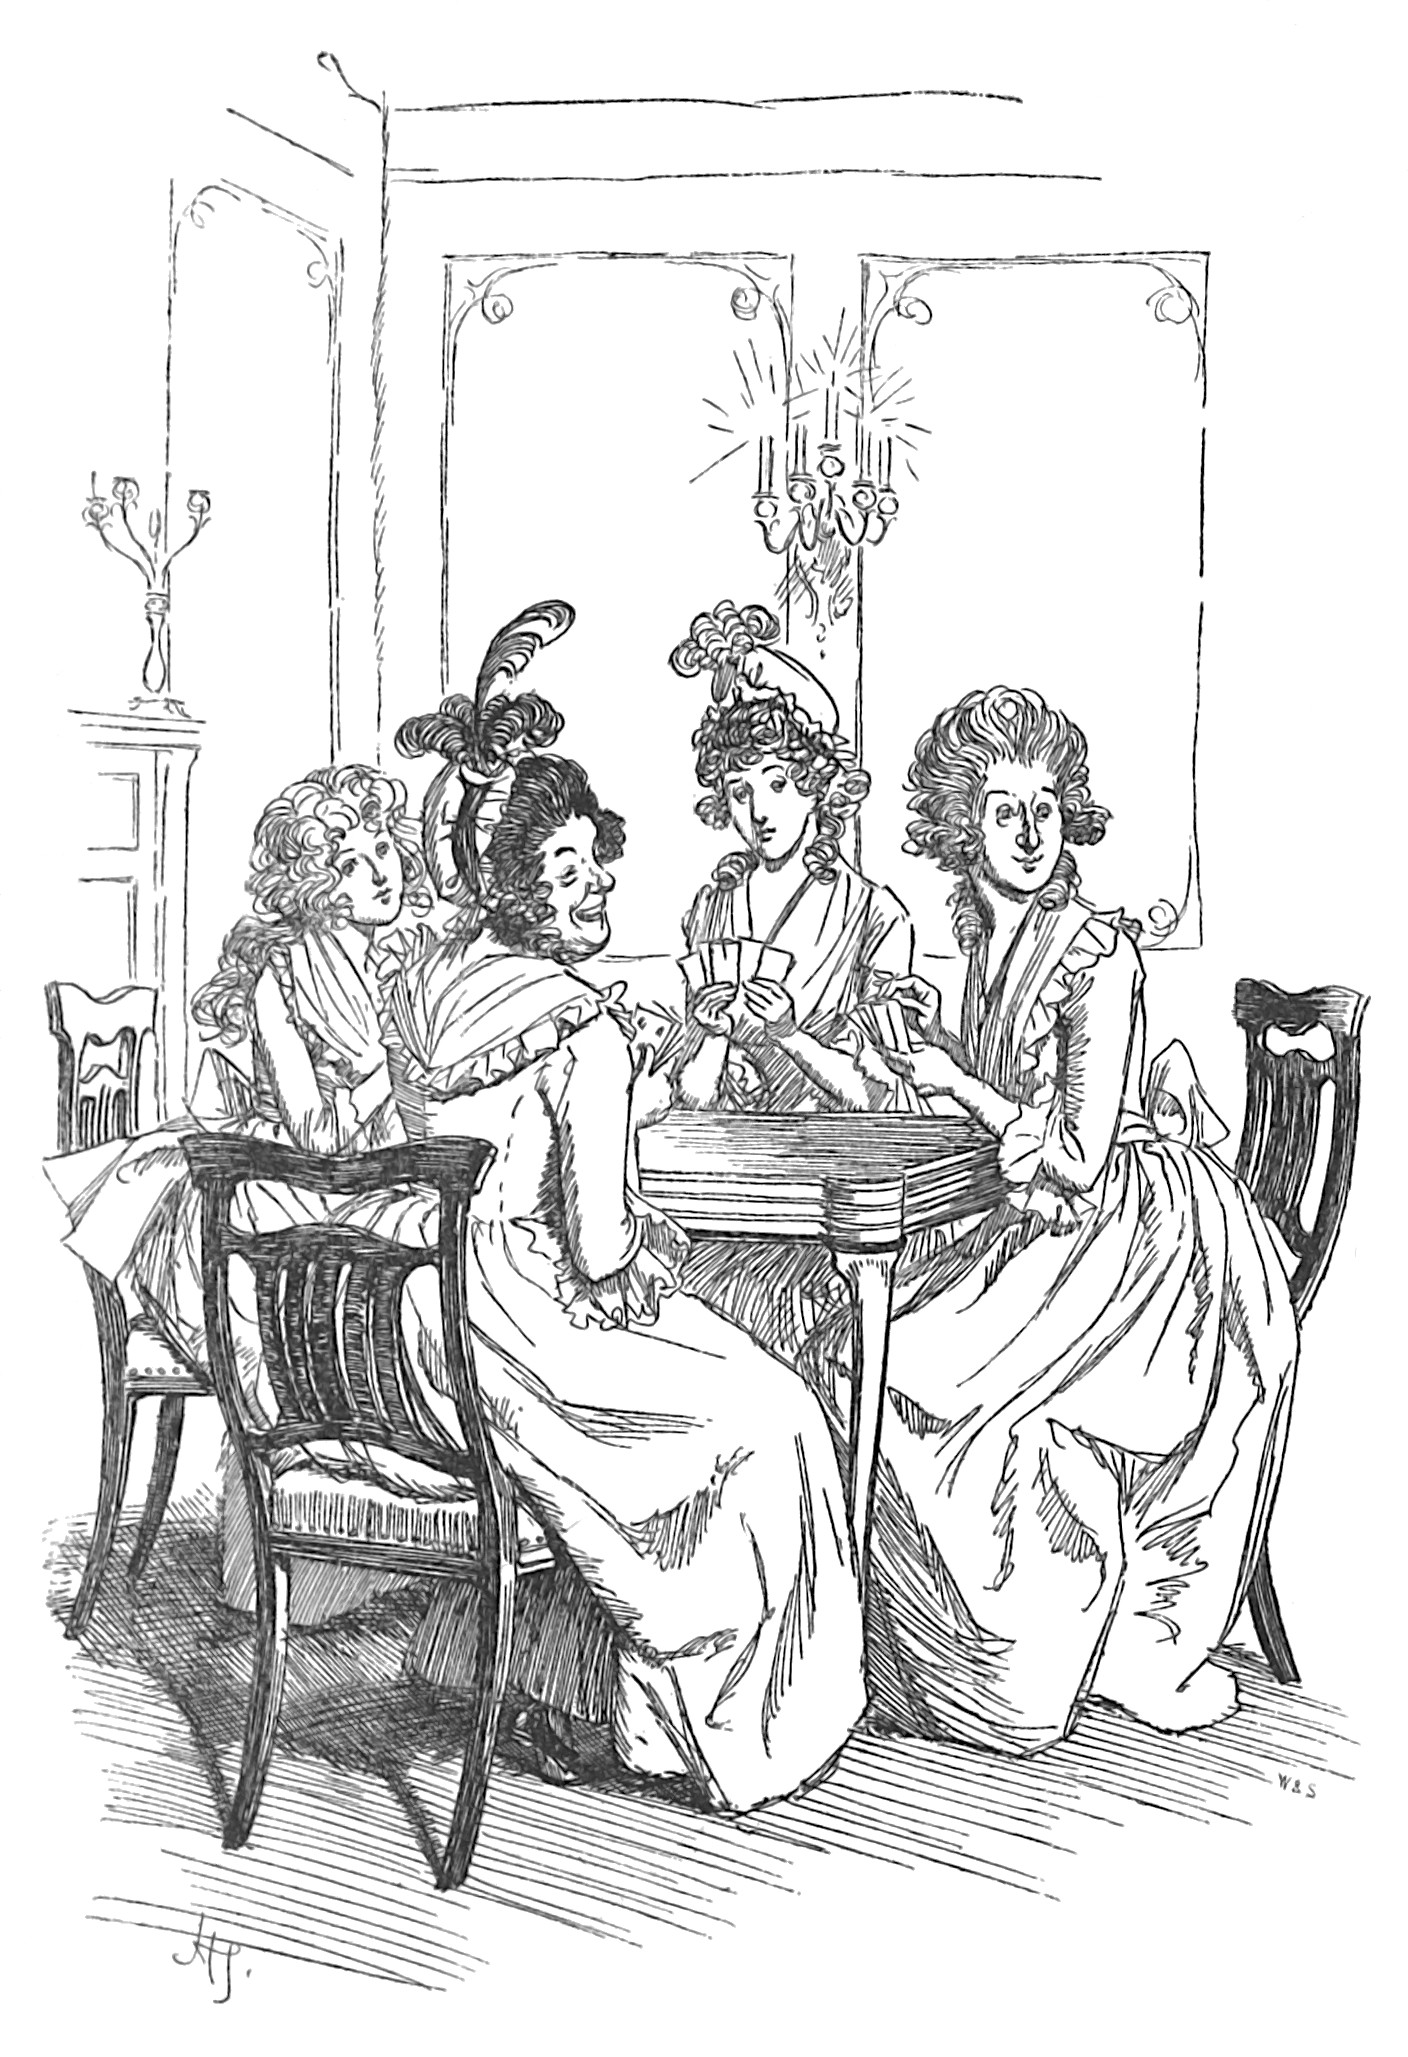
\includegraphics[width=\linewidth]{24answer}
% \caption{<I can answer for it,> said Mrs Jennings}
% \end{figure}

\begin{bwbigpic}
	[1.0]
	{24answer} 
	{<I can answer for it,> said Mrs Jennings} 
\end{bwbigpic}

<Oh,> cried Miss Steele, looking significantly round at them, <I dare say Lucy's beau is quite as modest and pretty behaved as Miss Dashwood's.>

Elinor blushed in spite of herself. Lucy bit her lip, and looked angrily at her sister. A mutual silence took place for some time. Lucy first put an end to it by saying in a lower tone, though Marianne was then giving them the powerful protection of a very magnificent concerto,—

<I will honestly tell you of one scheme which has lately come into my head, for bringing matters to bear; indeed I am bound to let you into the secret, for you are a party concerned. I dare say you have seen enough of Edward to know that he would prefer the church to every other profession; now my plan is that he should take orders as soon as he can, and then through your interest, which I am sure you would be kind enough to use out of friendship for him, and I hope out of some regard to me, your brother might be persuaded to give him Norland living; which I understand is a very good one, and the present incumbent not likely to live a great while. That would be enough for us to marry upon, and we might trust to time and chance for the rest.>

<I should always be happy,> replied Elinor, <to show any mark of my esteem and friendship for Mr Ferrars; but do you not perceive that my interest on such an occasion would be perfectly unnecessary? He is brother to Mrs John Dashwood—\textit{that} must be recommendation enough to her husband.>

<But Mrs John Dashwood would not much approve of Edward's going into orders.>

<Then I rather suspect that my interest would do very little.>

They were again silent for many minutes. At length Lucy exclaimed with a deep sigh,

<I believe it would be the wisest way to put an end to the business at once by dissolving the engagement. We seem so beset with difficulties on every side, that though it would make us miserable for a time, we should be happier perhaps in the end. But you will not give me your advice, Miss Dashwood?>

<No,> answered Elinor, with a smile, which concealed very agitated feelings, <on such a subject I certainly will not. You know very well that my opinion would have no weight with you, unless it were on the side of your wishes.>

<Indeed you wrong me,> replied Lucy, with great solemnity; <I know nobody of whose judgment I think so highly as I do of yours; and I do really believe, that if you was to say to me, <I advise you by all means to put an end to your engagement with Edward Ferrars, it will be more for the happiness of both of you,> I should resolve upon doing it immediately.>

Elinor blushed for the insincerity of Edward's future wife, and replied, <This compliment would effectually frighten me from giving any opinion on the subject had I formed one. It raises my influence much too high; the power of dividing two people so tenderly attached is too much for an indifferent person.>

<'Tis because you are an indifferent person,> said Lucy, with some pique, and laying a particular stress on those words, <that your judgment might justly have such weight with me. If you could be supposed to be biased in any respect by your own feelings, your opinion would not be worth having.>

Elinor thought it wisest to make no answer to this, lest they might provoke each other to an unsuitable increase of ease and unreserve; and was even partly determined never to mention the subject again. Another pause therefore of many minutes' duration, succeeded this speech, and Lucy was still the first to end it.

<Shall you be in town this winter, Miss Dashwood?> said she with all her accustomary complacency.

<Certainly not.>

<I am sorry for that,> returned the other, while her eyes brightened at the information, <it would have gave me such pleasure to meet you there! But I dare say you will go for all that. To be sure, your brother and sister will ask you to come to them.>

<It will not be in my power to accept their invitation if they do.>

<How unlucky that is! I had quite depended upon meeting you there. Anne and me are to go the latter end of January to some relations who have been wanting us to visit them these several years! But I only go for the sake of seeing Edward. He will be there in February, otherwise London would have no charms for me; I have not spirits for it.>

Elinor was soon called to the card-table by the conclusion of the first rubber, and the confidential discourse of the two ladies was therefore at an end, to which both of them submitted without any reluctance, for nothing had been said on either side to make them dislike each other less than they had done before; and Elinor sat down to the card table with the melancholy persuasion that Edward was not only without affection for the person who was to be his wife; but that he had not even the chance of being tolerably happy in marriage, which sincere affection on \textit{her} side would have given, for self-interest alone could induce a woman to keep a man to an engagement, of which she seemed so thoroughly aware that he was weary.

From this time the subject was never revived by Elinor, and when entered on by Lucy, who seldom missed an opportunity of introducing it, and was particularly careful to inform her confidante, of her happiness whenever she received a letter from Edward, it was treated by the former with calmness and caution, and dismissed as soon as civility would allow; for she felt such conversations to be an indulgence which Lucy did not deserve, and which were dangerous to herself.

The visit of the Miss Steeles at Barton Park was lengthened far beyond what the first invitation implied. Their favour increased; they could not be spared; Sir John would not hear of their going; and in spite of their numerous and long arranged engagements in Exeter, in spite of the absolute necessity of returning to fulfil them immediately, which was in full force at the end of every week, they were prevailed on to stay nearly two months at the park, and to assist in the due celebration of that festival which requires a more than ordinary share of private balls and large dinners to proclaim its importance.


\KOMAoptions{headings=openright}
%\KOMAoptions{fontsize=12.5pt}
%\vspace*{-2.5cm}


%\cleardoublepage
\RedeclareSectionCommand[afterskip=1cm,beforeskip=0cm]{chapter}
\KOMAoptions{headings=openleft}
\chapter*{}
\begin{figure}[t!]
\centering

\includegraphics[width=0.5\linewidth]{colophon}
\end{figure}

\centering

\vfill
\begin{minipage}{\textwidth}
\textit{Persuasion} was first published in December 1817 by John Murray in London (UK), after the death of Jane Austen (1775\textendash1817).
\end{minipage}
\vfill
gutenberg.org/ebooks/105
\vfill

\includegraphics[width=.4\textwidth]{flourish}
\vfill
\begin{minipage}{\textwidth}
Main text is set in <EB Garamond,> Georg Mayr-Duffner's free and open source implementation of Claude Garamond’s famous humanist typefaces from the mid-sixteenth century. Chapter headings are set in <Amarante>, by Karolina Lach. Dropcaps are set in <Floral Caps Nouveau>, by George Williams. Title page is set in <Bolton> and <Bolton Titling>, by Paul Lloyd.
\end{minipage}
\vfill
github.com/georgd/EB-Garamond\\
karolinalach.com\\
1001fonts.com/users/gww/\\
moorstation.org/typoasis/designers/lloyd/
\vfill

\includegraphics[width=.4\textwidth]{flourish}
\vfill
\begin{minipage}{\textwidth}
Title page decoration is by Dutch artist Willem Wenckebach (1860\textendash1937). The original is held by the Rijksmuseum in Amsterdam. Chapter decorations are from \textit{Twentieth Century Impressions of Hongkong, Shanghai, and other Treaty Ports of China} (ed. Arnold Wright), published in London in 1908.
\end{minipage}
\vfill

\includegraphics[width=.4\textwidth]{flourish}
\vfill
\begin{minipage}{\textwidth}
This typeset is dedicated to the public domain under a Creative Commons CC0 1.0 Universal deed: creativecommons.org/publicdomain/zero/1.0/
\end{minipage}
\vfill

\includegraphics[width=.4\textwidth]{flourish}
\vfill
Typeset in \LaTeX{}. Last revised \today.
\thispagestyle{empty}


\end{document}